\documentclass[aspectratio=169]{beamer}

\usepackage[utf8]{inputenc}

\usepackage{amsfonts}
\usepackage{amsmath}
\usepackage{amssymb}
\usepackage{color}
\usepackage{enumitem}
\usepackage{listings}
\usepackage{pifont}
\usepackage{tikz}
\usepackage{hyperref}
\usepackage{marvosym}

\usetikzlibrary {arrows,arrows.meta,positioning,shapes.misc}

\tikzset{stackframe/.style={
    % The shape:
    rectangle,
    % The size:
    minimum size=6mm,
    minimum width=50mm,
    % The border:
    thick,
    draw=black!80,
    % The filling:
    %top color=white, % a shading that is white at the top...
    %bottom color=red!50!black!20, % and something else at the bottom
    % Font
    font=\ttfamily
    },
    suspended/.style={
    rectangle,
    minimum size=6mm,
    minimum width=50mm,
    dotted,
    draw=black!80,
    font=\ttfamily,
    text=blue!50!black!50,
    },
    taskobj/.style={
    font=\ttfamily,
    minimum size=6mm,
    rectangle,rounded corners=3mm,
    top color=black!5, bottom color=black!25,
    },
}
\tikzstyle{every picture}+=[remember picture]

\newif\ifnotes
%  \notesfalse
  \notestrue

\ifnotes
\usepackage{pgfpages}
\setbeameroption{show notes}
\setbeameroption{show notes on second screen=right}
\fi

\usetheme{Rochester}
\usecolortheme{beaver}

\addtobeamertemplate{navigation symbols}{}{%
    \usebeamerfont{footline}%
    \usebeamercolor[fg]{footline}%
    \hspace{1em}%
    \insertframenumber/\inserttotalframenumber
}

\lstloadlanguages{C++}
    \lstset{%
        language={C++},
        basicstyle=\ttfamily,
        keywordstyle=\color{blue},
        showstringspaces=false,
        escapechar={§},
        escapeinside={(*@}{@*)}
    }

\lstdefinestyle{cpp20}{language={C++},
  morekeywords={noexcept,co_await,co_return,co_yield,requires,consteval,constinit,concept}
}

\newif\iftransitions
 \transitionstrue
% \transitionsfalse

\newcommand{\cpause}{\iftransitions \pause \fi}

\newcommand{\cuncover}[2]{\iftransitions \uncover<#1>{#2} \else #2 \fi}

\newcommand\monobox{}
\def\monobox[#1](#2:#3){\tikz[overlay]\filldraw[#1, opacity=0.3] ([shift={(0,-0.5ex)}]#2) rectangle ([shift={(0,2ex)}]#3);}

\newcommand\mixedbox{}
\def\mixedbox(#1:#2){\tikz[overlay]\filldraw[green, opacity=0.3]
  ([shift={(0,2ex)}]#2.center)
    -- ([shift={(0,-0.5ex)}]#1.center)
    -- ([shift={(0,-0.5ex)}]#2.center)
    -- cycle
    ;
  \tikz[overlay]\filldraw[blue, opacity=0.3]
  ([shift={(0,2ex)}]#1.center)
    -- ([shift={(0,-0.5ex)}]#1.center)
    -- ([shift={(0,2ex)}]#2.center)
    -- cycle
    ;}

\newcommand\danch{} 
\def\danch(#1){\tikz[baseline,inner sep=0]\node[anchor=base](#1){};}

\newif\iffast
% \fasttrue

\definecolor{co_return_object}{RGB}{179,179,255}
\definecolor{co_promise}{RGB}{255,179,179}
\definecolor{co_awaitable}{RGB}{179,255,179}
\definecolor{indigo}{RGB}{75,0,130}

\newlist{todolist}{itemize}{2}
\setlist[todolist]{label=$\square$}
\newcommand{\cmark}{\ding{51}}%
\newcommand{\xmark}{\ding{55}}%
\newcommand{\done}{\rlap{$\square$}{\raisebox{2pt}{\large\hspace{1pt}\cmark}}%
\hspace{-2.5pt}}
\newcommand{\wontfix}{\rlap{$\square$}{\large\hspace{1pt}\xmark}}


\title{Deciphering C++ Coroutines -}
\subtitle{Mastering Asynchronous Control Flow}
\author{Andreas Weis}
%\institute{...}

\date{ACCU 2025}
\titlegraphic{
\includegraphics[height=.15\textheight]{resources/accu_logo.png}}

\iffalse
Deciphering Coroutines - A Visual Approach

Coroutines are a powerful addition to C++20, allowing developers to drastically simplify code for certain kinds of problems and be adapted to a wide range of different use cases. But anyone trying to familiarize themselves with them will quickly notice that this flexibility comes at a price: In their current state, C++ coroutines are notoriously difficult to learn and their tight integration with the compiler gives them a feel quite unlike any other feature in the language.

The goal of this talk is to give a sustainable introduction on how to read and reason about coroutine code. We will learn how all the different elements of the mechanism fit together and to distinguish the parts of the code that follow the new rules of coroutines from those that still follow the well known conventional rules of C++. We will approach this through the construction of a coroutine cheat sheet, a collection of diagrams that serve as visual maps for navigating the complexities of the feature. Special care is taken to provide visual cues that are easily recognizable later on, to compensate for the fact that learners tend to forget the numerous details of the mechanism very fast if they don't use it in their everyday coding.

To account for the complexity of the topic, this talk focuses exclusively on providing a comprehensive introduction to the coroutine syntax, without discussing any advanced use cases. However, with the knowledge obtained from this talk, attendees will be able to easily follow more advanced presentations of coroutines later on without getting lost in the technical details of its peculiar syntax.


Outline:
- Essential Use Cases
 - Async Computation
 - Suspend/resume
- Understanding Coroutine Control Flow
- Coroutines from the Caller's Perspective
 - Coroutine Return Objects
- Coroutines Hello World Example
 - Coroutine Promise Type
 - Creation of the Coroutine Frame
 - Coroutine Handle
- Coroutine Suspension
 - Awaitables and Awaiters
- Lifetime of a Coroutine
- Drawing a Map of Coroutine Land
- Navigating Coroutine Land
 - Passing Data Into a Coroutine
 - Passing Data Out of a Coroutine
- Deciphering Advanced Coroutine Code


Deciphering C++ Coroutines - Mastering Asynchronous Control Flow

One of the most powerful applications of coroutines is in the context of asynchronous operations, where their use allows for significant simplifactions of application code. Unfortunately, building an asynchronous library interface to enable such benefits for applications is not exactly straightforward in C++.

In this talk we will explore the essentials of managing asynchronous control flow with coroutines. We will discover how to reconstruct the call stack of nested asynchronous calls and thus bridge a significant gap between C++'s stackless coroutines and the stackful coroutines from other languages. We will learn how to build a mechanism similar to the async/await from languages like Python or Javascript for our own libraries. And we will explore how we can perform arbitrary manipulations of the call stack in such an environment to unleash the full power of C++'s coroutine mechanism.

At the end of this talk we will have a proper understanding of how the Task<> type found in many coroutine libraries works and how it can be used to manage asynchronous operations. This will serve as an important building block for understanding more advanced mechanisms, like the sender/receiver mechanism proposed for C++26.

This talk assumes basic familiarity with the components of the C++ coroutines language feature: promises, awaitables, coroutine handles, and passing data in and out of coroutines.

This is the second part in an ongoing series of talks about C++20 coroutines.

Outline:
This talk is aimed at people who understand the basics of the coroutine language mechanism, but not how to use them in an asynchronous context. The goal is to teach a programmer that knows how a generator<> works how to write their own task<>.

* Very short recap of C++20 coroutines
* Control flow in synchronous and asynchronous programs
* The problem of the lost program stack in asynchronous code
* The dual role of the task<> return type
* Preserving the call stack in the task<> type
* Building async/await in C++
* Traversing the call stack to resume nested function calls
* Resuming asynchronous functions from an executor
* Lazy vs. eager execution of tasks
* Non-obvious resumption patterns and manipulations of the call stack
\fi

\begin{document}
{ % all template changes are local to this group.
    \setbeamertemplate{navigation symbols}{}
    \begin{frame}<article:0>[plain]
        \begin{tikzpicture}[remember picture,overlay]
            \node[at=(current page.center)] {
                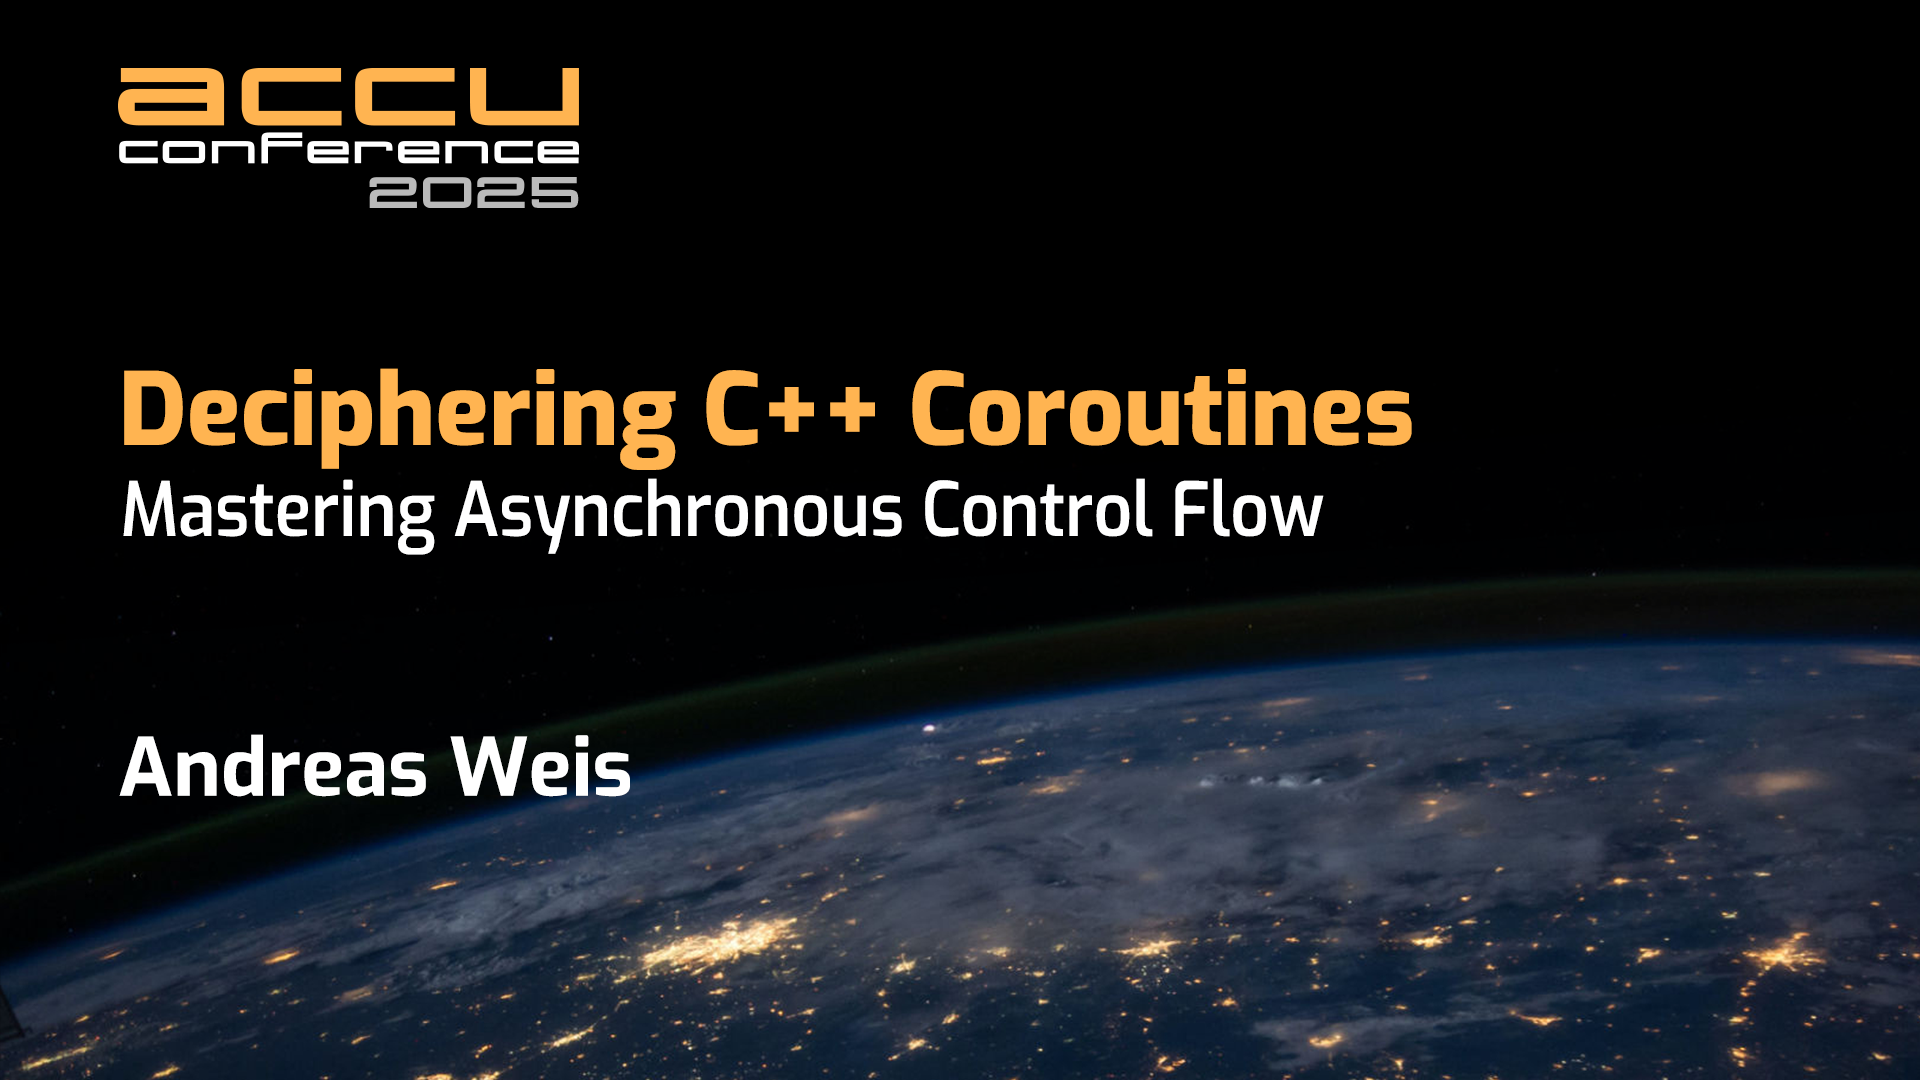
\includegraphics[keepaspectratio,
                                 width=\paperwidth,
                                 height=\paperheight]{corogfx2/accu_title_card.png}
            };
        \end{tikzpicture}
     \end{frame}
}

\frame{\titlepage}

\iftrue %crop
\fi

% \iffalse % !!!!!!!!!!!!!!

\begin{frame}[fragile]
  \frametitle{About me - Andreas Weis (he/him)}

  \begin{itemize}
    \setlength\itemsep{1.5em}

    \item \href{https://stackoverflow.com/users/577603/comicsansms}{
\includegraphics[height=.05\textheight]{resources/so-icon.png}} \href{https://github.com/ComicSansMS}{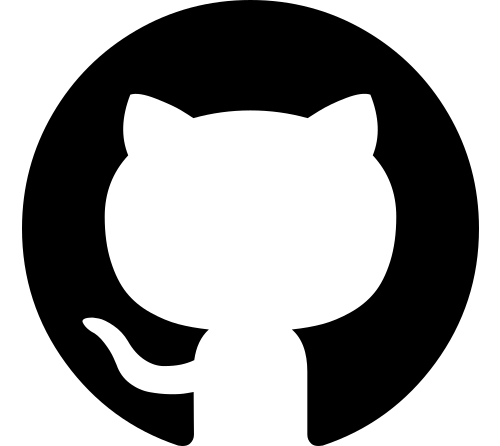
\includegraphics[height=.05\textheight]{resources/github-icon.png}} \includegraphics[height=.05\textheight]{resources/discord-icon.png} ComicSansMS

    %\item \href{https://twitter.com/DerGhulbus/}{
\includegraphics[height=.05\textheight]{resources/twitter-icon.png} @DerGhulbus}

    \item \href{mailto:cpp@andreas-weis.net}{
\includegraphics[height=.06\textheight]{resources/email-icon.png} cpp@andreas-weis.net}

    \item \href{https://www.meetup.com/MUCplusplus/}{
\includegraphics[height=.05\textheight]{resources/meetup-icon.png}} Co-organizer of the \href{https://www.meetup.com/MUCplusplus/}{Munich C++ User Group}
  \end{itemize}
\end{frame}

\begin{frame}
  \frametitle{The story so far...}

  \begin{center}
    \href{https://www.youtube.com/watch?v=J7fYddslH0Q}{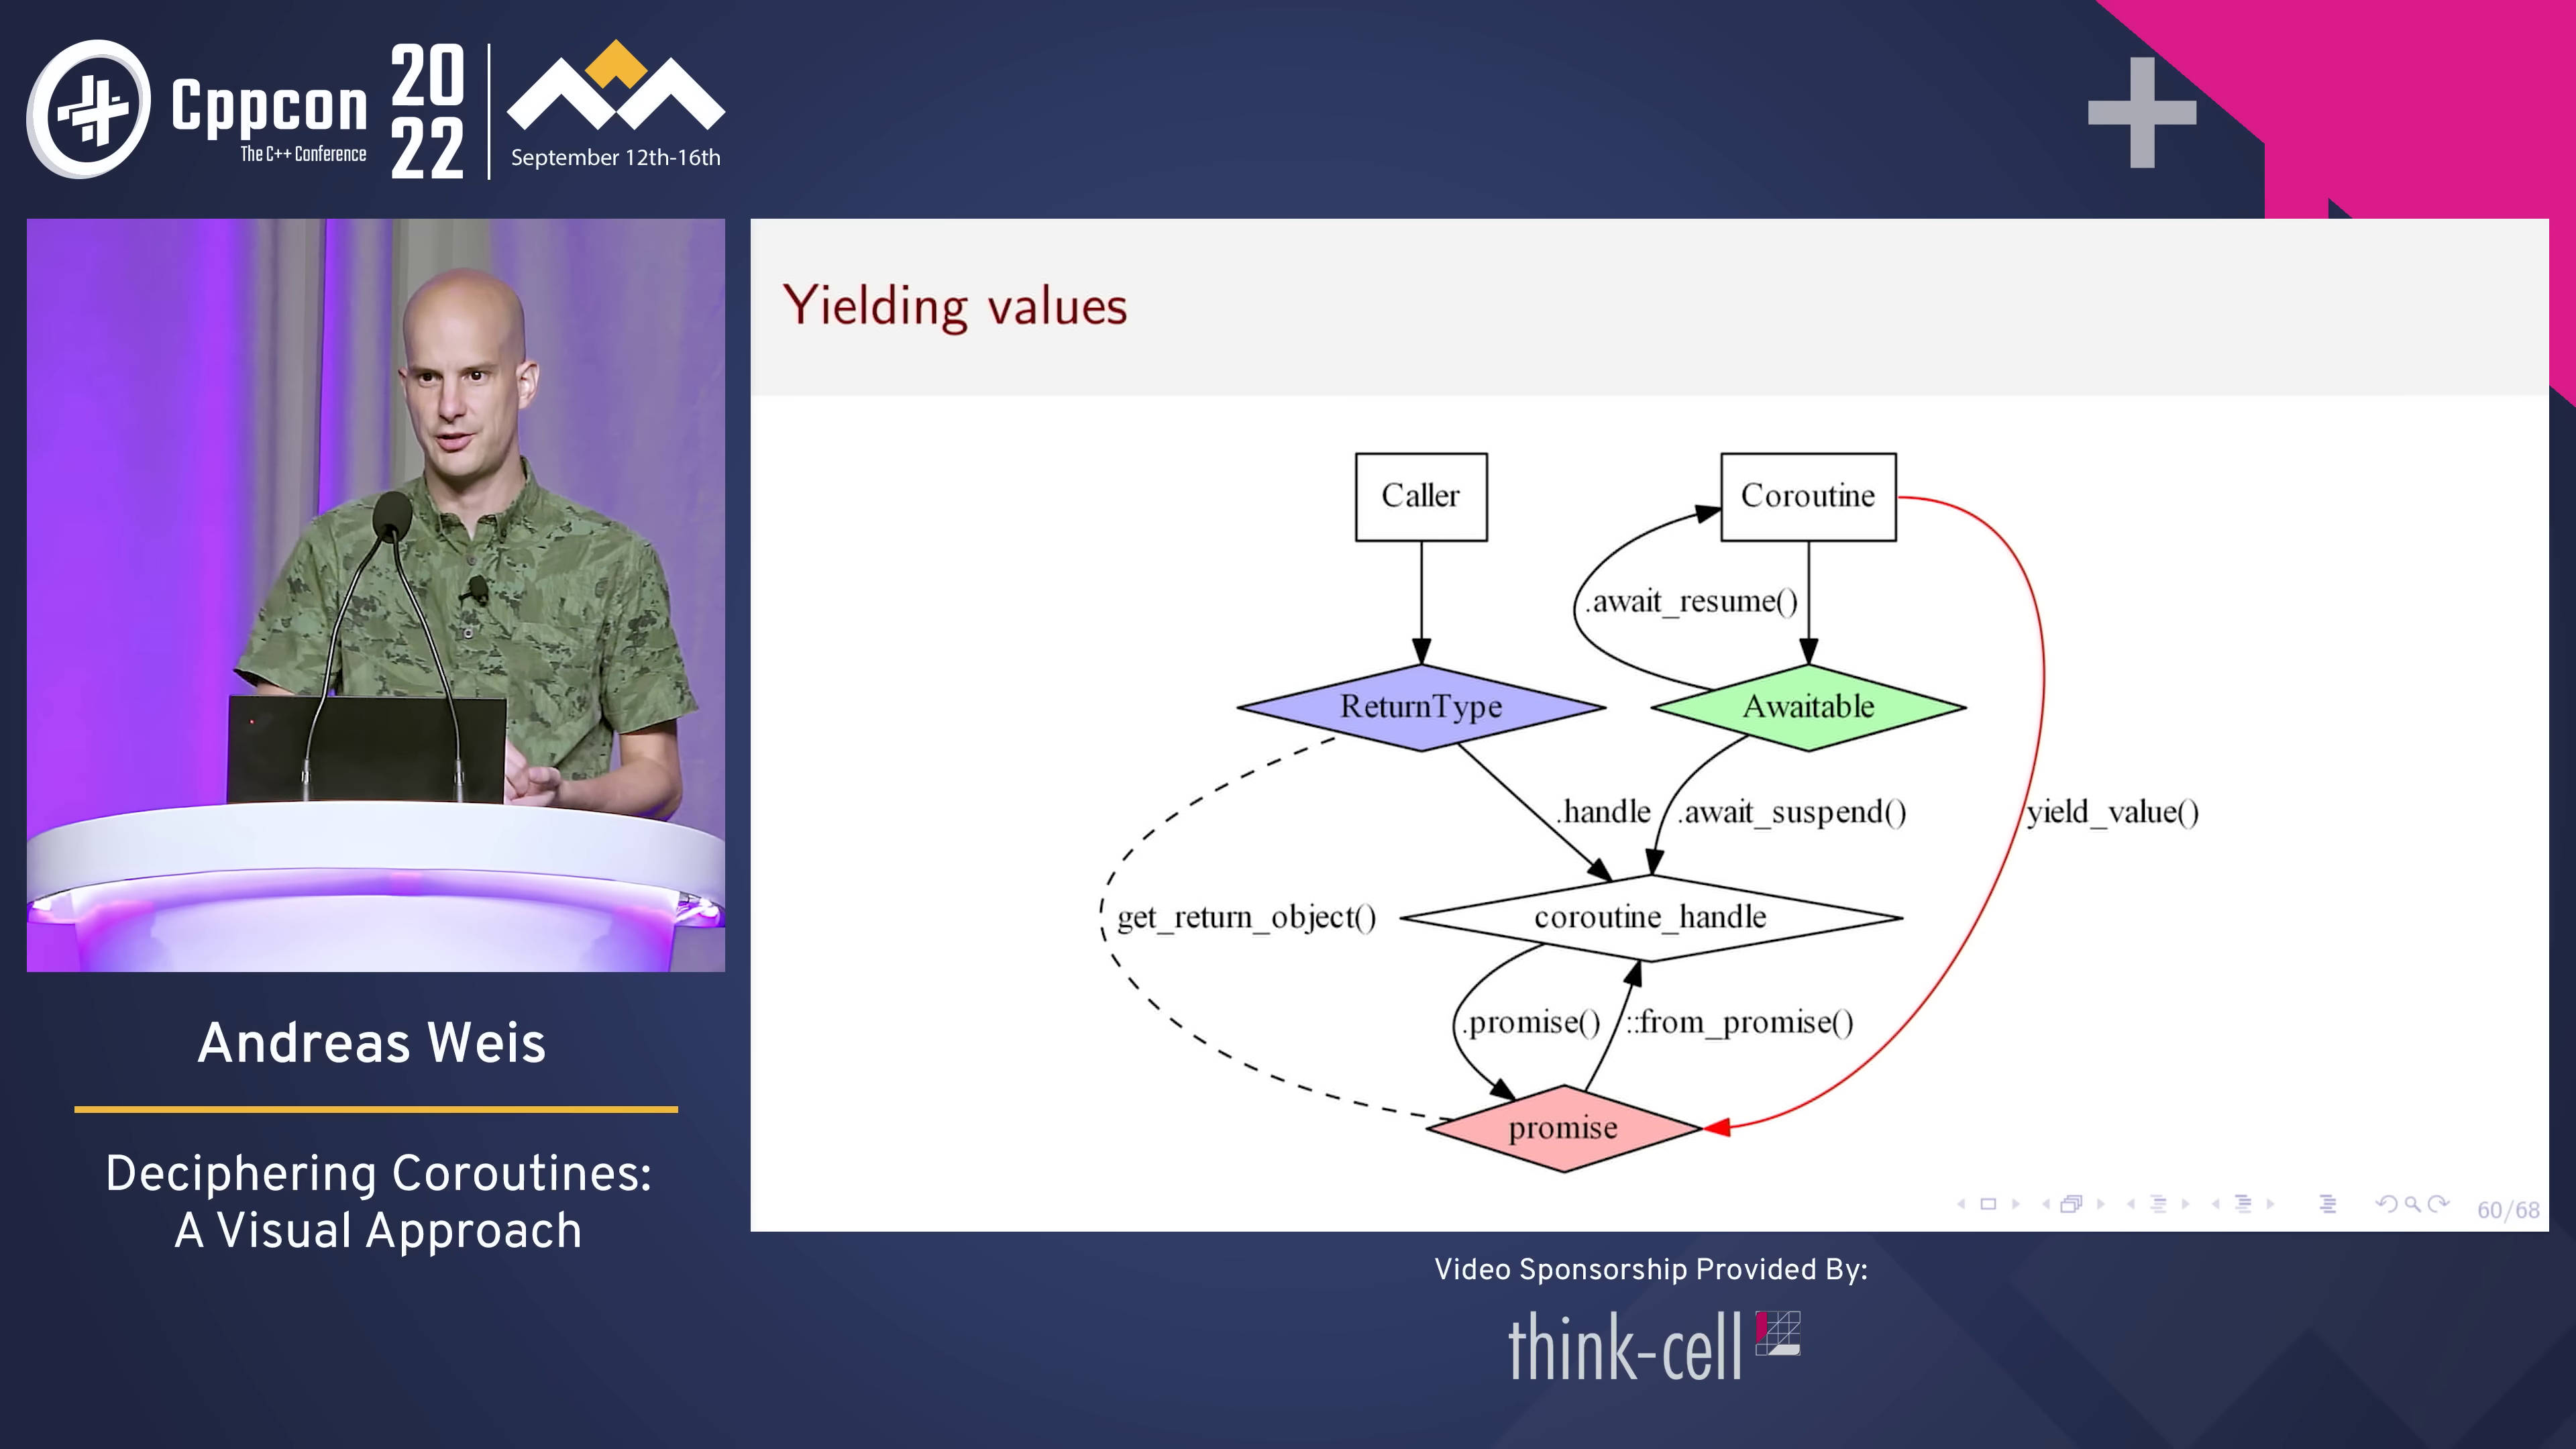
\includegraphics[height=.80\textheight]{corogfx2/talk_deciphering_part1.jpg}}
  \end{center}

  \note{
  \begin{itemize}
  \item This is part 2 of a series of talks on coroutines. \\ You can find part 1 from two years ago on Youtube. \\ This talk assumes that you are familiar with the contents of part 1, that is, you should know the basic mechanisms of the coroutine language mechanics. \\ We will do a quick recap of part 1 now, but it will be very brief, so hang on tight.
  \end{itemize}
  }
\end{frame}

\begin{frame}
  \frametitle{Where we left off...}

  \begin{center}
  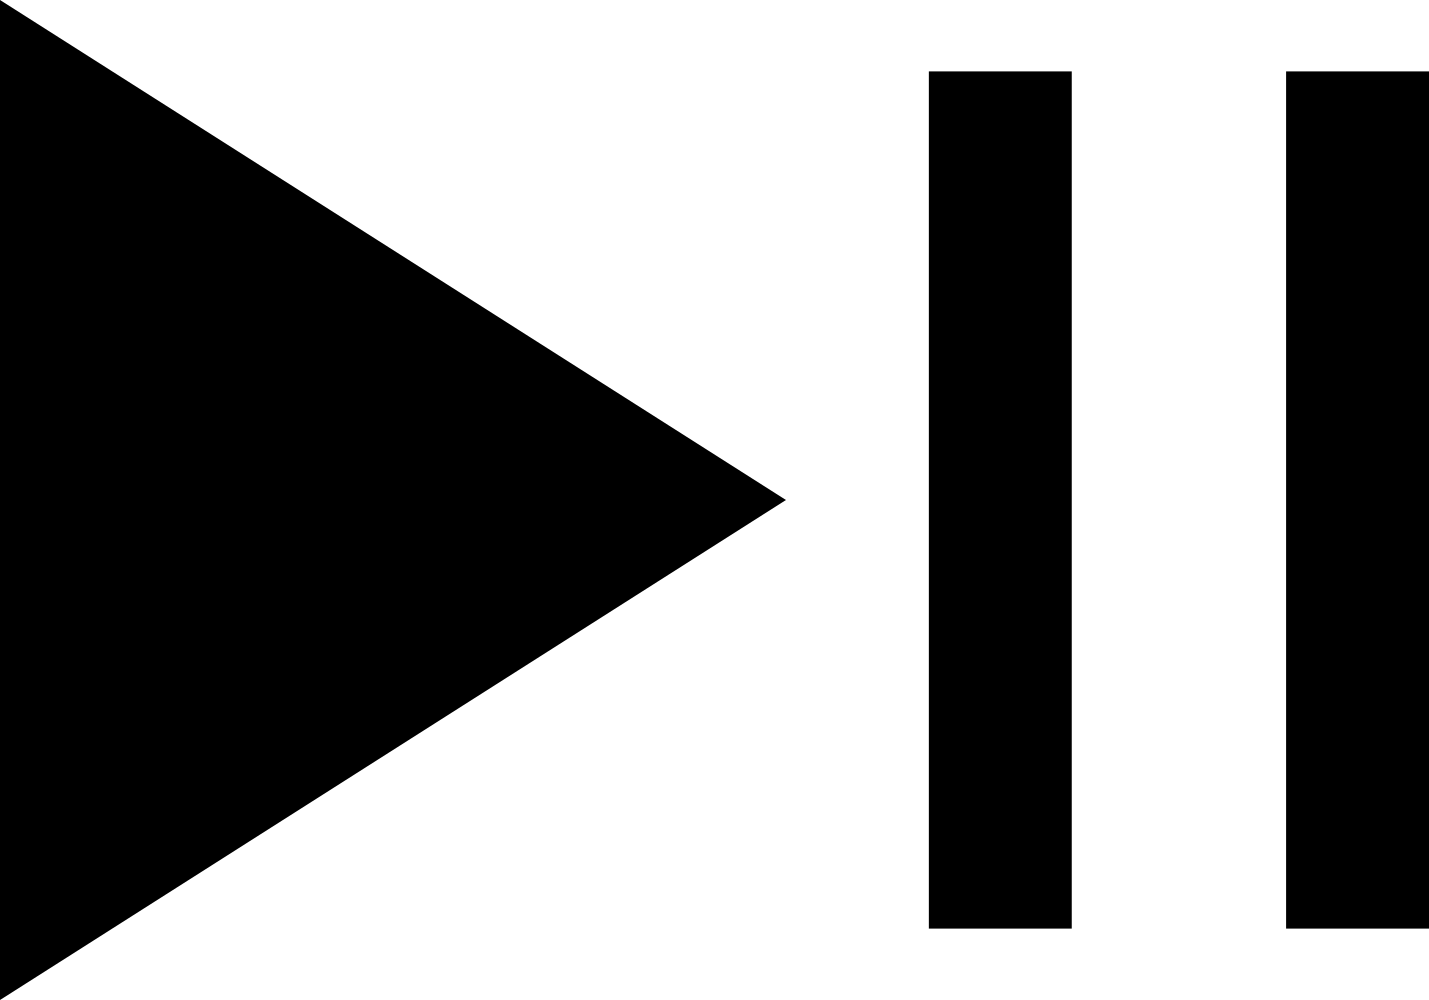
\includegraphics[height=.75\textheight]{corogfx/icon_play_pause.png}
  \end{center}

  \note{
  \begin{itemize}
    \item Function that can be paused
    \item Can be resumed later with surrounding state still intact
    \item There's three major components of the mechanism...
  \end{itemize}
  }
\end{frame}

\begin{frame}
  \frametitle{The coroutine return type}

  \begin{center}
    \tikz \draw node[pos=.5,fill=co_return_object,scale=4] {ReturnType};
  \end{center}

  \note{
  \begin{itemize}
    \item The return type is the return type of the function
    \item This is a user defined type that defines the interface through which we can interact with the coroutine
    \item Coroutines in C++ allow for a wide range of behaviors and one goal of this talk is to help us understand better what the design space for the return types looks like.
  \end{itemize}
  }
\end{frame}

\begin{frame}[fragile]
  \frametitle{Return type example}

  \begin{lstlisting}[style=cpp20]
(*@\danch(ar010)@*)CustomType(*@\danch(br010)@*) my_coroutine();
  \end{lstlisting} \
  \monobox[blue](ar010:br010) \
\
  \pause \
\
  \begin{lstlisting}[style=cpp20]
(*@\danch(ar020)@*)std::generator<int>(*@\danch(br020)@*) integer_sequence(int begin, int end) {
  for (int i = begin; i < end; ++i) { co_yield i; }
}
  \end{lstlisting} \
  \monobox[blue](ar020:br020) \
\
  \pause \
\
  \begin{lstlisting}[style=cpp20]
int main() {
  for (auto i : integer_sequence(0, 10)) {
    std::println("{}", i);
  }
}
  \end{lstlisting}

  \note{
  \begin{itemize}
    \item \alert<1>{When calling a coroutine for the first time, think of it as calling the factory function that produces the return object.}
    \item \alert<1>{Notice how we cannot tell from the signature whether the function is a coroutine. This is different to most modern coroutine implementations in other languages, as we will see later. *** TRANSITION***}
    \item \alert<2>{Since C++23 we have one coro ret type provided by the standard library: std::generator}
    \item \alert<2>{Generator allows us to yield values from the middle of a function  *** TRANSITION***}
    \item It implements the range concept, so anything that works with ranges can consume the values from the generator
    \item If you don't see how this is useful, try implementing an iterator that traverses a complex data structure like a tree or a graph. You will see it is surprisingly difficult and coroutines make it much easier.
    \item Part 1 showed everything that you need to write a generator yourself.
  \end{itemize}
  }
\end{frame}

\begin{frame}
  \frametitle{The coroutine promise}

  \begin{center}
    \tikz \draw node[pos=.5,fill=co_promise,scale=4,font=\ttfamily] {promise\_type};
  \end{center}

  \note{
  \begin{itemize}
    \item The return type determines the user facing interface, the promise is the compiler facing interface
    \item It provides means for customizing the behavior invoked during starting and shutting down the coroutine
  \end{itemize}
  }
\end{frame}

\begin{frame}[fragile]

  \frametitle{Cheat Sheet - Promise Type}

  \begin{lstlisting}[style=cpp20,numbers=left]
struct (*@\danch(ar100)@*)ReturnType(*@\danch(br100)@*) / std::coroutine_traits<(*@\danch(mr100)@*)ReturnType(*@\danch(nr100)@*), ...> { 
  struct (*@\danch(cr100)@*)promise_type(*@\danch(dr100)@*) {
    (*@\danch(kr100)@*)promise_type(T...);(*@\danch(lr100)@*)  // opt.
    (*@\danch(er100)@*)ReturnType(*@\danch(fr100)@*) get_return_object();
    (*@\danch(gr100)@*)std::suspend_always(*@\danch(hr100)@*) initial_suspend();
    // ---- (*@$\Uparrow$@*) Start / (*@$\Downarrow$@*) Shutdown ----
    void return_value(T); / void return_void();
    void unhandled_exception();
    (*@\danch(ir100)@*)std::suspend_always(*@\danch(jr100)@*) final_suspend() noexcept;
\end{lstlisting}\begin{lstlisting}[style=cpp20]
  };
};
  \end{lstlisting}

  \monobox[blue](ar100:br100)
  \monobox[blue](mr100:nr100)
  \monobox[red](cr100:dr100)
  \monobox[blue](er100:fr100)
  \monobox[green](gr100:hr100)
  \monobox[green](ir100:jr100)

  \note{
  \begin{itemize}
    \item Unlike with the return type, which we can implement however we want, the standard lays out which functions need to be provided by a promise.
    \item We implement each of those functions ourselves and the compiler will call them at the appropriate point during a coroutine's execution.
    \item Note that we won't be calling any of those functions directly from user code.
  \end{itemize}
  }
\end{frame}

\begin{frame}
  \frametitle{Awaitable}

  \begin{center}
    \tikz \draw node[pos=.5,fill=co_awaitable,scale=4] {Awaitable};
  \end{center}

  \note{
  \begin{itemize}
    \item Finally, there's the awaitable. An awaitable is a type that we can use as an argument to operator \texttt{co\_await} on, which is the operation that thriggers suspension from within a running coroutine.
  \end{itemize}
  }
\end{frame}

\begin{frame}[fragile]

  \frametitle{Cheat Sheet - Awaitable}

  \begin{lstlisting}[style=cpp20,numbers=left]
struct (*@\danch(ar101)@*)Awaitable(*@\danch(br101)@*) {
  bool await_ready();
  auto await_suspend(std::coroutine_handle<(*@\danch(cr101)@*)promise_type(*@\danch(dr101)@*)>);
  auto await_resume(); 
};
\end{lstlisting}

  \monobox[green](ar101:br101)
  \monobox[red](cr101:dr101)

  \note{
  \begin{itemize}
    \item Like the promise, this is a compiler-facing interface and will not be called from user code.
    \item The functions of the Awaitable customize what happens when a coroutine is suspended or wakes up.
  \end{itemize}
  }
\end{frame}


\begin{frame}[fragile]
  \frametitle{Cheat Sheet: Map of Coroutine Land}

  \begin{center}
  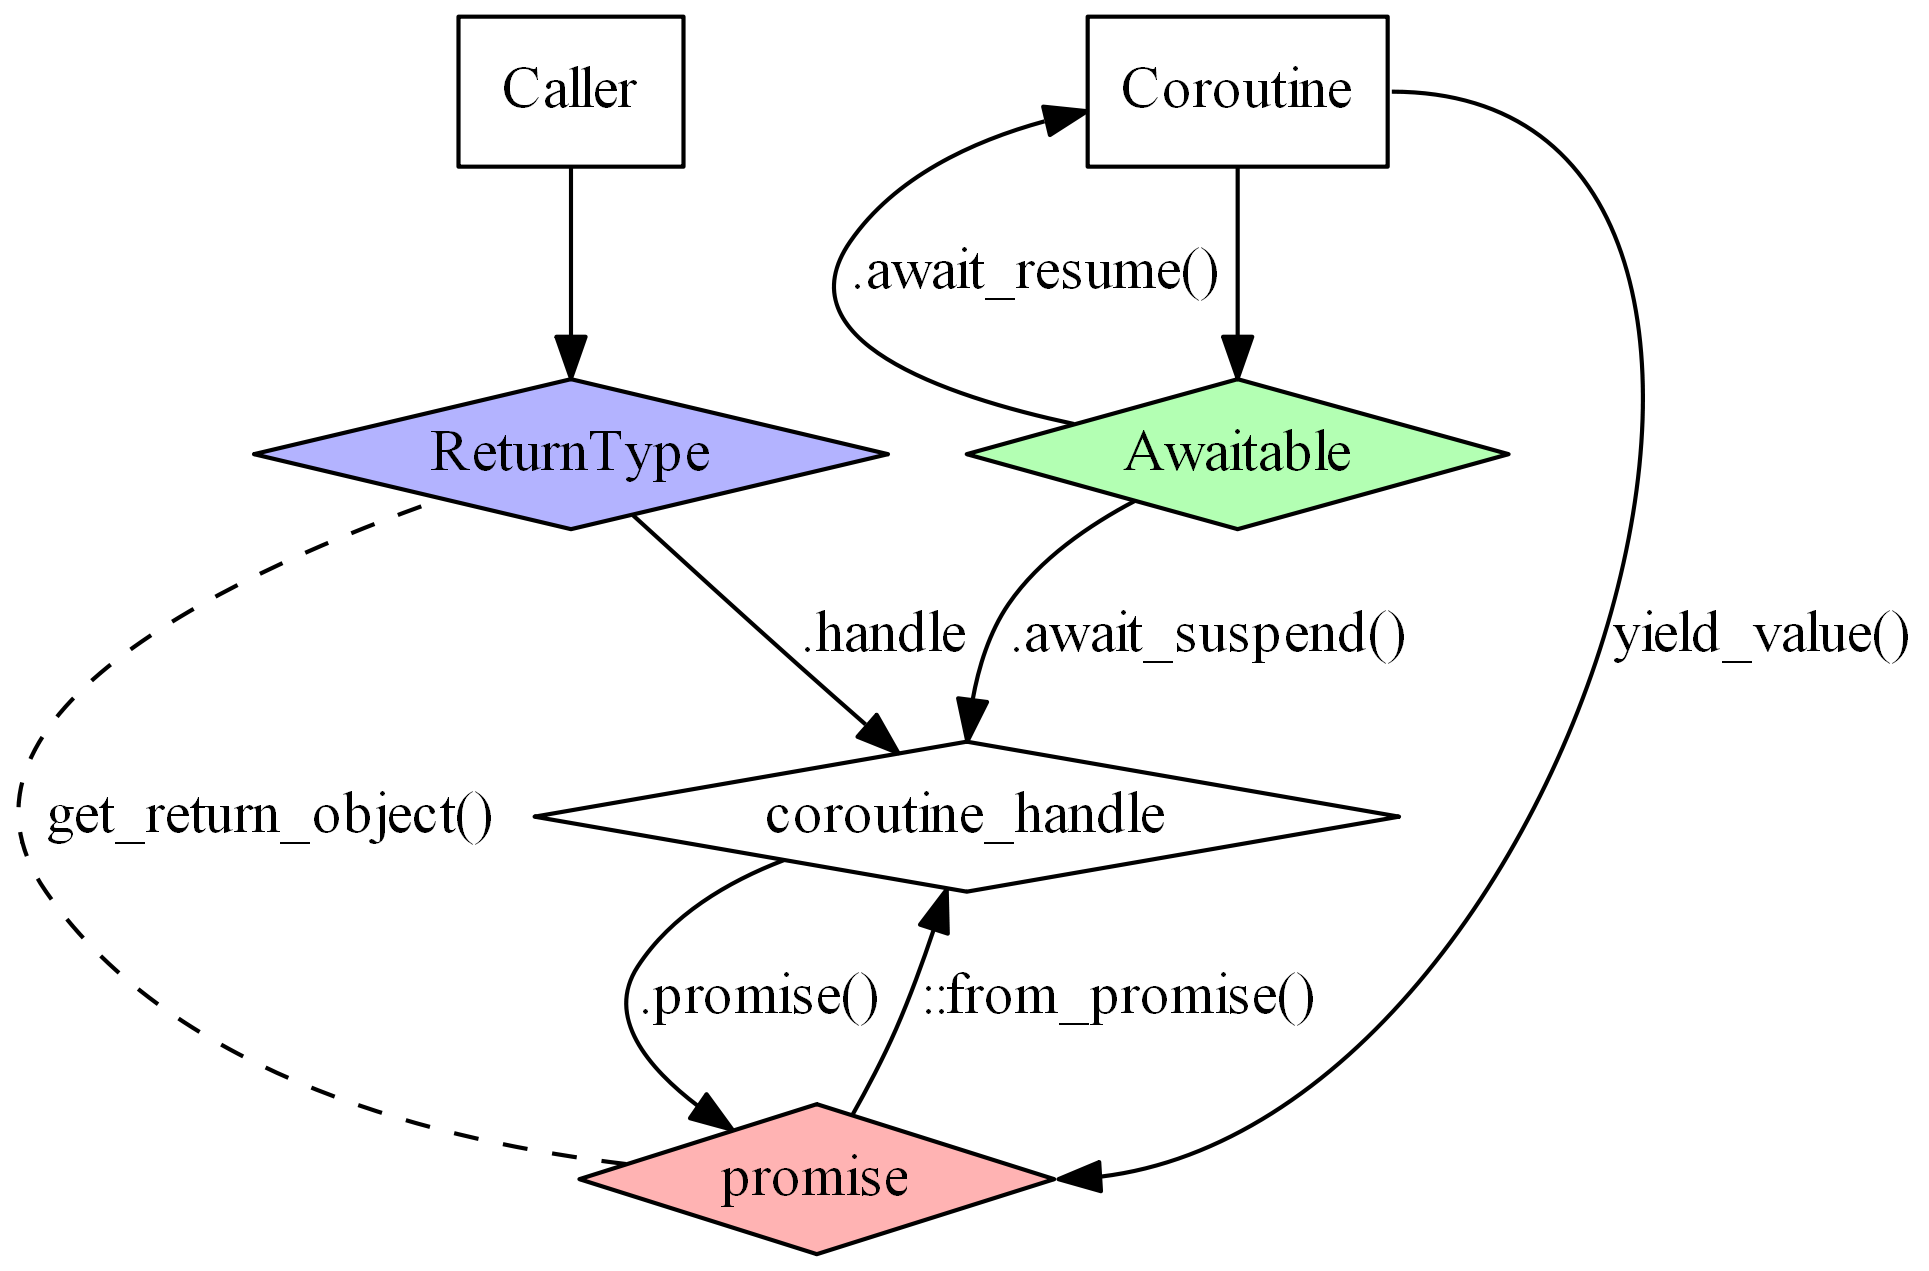
\includegraphics[height=.9\textheight]{corogfx/acquaintances05.png}
  \end{center}

  \note{
  \begin{itemize}
    \item And here we can see how these three parts are connected. We established this cheat sheet in part 1 to help us visualize how the different parts interact.
    \item In particular, note how the promise type sits at a central position between caller and coroutine context. It can be used to store data that is passed between the two.
  \end{itemize}
  }
\end{frame}

\begin{frame}[fragile]
  \frametitle{Get the cheat sheet!}
  \begin{center}
    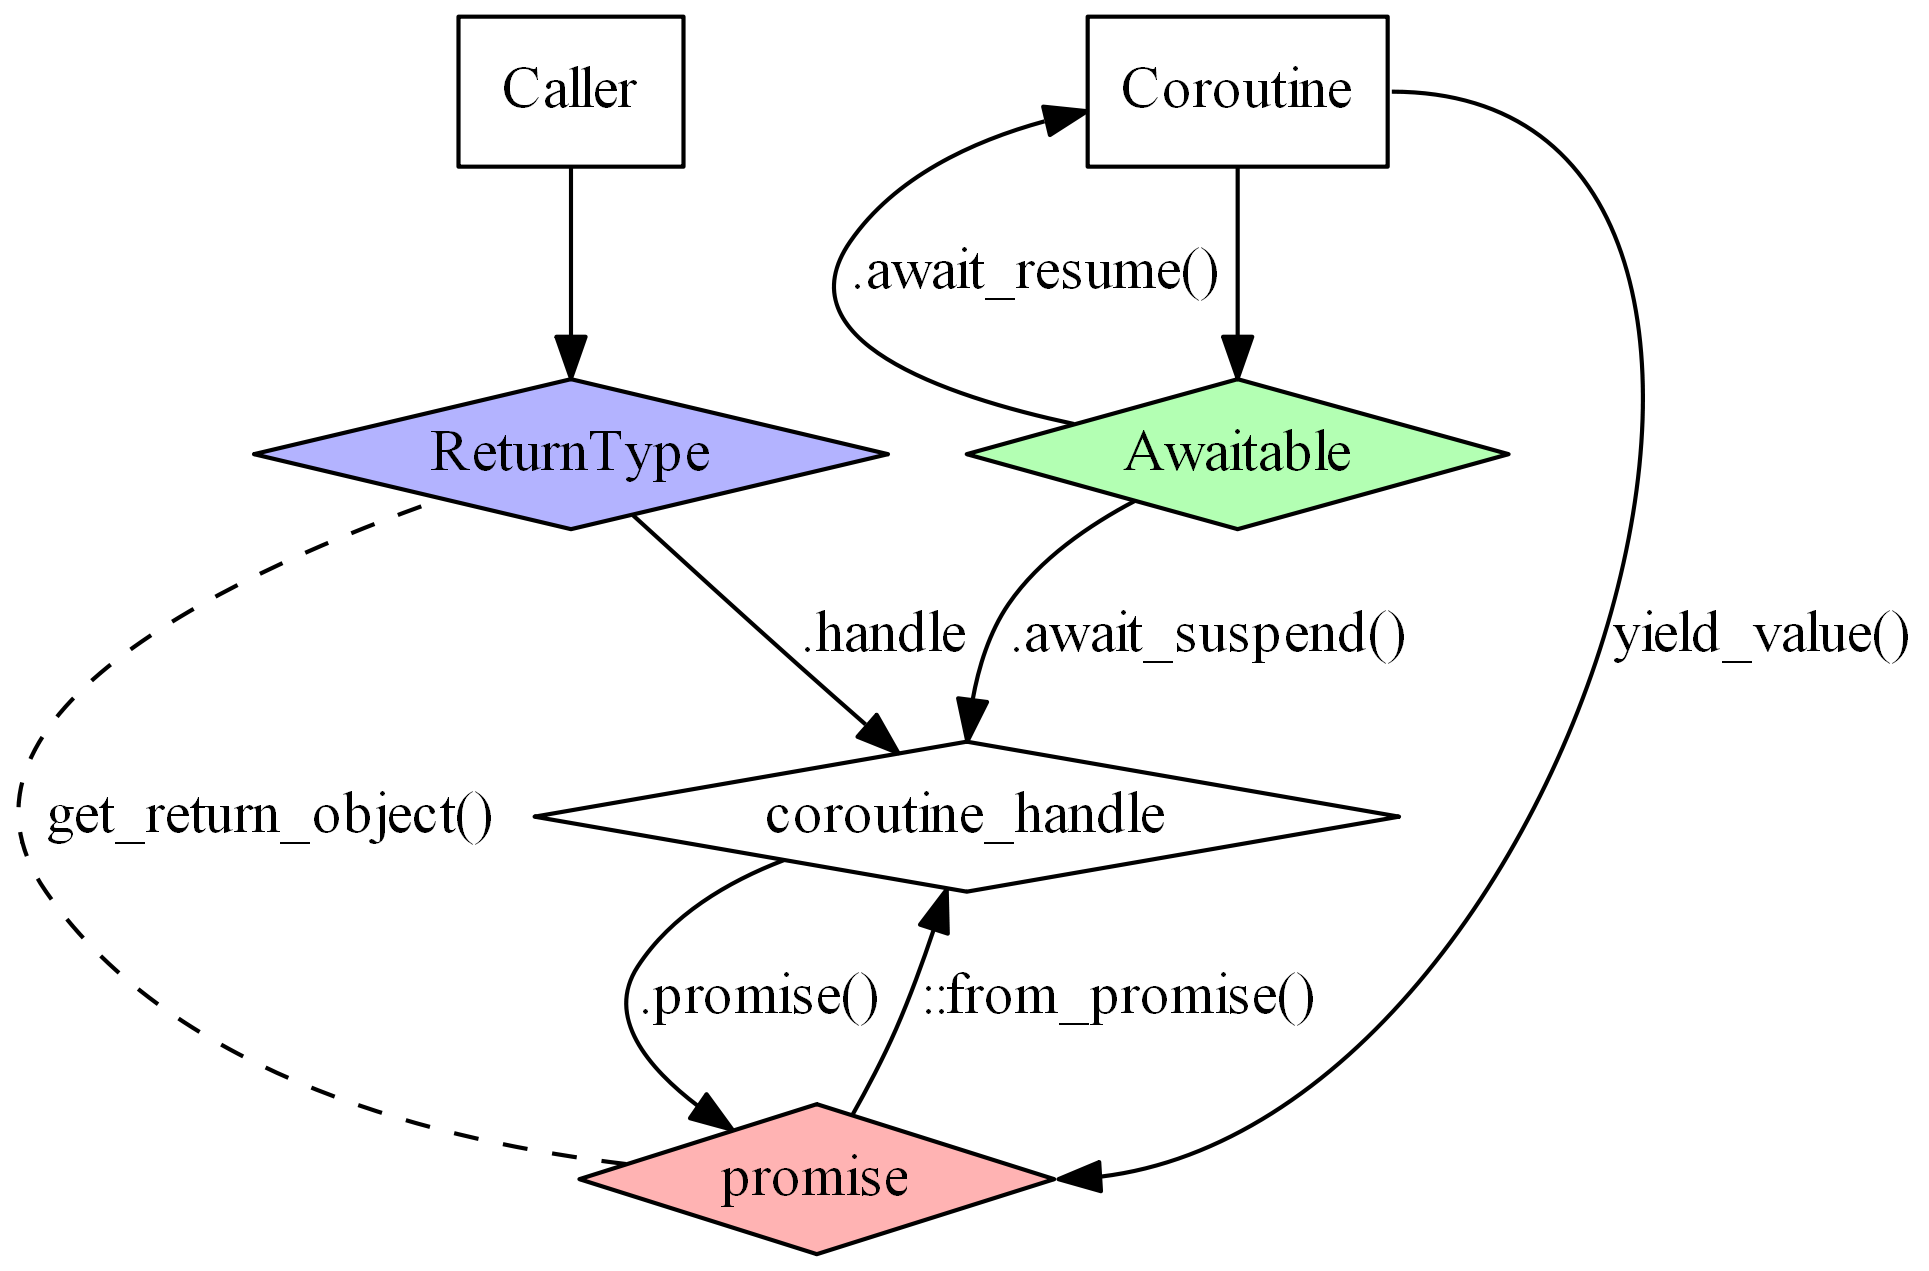
\includegraphics[height=.6\textheight]{corogfx/acquaintances05.png}
    \hspace{12ex}
    \href{https://github.com/ComicSansMS/cpp20_coroutine_cheat_sheet}{\includegraphics[height=.6\textheight]{corogfx/qrcode}}
  \end{center}
  \vspace{20em}

  \note{
  \begin{itemize}
    \item You can find a copy of the entire cheat sheet here. I will leave this up for a second to give you time to scan the QR code if you want to use the cheat sheet to follow along later.
    \item Why am I back now with a part 2? At the end of part 1 I said we now understand all of the boring parts and can start focussing on the interesting stuff.
    \item This talk is about an interesting use case that is of particular prominence, namely asynchronous computation. Other languages have dedicated language features for this. C\#, Python, Javascript, Rust, and others all have async/await. We will see in this talk how we can implement async/await with C++20 coroutines and how it behaves different from those languages.
  \end{itemize}
  }
\end{frame}

\begin{frame}
  \frametitle{Andrzej Krzemiesńki at code::dive 2023}

  \begin{center}
    \href{https://www.youtube.com/watch?v=ZSkign_3Hp4}{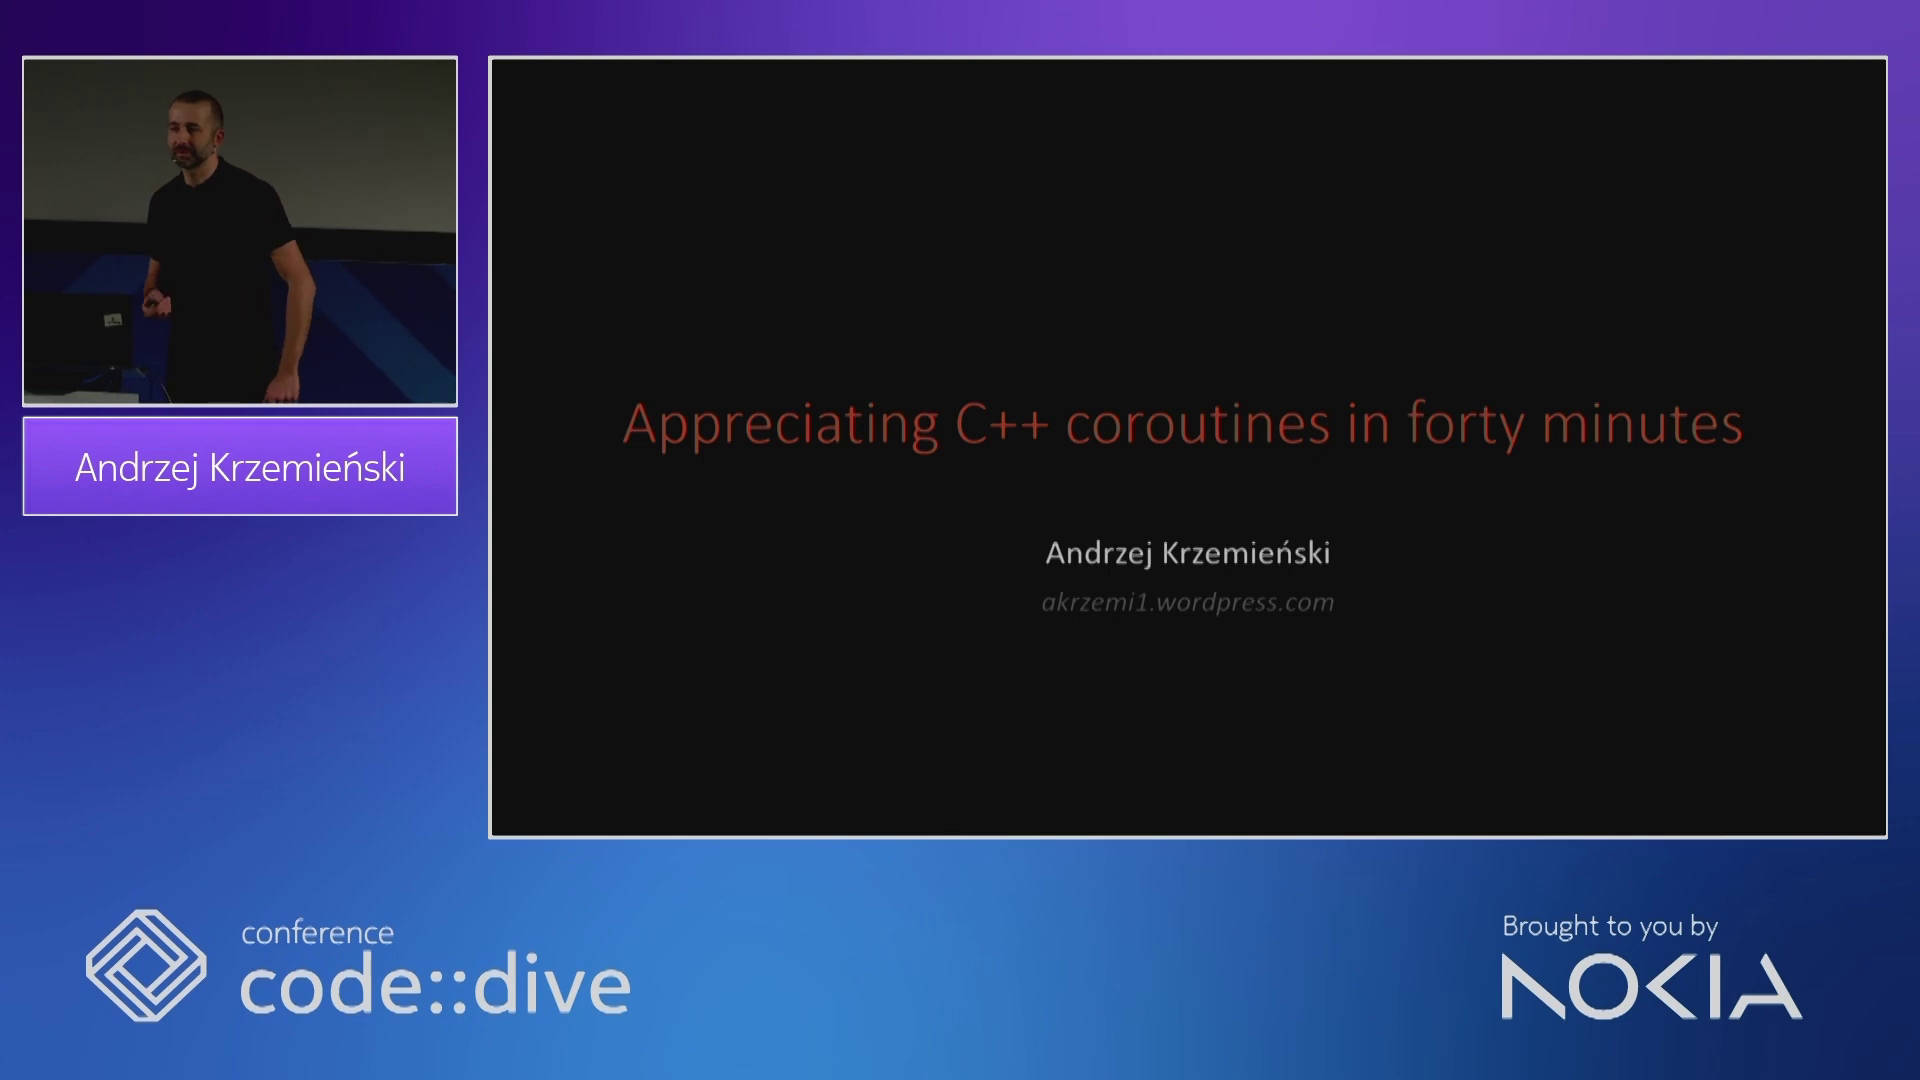
\includegraphics[height=.95\textheight]{corogfx2/talk_andrzej.jpg}}
  \end{center}

  \note{
  \begin{itemize}
  \item I will not have the time here to motivate why async/await is useful in the first place. If you don't know it from other languages and are still skeptical...
  \item Andrzej gave a great talk focusing exclusively on motivating exactly this use case for coroutines at code::dive 2023.
  \end{itemize}
  }
\end{frame}

\begin{frame}
  \frametitle{Words of caution}

  \begin{itemize}
  \item I will at times lead you astray. This is intentional and will hopefully deepen your insight.
  \vspace{20pt}
  \item We will be largely ignoring multithreading for this talk.
  \vspace{20pt}
  \item This is not a best-practice talk.
  \end{itemize}
\end{frame}

\begin{frame}[fragile]
  \frametitle{A mental model for coroutines: Cooperative Threads}

  \begin{onlyenv}<1-2>
  \begin{lstlisting}[style=cpp20]
void spawn_task() {
  // ...
  Result r = outer_function();
}
  (*@ \pause @*)
Result outer_function() {
  PartialResult r = middle_function();
  return Result::from_partial_result(r);
}
  \end{lstlisting}
  \end{onlyenv}

  \begin{onlyenv}<3-4>
  \begin{lstlisting}[style=cpp20]
PartialResult middle_function() {
  auto r = inner_function();
  return PartialResult::from_io_result(r);
}
  (*@ \pause \pause @*)
IoResult inner_function() {
  auto data = blocking_io(...); // this could take some time
  return IoResult::from_io_data(data);
}
  \end{lstlisting}
  \end{onlyenv}

  \note{ \color{green}{TIME!} \color{black}{0:05} }
\end{frame}

\begin{frame}
  \frametitle{Call Stack}

  \begin{onlyenv}<1>
  \begin{tikzpicture}[node distance = 0mm and 5mm]
    \node (main)    [stackframe]                  {main()};
    \node (spawn)   [stackframe,above=of main]    {spawn\_task()};
    \node (outer)   [stackframe,above=of spawn]   {outer\_function()};
    \node (middle)  [stackframe,above=of outer]   {middle\_function()};
    \node (inner)   [stackframe,above=of middle]  {inner\_function() 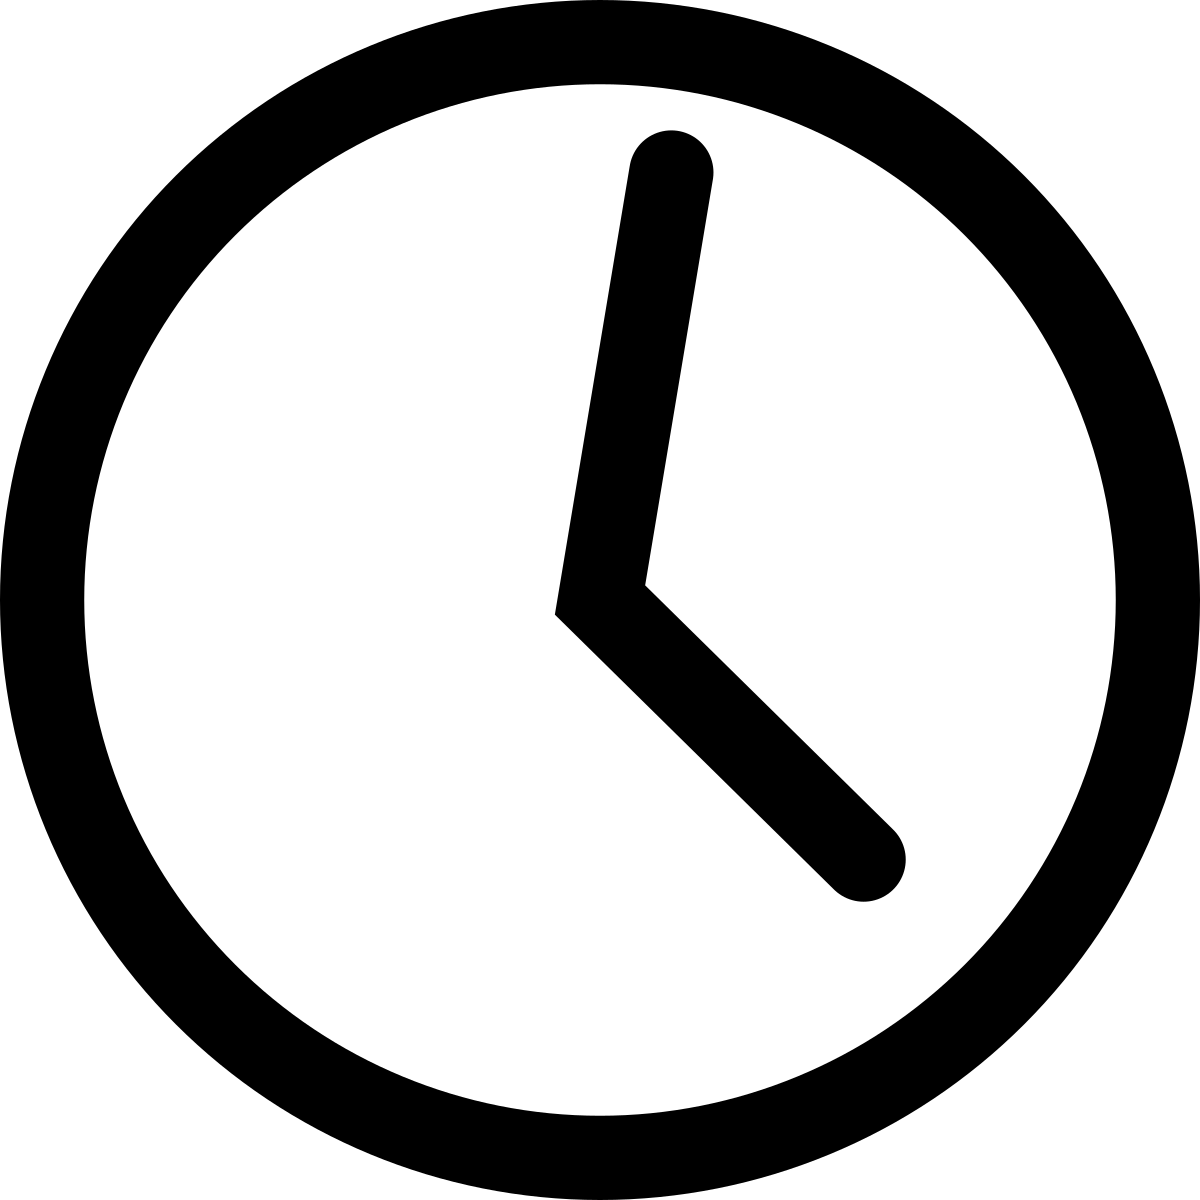
\includegraphics[height=9pt]{corogfx2/icon_clock.png}};
  \end{tikzpicture}
  \end{onlyenv}
  \begin{onlyenv}<2>
  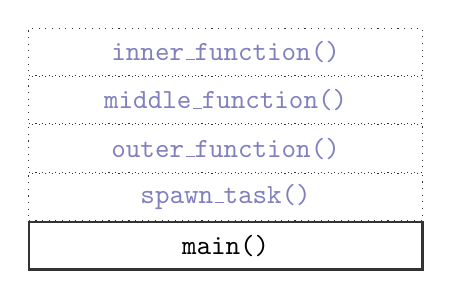
\begin{tikzpicture}[node distance = 0mm and 5mm]
    \node (main)    [stackframe]                  {main()};
    \node (spawn)   [suspended,above=of main]    {spawn\_task()};
    \node (outer)   [suspended,above=of spawn]   {outer\_function()};
    \node (middle)  [suspended,above=of outer]   {middle\_function()};
    \node (inner)   [suspended,above=of middle]  {inner\_function()};
  \end{tikzpicture}
  \end{onlyenv}

  \begin{onlyenv}<3>
  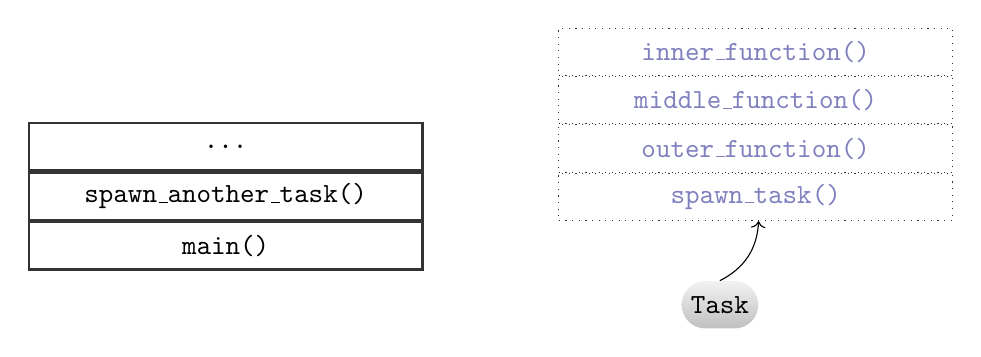
\begin{tikzpicture}[node distance = 0mm and 5mm]
    \node (main)    [stackframe]                       {main()};
    \node (other)   [stackframe,above=of main]         {spawn\_another\_task()};
    \node (other2)  [stackframe,above=of other]        {...};

    \node (spawn)   [suspended,above right=of main,shift={(8ex,0)}]    {spawn\_task()};
    \node (outer)   [suspended,above=of spawn]         {outer\_function()};
    \node (middle)  [suspended,above=of outer]         {middle\_function()};
    \node (inner)   [suspended,above=of middle]        {inner\_function()};

    \node(task)     [taskobj,below=of spawn,shift={(-3ex,-5ex)}] {Task};
    \path (task.north) edge[->,bend right] (spawn);
  \end{tikzpicture}
  \end{onlyenv}

  \note{
  \begin{itemize}
  \item \alert<+>{Blocking I/O will prevent program from doing useful work.}
  \item ***TRANSITION***
  \item \alert<+>{Main thread can not do any useful while we are waiting. But what if we could suspend them...}
  \item ***TRANSITION***
  \item And do useful stuff instead of just wait. We associate the suspended tasks with an object so that we can get back to them later.
  \end{itemize}
  }
\end{frame}

\begin{frame}[fragile]
  \frametitle{Threads - A straightforward solution}

  \begin{onlyenv}<1>
  \begin{lstlisting}[style=cpp20]
std::future<Result> spawn_task() {
  return std::async(outer_function);
}
  \end{lstlisting}
  \end{onlyenv}

  \begin{onlyenv}<2>
  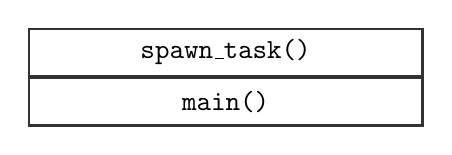
\begin{tikzpicture}[node distance = 0mm and 5mm]
    \node (main)    [stackframe]                       {main()};
    \node (other)   [stackframe,above=of main]         {spawn\_task()};
  \end{tikzpicture}
  \end{onlyenv}

  \begin{onlyenv}<3>
  \begin{tikzpicture}[node distance = 0mm and 5mm]
    \node (main)    [stackframe]                       {main()};
    \node (other2)  [stackframe,above=of main]        {...};

    \node (spawn)   [stackframe,above right=of main,shift={(8ex,0)}]    {\_\_thread\_main()};
    \node (outer)   [stackframe,above=of spawn]         {outer\_function()};
    \node (middle)  [stackframe,above=of outer]         {middle\_function()};
    \node (inner)   [stackframe,above=of middle]        {inner\_function() 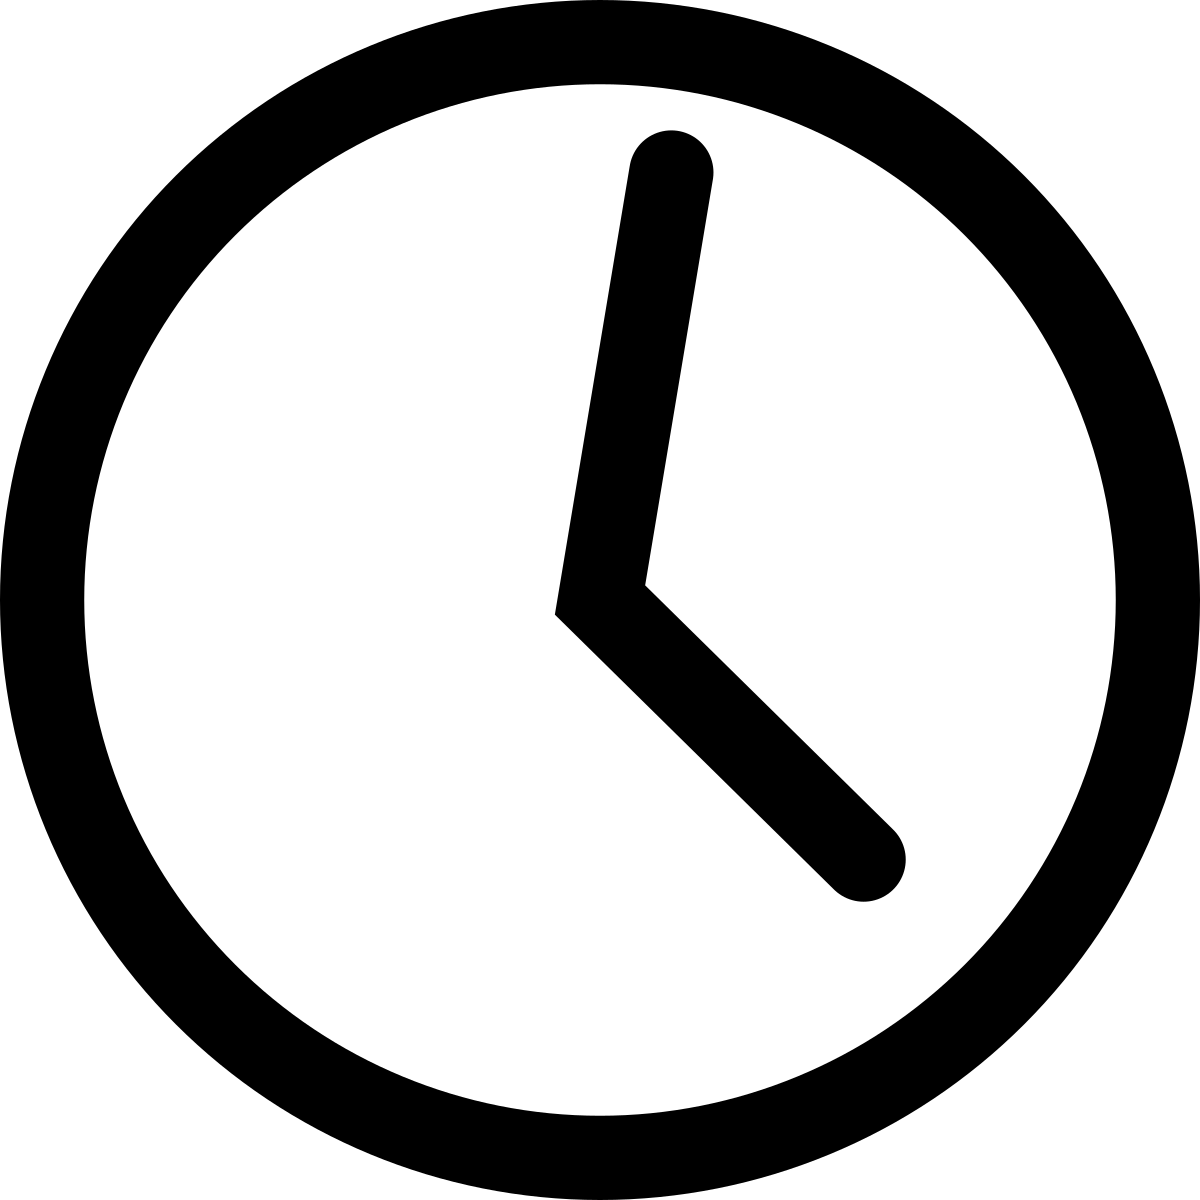
\includegraphics[height=9pt]{corogfx2/icon_clock.png}};

    \node(task)     [taskobj,below=of spawn,shift={(-3ex,-5ex)}] {std::future<Result>};
    \path (task) edge[->,bend right] (spawn);
  \end{tikzpicture}
  \end{onlyenv}
\end{frame}


\begin{frame}
  \frametitle{Threads - Evaluation}

  \cpause
  \begin{itemize}
  \item Thread creation is CPU and memory intensive \cpause
  \item Thread switching is expensive \cpause
  \item Blocked threads may still consume CPU cycles! \cpause
  \item Shared data must be synchronized correctly. \cpause
  \item ... \cpause
  \end{itemize}

  Not a solution that scales well.

  Can be a good solution for small number of tasks.
\end{frame}

\begin{frame}[fragile]
  \frametitle{Green Threads aka Stackful Coroutines}

  \begin{onlyenv}<1-2>
  \begin{lstlisting}[style=cpp20]
auto spawn_task() {
  return spawn_green_thread(outer_function);
} (*@ \cpause @*)

IoResult inner_function() {
  auto request = setup_non_blocking_io(...);
  this_green_thread::suspend_waiting_for(request);
  auto data = retrieve_io_data(request);
  return IoResult::from_io_data(data);
}
  \end{lstlisting}
  \end{onlyenv}

  \note{
  \begin{itemize}
  \item \alert<+>{aka Fibers, aka User-mode Threads, aka Cooperative MT}
  \item ***TRANSITION*** inner function suspends
  \end{itemize}
  }
\end{frame}

\begin{frame}
  \frametitle{Green Threads aka Stackful Coroutines}
  
  \begin{onlyenv}<1>
  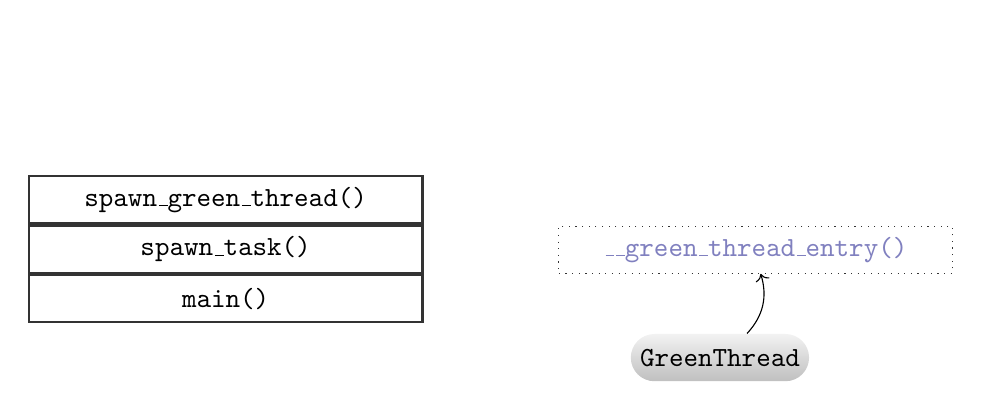
\begin{tikzpicture}[node distance = 0mm and 5mm]
    \node (main)    [stackframe]                  {main()};
    \node (spawn)   [stackframe,above=of main]    {spawn\_task()};
    \node (spawn2)   [stackframe,above=of spawn]  {spawn\_green\_thread()};
    
    \node (spawn)   [suspended,above right=of main,shift={(8ex,0)}]    {\_\_green\_thread\_entry()};
    \node (place)   [stackframe,above=of spawn,style={draw=white}]   {};
    \node (place2)   [stackframe,above=of place,style={draw=white}]   {};
    \node (place3)   [stackframe,above=of place2,style={draw=white}]   {};
    \node (place4)   [stackframe,above=of place3,style={draw=white}]   {};

    \node(task)     [taskobj,below=of spawn,shift={(-3ex,-5ex)}] {GreenThread};
    \path (task) edge[->,bend right] (spawn);
  \end{tikzpicture}
  \end{onlyenv}
  
  \begin{onlyenv}<2-3>
  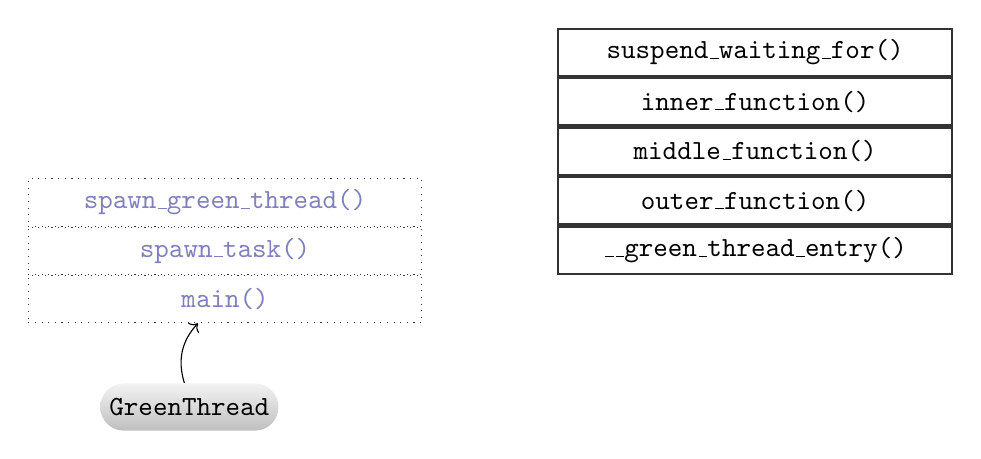
\begin{tikzpicture}[node distance = 0mm and 5mm]
    \node (main)    [suspended]                  {main()};
    \node (spawn)   [suspended,above=of main]    {spawn\_task()};
    \node (spawn2)   [suspended,above=of spawn]  {spawn\_green\_thread()};
    
    \node (spawn)   [stackframe,above right=of main,shift={(8ex,0)}]    {\_\_green\_thread\_entry()};
    \node (outer)   [stackframe,above=of spawn] {outer\_function()};
    \node (middle)  [stackframe,above=of outer]   {middle\_function()};
    \node (inner)   [stackframe,above=of middle]  {inner\_function()};
    \node (place)   [stackframe,above=of inner,style={draw=white}]   {};
    \only<3>{
    \node (inner2)   [stackframe,above=of inner]  {suspend\_waiting\_for()};
    }

    \node(task)     [taskobj,below=of main,shift={(-3ex,-5ex)}] {GreenThread};
    \path (task) edge[->,bend left] (main);
  \end{tikzpicture}
  \end{onlyenv}
  
  \begin{onlyenv}<4>
  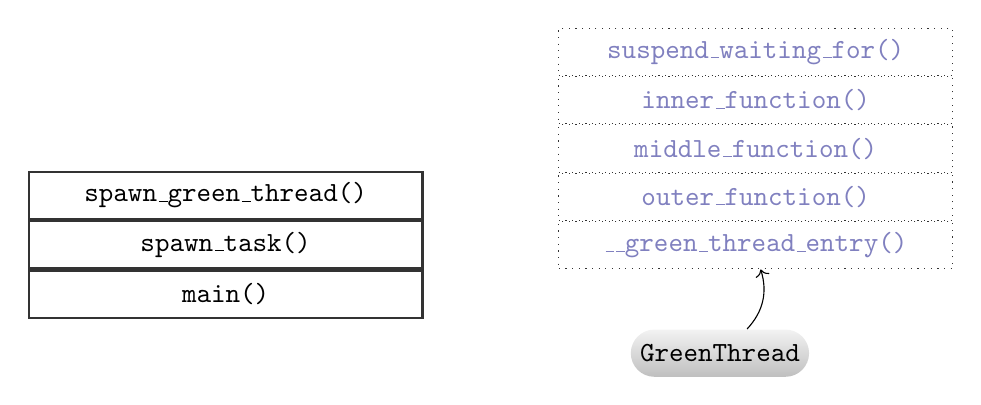
\begin{tikzpicture}[node distance = 0mm and 5mm]
    \node (main)    [stackframe]                  {main()};
    \node (spawn)   [stackframe,above=of main]    {spawn\_task()};
    \node (spawn2)   [stackframe,above=of spawn]  {spawn\_green\_thread()};
    
    \node (spawn)   [suspended,above right=of main,shift={(8ex,0)}]    {\_\_green\_thread\_entry()};
    \node (outer)   [suspended,above=of spawn] {outer\_function()};
    \node (middle)  [suspended,above=of outer]   {middle\_function()};
    \node (inner)   [suspended,above=of middle]  {inner\_function()};
    \node (inner2)   [suspended,above=of inner]  {suspend\_waiting\_for()};

    \node(task)     [taskobj,below=of spawn,shift={(-3ex,-5ex)}] {GreenThread};
    \path (task) edge[->,bend right] (spawn);
  \end{tikzpicture}
  \end{onlyenv}
  
  \begin{onlyenv}<5>
  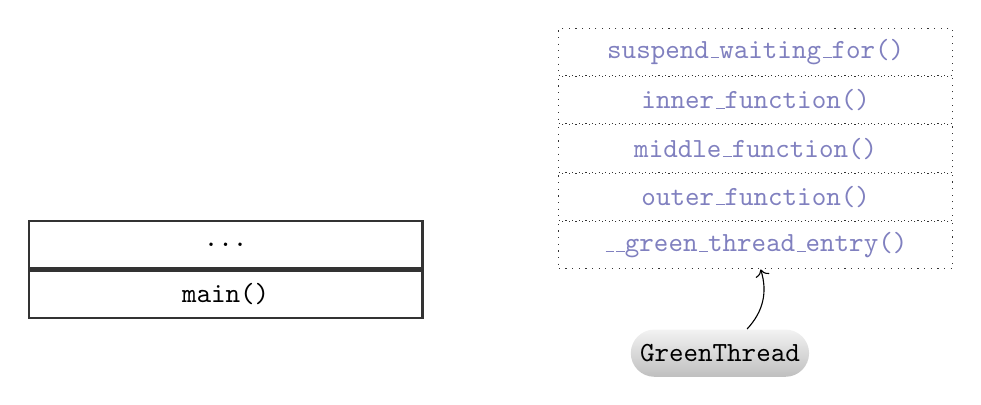
\begin{tikzpicture}[node distance = 0mm and 5mm]
    \node (main)    [stackframe]                  {main()};
    \node (spawn)   [stackframe,above=of main]    {...};
    \node (spawn2)   [stackframe,above=of spawn,style={draw=white}]  {};
    
    \node (spawn)   [suspended,above right=of main,shift={(8ex,0)}]    {\_\_green\_thread\_entry()};
    \node (outer)   [suspended,above=of spawn] {outer\_function()};
    \node (middle)  [suspended,above=of outer]   {middle\_function()};
    \node (inner)   [suspended,above=of middle]  {inner\_function()};
    \node (inner2)   [suspended,above=of inner]  {suspend\_waiting\_for()};

    \node(task)     [taskobj,below=of spawn,shift={(-3ex,-5ex)}] {GreenThread};
    \path (task) edge[->,bend right] (spawn);
  \end{tikzpicture}
  \end{onlyenv}
  
  \begin{onlyenv}<6>
  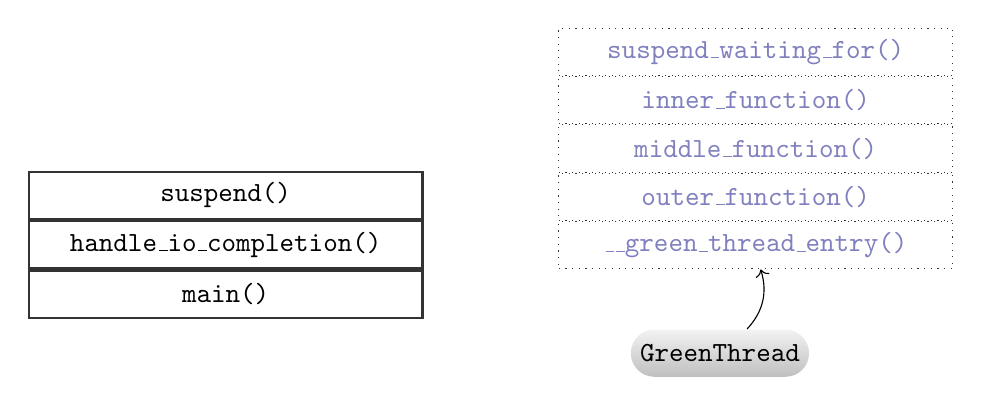
\begin{tikzpicture}[node distance = 0mm and 5mm]
    \node (main)    [stackframe]                  {main()};
    \node (spawn)   [stackframe,above=of main]    {handle\_io\_completion()};
    \node (spawn2)   [stackframe,above=of spawn]  {suspend()};
    
    \node (spawn)   [suspended,above right=of main,shift={(8ex,0)}]    {\_\_green\_thread\_entry()};
    \node (outer)   [suspended,above=of spawn] {outer\_function()};
    \node (middle)  [suspended,above=of outer]   {middle\_function()};
    \node (inner)   [suspended,above=of middle]  {inner\_function()};
    \node (inner2)   [suspended,above=of inner]  {suspend\_waiting\_for()};

    \node(task)     [taskobj,below=of spawn,shift={(-3ex,-5ex)}] {GreenThread};
    \path (task) edge[->,bend right] (spawn);
  \end{tikzpicture}
  \end{onlyenv}
  
  \begin{onlyenv}<7>
  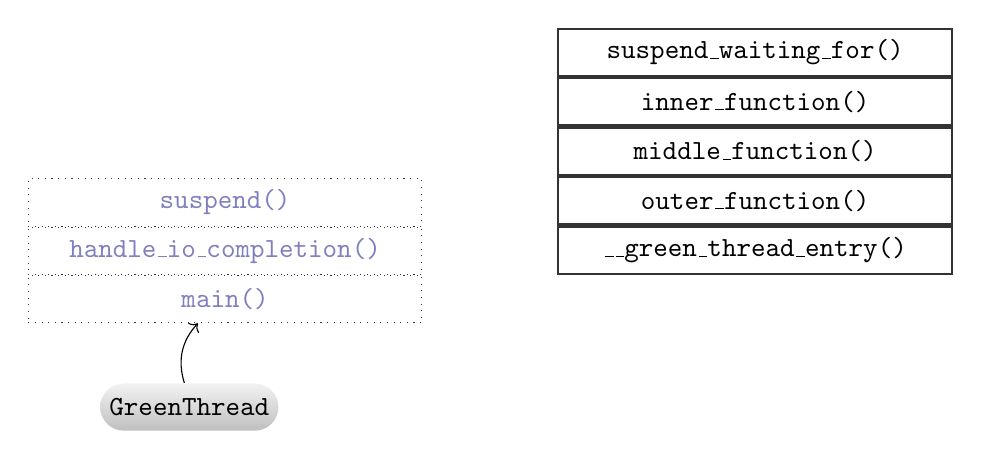
\begin{tikzpicture}[node distance = 0mm and 5mm]
    \node (main)    [suspended]                  {main()};
    \node (spawn)   [suspended,above=of main]    {handle\_io\_completion()};
    \node (spawn2)   [suspended,above=of spawn]  {suspend()};
    
    \node (spawn)   [stackframe,above right=of main,shift={(8ex,0)}]    {\_\_green\_thread\_entry()};
    \node (outer)   [stackframe,above=of spawn] {outer\_function()};
    \node (middle)  [stackframe,above=of outer]   {middle\_function()};
    \node (inner)   [stackframe,above=of middle]  {inner\_function()};
    \node (inner2)   [stackframe,above=of inner]  {suspend\_waiting\_for()};

    \node(task)     [taskobj,below=of main,shift={(-3ex,-5ex)}] {GreenThread};
    \path (task) edge[->,bend left] (main);
  \end{tikzpicture}
  \end{onlyenv}
  
  \begin{onlyenv}<8>
  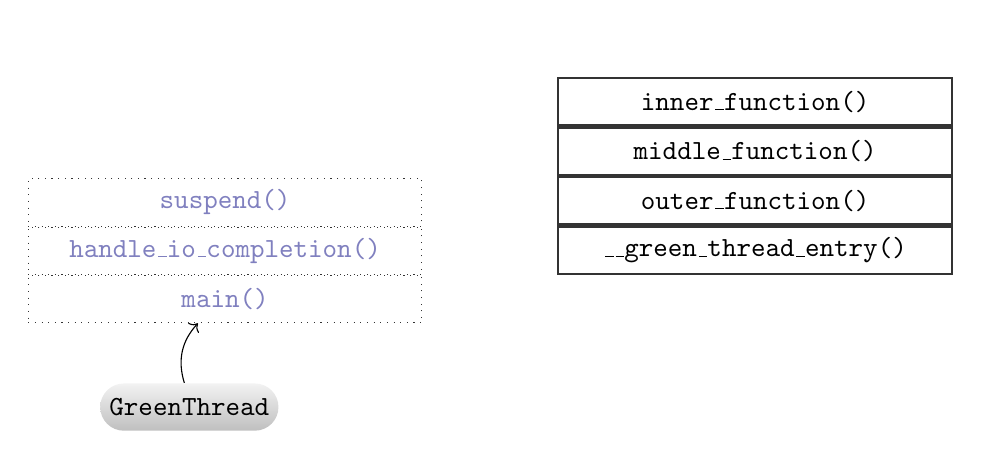
\begin{tikzpicture}[node distance = 0mm and 5mm]
    \node (main)    [suspended]                  {main()};
    \node (spawn)   [suspended,above=of main]    {handle\_io\_completion()};
    \node (spawn2)   [suspended,above=of spawn]  {suspend()};
    
    \node (spawn)   [stackframe,above right=of main,shift={(8ex,0)}]    {\_\_green\_thread\_entry()};
    \node (outer)   [stackframe,above=of spawn] {outer\_function()};
    \node (middle)  [stackframe,above=of outer]   {middle\_function()};
    \node (inner)   [stackframe,above=of middle]  {inner\_function()};
    \node (inner2)   [stackframe,above=of inner,style={draw=white}]  {};

    \node(task)     [taskobj,below=of main,shift={(-3ex,-5ex)}] {GreenThread};
    \path (task) edge[->,bend left] (main);
  \end{tikzpicture}
  \end{onlyenv}

  \note{
  \begin{itemize}
  \item \alert<+>{***TRANSITION*** task call stack}
  \item \alert<+>{***TRANSITION*** after spawning, main suspends and outer starts executing}
  \item \alert<+>{***TRANSITION*** eventually hits suspend}
  \item \alert<+>{***TRANSITION*** main calls resume}
  \item \alert<+>{***TRANSITION*** main will do other things}
  \item \alert<+>{***TRANSITION*** when io is available, main will suspend}
  \item \alert<+>{***TRANSITION*** green thread resumed}
  \item ***TRANSITION*** and continues execution
  \item All of this happens on a single OS thread!
  \end{itemize}
  }
\end{frame}


\begin{frame}
  \frametitle{Green Threads - Evaluation}

  \begin{itemize}
  \item Little overhead \cpause
  \item No synchronization needed. \cpause
  \item Green Threads cooperatively decide when to suspend and resume \cpause
  \item Intuition about control-flow is still very similar to threads
  \end{itemize}
\end{frame}


\begin{frame}
  \frametitle{C++20 Coroutines}

  \begin{itemize}
  \item Stackless
  \cpause
  \item \alert{Goal: Suspend execution context larger than a single function}
  \end{itemize}
  \note{
  \color{green}{TIME!} \color{black}{0:10}
  Can we implement something like this with C++ coroutines?
  \begin{itemize}
  \item We can only suspend one function at a time
  \item If we want to suspend a computation spanning multiple functions, we need to suspend them all one by one
  \item ***TRANSITION*** goal for the talk: suspend whole execution context
  \end{itemize}
  }
\end{frame}


\begin{frame}
  \frametitle{Roadmap}
  \begin{todolist}
  \item Spawn outermost coroutine \cpause
  \item[\done] Call nested coroutines \cpause
  \item \alert<6>{Suspend entire coroutine stack} \cpause
  \item Resume entire coroutine stack \cpause
  \item Deliver final result
  \end{todolist}
\end{frame}

\begin{frame}[fragile]
  \frametitle{Suspending nested coroutines}

    \begin{onlyenv}<1>
  \begin{lstlisting}[style=cpp20]
IoResult inner_function() {
  auto data = blocking_io(...);
  return IoResult::from_io_data(data);
}
  \end{lstlisting}
  \end{onlyenv}
  \begin{onlyenv}<2>
  \begin{lstlisting}[style=cpp20]
IoResult inner_function() {
  auto data = co_await async_io(...);
  co_return IoResult::from_io_data(data);
}
  \end{lstlisting}
  \end{onlyenv}
  \begin{onlyenv}<3->
  \begin{lstlisting}[style=cpp20]
(*@\danch(ar200)@*)Async<IoResult>(*@\danch(br200)@*) inner_function() {
  auto data = co_await async_io(...);
  co_return IoResult::from_io_data(data);
}
  \end{lstlisting}
  \monobox[blue](ar200:br200)
  \end{onlyenv}

  \vspace{20pt}
  % Checkmark
  \only<4>{ \tikz\fill[fill=red!40!green!100](0,.35) -- (.25,0) -- (1,.7) -- (.25,.15) -- cycle; }

  \note{
  \textit{Introduce coroutine primitives}
  \begin{itemize}
  \item \alert<+>{starting from the inner function we had before...}
  \item \alert<+>{***TRANSITION*** add co\_await/co\_return}
  \item \alert<+>{ ***TRANSITION*** return type now becomes coroutine return type; This is often known as Task or Lazy; I call it async because async/await; There is a design space for these types}
  \item ***TRANSITION*** nothing more to do at this level
  \end{itemize}
  }
\end{frame}

\begin{frame}[fragile]
  \frametitle{Moving up the stack}

  \begin{lstlisting}[style=cpp20]
(*@\danch(ar210)@*)Async<IoResult>(*@\danch(br210)@*) inner_function();
  \end{lstlisting}
  \monobox[blue](ar210:br210)

  \begin{onlyenv}<1>
  \begin{lstlisting}[style=cpp20]
PartialResult middle_function() {
  auto r = inner_function();
  return PartialResult::from_io_result(r);
}
  \end{lstlisting}
  \end{onlyenv}
  \begin{onlyenv}<2>
  \begin{lstlisting}[style=cpp20]
(*@\danch(ar211)@*)Async<PartialResult>(*@\danch(br211)@*) middle_function() {
  auto r = co_await inner_function();
  co_return PartialResult::from_io_result(r);
}
  \end{lstlisting}
  \monobox[blue](ar211:br211)
  \end{onlyenv}
  \begin{onlyenv}<3-4>
  \begin{lstlisting}[style=cpp20]
(*@\danch(ar212)@*)Async<PartialResult>(*@\danch(br212)@*) middle_function() {
  (*@\danch(ar213)@*)Async<IoResult>(*@\danch(br213)@*) awaitable = inner_function();
  auto r = co_await awaitable;
  co_return PartialResult::from_io_result(r);
}
  \end{lstlisting}
  \monobox[blue](ar212:br212)
  \only<4>{\monobox[green](ar213:br213)}
  \end{onlyenv}

  \note{
  \textit{Motivating Async dual role}
  \begin{itemize}
  \item \alert<+>{one level up the call stack}
  \item \alert<+>{***TRANSITION*** again, co\_await + change return type; let's zoom in on the call to inner}
  \item \alert<+>{***TRANSITION*** co\_await actually awaits on the Async returned from inner}
  \item ***TRANSITION*** Async plays two roles now
  \end{itemize}
  }
\end{frame}

\begin{frame}
  \frametitle{Async has two roles to play}

  \begin{center}
    \tikz[baseline,inner sep=0]\node[anchor=base](ar2010){}; \tikz \draw node[pos=.5,scale=4,anchor=base]{Async$<>$}; \tikz[baseline,inner sep=0]\node[anchor=base](br2010){};
  \end{center}

  \tikz[overlay]\filldraw[green, opacity=0.3]
  ([shift={(0,14ex)}]br2010.center)
    -- ([shift={(0,0)}]ar2010.center)
    -- ([shift={(0,0)}]br2010.center)
    -- cycle
    ;
  \tikz[overlay]\filldraw[blue, opacity=0.3]
  ([shift={(0,14ex)}]ar2010.center)
    -- ([shift={(0,0)}]ar2010.center)
    -- ([shift={(0,14ex)}]br2010.center)
    -- cycle
    ;
\end{frame}

\begin{frame}
  \frametitle{Roadmap}
  \begin{todolist}
  \item Spawn outermost coroutine
  \item[\done] Call nested coroutines
  \only<1>{\item \alert{Suspend entire coroutine stack}}
  \only<2->{\item[\done] Suspend entire coroutine stack}
  \item \alert<3>{Resume entire coroutine stack}
  \item Deliver final result
  \end{todolist}
\end{frame}

\begin{frame}[fragile]
  \frametitle{Resuming}

  \begin{lstlisting}[style=cpp20]
(*@\danch(ar221)@*)Async<IoResult>(*@\danch(br221)@*) inner_function();
(*@\danch(ar222)@*)Async<PartialResult>(*@\danch(br222)@*) middle_function();
(*@\danch(ar223)@*)Async<Result>(*@\danch(br223)@*) outer_function();
  \end{lstlisting}
  \mixedbox(ar221:br221)
  \mixedbox(ar222:br222)
  \mixedbox(ar223:br223)
  \cpause
  \begin{lstlisting}[style=cpp20]
int main() {
(*@\danch(ar226)@*)  (*@\danch(ar225)@*)Async<Result>(*@\danch(br225)@*) r = outer_function();
(*@\danch(ar227)@*)  // ...
(*@\danch(ar228)@*)  r.resume_computation();
(*@\danch(ar229)@*)  Result result = r.get_result();
}
  \end{lstlisting}
  \monobox[blue](ar225:br225)

  \only<3-8>{\tikz[transform shape,overlay] \draw[>=triangle 45,->,darkred,very thick] ([shift={(-1em,0.25em)}]ar226.north) -- ([shift={(1em,0.25em)}]ar226.north);}
  \only<9>{\tikz[transform shape,overlay] \draw[>=triangle 45,->,darkred,very thick] ([shift={(-1em,0.25em)}]ar227.north) -- ([shift={(1em,0.25em)}]ar227.north);}
  \only<10->{\tikz[transform shape,overlay] \draw[>=triangle 45,->,darkred,very thick] ([shift={(-1em,0.25em)}]ar228.north) -- ([shift={(1em,0.25em)}]ar228.north);}

  \begin{onlyenv}<3>
  \resizebox{.008\textwidth}{!}{%
  \begin{tikzpicture}[node distance = 0mm and 5mm,overlay]
    \node at([shift={(82ex,20ex)}]0,0) (main) [stackframe]  {main()};
    \node (outer)   [stackframe,above=of main]              {outer\_function()};
    \node (middle)  [stackframe,above=of outer]             {middle\_function()};
    \node (inner)   [suspended,above=of middle]            {inner\_function()};
  \end{tikzpicture}
  }
  \end{onlyenv}
  \begin{onlyenv}<4>
  \resizebox{.008\textwidth}{!}{%
  \begin{tikzpicture}[node distance = 0mm and 5mm,overlay]
    \node at([shift={(82ex,20ex)}]0,0) (main) [stackframe]  {main()};
    \node (outer)   [stackframe,above=of main]              {outer\_function()};
    \node (middle)  [stackframe,above=of outer]             {middle\_function()};
  \end{tikzpicture}
  }
  \end{onlyenv}
  \begin{onlyenv}<5>
  \resizebox{.008\textwidth}{!}{%
  \begin{tikzpicture}[node distance = 0mm and 5mm,overlay]
    \node at([shift={(82ex,20ex)}]0,0) (main) [stackframe]  {main()};
    \node (outer)   [stackframe,above=of main]              {outer\_function()};
    \node (middle)  [suspended,above=of outer]             {middle\_function()};
    \node (inner)   [stackframe,above=of middle,style={fill=green!20}]  {Async<>::await\_suspend()};
  \end{tikzpicture}
  }
  \end{onlyenv}
  \begin{onlyenv}<6>
  \resizebox{.008\textwidth}{!}{%
  \begin{tikzpicture}[node distance = 0mm and 5mm,overlay]
    \node at([shift={(82ex,20ex)}]0,0) (main) [stackframe]  {main()};
    \node (outer)   [stackframe,above=of main]              {outer\_function()};
  \end{tikzpicture}
  }
  \end{onlyenv}
  \begin{onlyenv}<7>
  \resizebox{.008\textwidth}{!}{%
  \begin{tikzpicture}[node distance = 0mm and 5mm,overlay]
    \node at([shift={(82ex,20ex)}]0,0) (main) [stackframe]  {main()};
    \node (outer)   [suspended,above=of main]              {outer\_function()};
    \node (inner)   [stackframe,above=of outer,style={fill=green!20}]  {Async<>::await\_suspend()};
  \end{tikzpicture}
  }
  \end{onlyenv}
  \begin{onlyenv}<8>
  \resizebox{.008\textwidth}{!}{%
  \begin{tikzpicture}[node distance = 0mm and 5mm,overlay]
    \node at([shift={(82ex,20ex)}]0,0) (main) [stackframe]  {main()};
  \end{tikzpicture}
  }
  \end{onlyenv}
  \begin{onlyenv}<9>
  \resizebox{.008\textwidth}{!}{%
  \begin{tikzpicture}[node distance = 0mm and 5mm,overlay]
    \node at([shift={(82ex,20ex)}]0,0) (main) [stackframe]  {main()};
    \node (dotdot)   [stackframe,above=of main]             {...};
  \end{tikzpicture}
  }
  \end{onlyenv}
  \begin{onlyenv}<10>
  \resizebox{.008\textwidth}{!}{%
  \begin{tikzpicture}[node distance = 0mm and 5mm,overlay]
    \node at([shift={(82ex,20ex)}]0,0) (main) [stackframe]  {main()};
    \node (resume)   [stackframe,above=of main]             {resume\_computation()};
  \end{tikzpicture}
  }
  \end{onlyenv}
  \begin{onlyenv}<11>
  \resizebox{.008\textwidth}{!}{%
  \begin{tikzpicture}[node distance = 0mm and 5mm,overlay]
    \node at([shift={(82ex,20ex)}]0,0) (main) [stackframe]  {main()};
    \node (resume)   [stackframe,above=of main]             {resume\_computation()};
    \node (inner)   [stackframe,above=of resume,style={fill=green!20}]  {Async<>::await\_resume()};
  \end{tikzpicture}
  }
  \end{onlyenv}
  \begin{onlyenv}<12>
  \resizebox{.008\textwidth}{!}{%
  \begin{tikzpicture}[node distance = 0mm and 5mm,overlay]
    \node at([shift={(82ex,20ex)}]0,0) (main) [stackframe]  {main()};
    \node (resume)   [stackframe,above=of main]             {resume\_computation()};
    \node (inner)   [stackframe,above=of resume]            {outer\_function()};
  \end{tikzpicture}
  }
  \end{onlyenv}
  \begin{onlyenv}<13>
  \resizebox{.008\textwidth}{!}{%
  \begin{tikzpicture}[node distance = 0mm and 5mm,overlay]
    \node at([shift={(82ex,20ex)}]0,0) (main) [stackframe]  {main()};
    \node (resume)   [stackframe,above=of main]             {resume\_computation()};
    \node (outer)   [stackframe,above=of resume]            {outer\_function()};
    \node (middle)   [stackframe,above=of outer]            {middle\_function()};
    \node (inner)   [stackframe,above=of middle]            {inner\_function()};
  \end{tikzpicture}
  }
  \end{onlyenv}

  \note{
  \begin{onlyenv}<1-8>
  \begin{itemize}
  \item \alert<+>{let's look at what happens when suspending nested tasks}
  \item \alert<+>{***TRANSITION*** main calls the outermost functions}
  \item \alert<+>{***TRANSITION*** we build up the call stack until inner suspends on the blocking i/o}
  \item \alert<+>{***TRANSITION*** and then the functions}
  \item \alert<+>{***TRANSITION*** suspend one by one}
  \item \alert<+>{***TRANSITION*** dropping off}
  \item \alert<+>{***TRANSITION*** the call stack}
  \item \alert<+>{***TRANSITION*** until we're back in main}
  \item   ...
  \end{itemize}
  \end{onlyenv}
  \begin{onlyenv}<8->
  \begin{itemize}
  \item ***TRANSITION*** we now left outer func; main can do other work
  \item ***TRANSITION*** main requests to resume the tasks
  \item ***TRANSITION*** await resume is called
  \item ***TRANSITION*** outer function resumed
  \item ***TRANSITION*** and so on until we have all the functions back; everyone happy?
  \end{itemize}
  \end{onlyenv}
  }
\end{frame}

\begin{frame}[fragile]
  \frametitle{Zooming in...}

  \begin{lstlisting}[style=cpp20]
(*@\danch(ar232)@*)Async<PartialResult>(*@\danch(br232)@*) middle_function();

(*@\danch(ar231)@*)Async<Result>(*@\danch(br231)@*) outer_function() {
(*@\danch(ar233)@*)  (*@\danch(ar236)@*)Async<PartialResult>(*@\danch(br236)@*) awaitable = middle_function();
(*@\danch(ar234)@*)  PartialResult r = co_await awaitable;
(*@\danch(ar235)@*)  co_return Result::from_partial_result(r);
}
  \end{lstlisting}
  \monobox[blue](ar231:br231)
  \monobox[green](ar236:br236)
  \mixedbox(ar232:br232)

  \only<1>{\tikz[transform shape,overlay] \draw[>=triangle 45,->,darkred,very thick] ([shift={(-1em,0.25em)}]ar233.north) -- ([shift={(1em,0.25em)}]ar233.north);}
  \only<2-7>{\tikz[transform shape,overlay] \draw[>=triangle 45,->,darkred,very thick] ([shift={(-1em,0.25em)}]ar234.north) -- ([shift={(1em,0.25em)}]ar234.north);}
  \only<8->{\tikz[transform shape,overlay] \draw[>=triangle 45,->,darkred,very thick] ([shift={(-1em,0.25em)}]ar235.north) -- ([shift={(1em,0.25em)}]ar235.north);}

  \begin{onlyenv}<1-2,7-8>
  \resizebox{.008\textwidth}{!}{%
  \begin{tikzpicture}[node distance = 0mm and 5mm,overlay]
    \node at([shift={(82ex,5ex)}]0,0) (main) [stackframe]   {...};
    \node (outer)   [stackframe,above=of main]             {outer\_function()};
  \end{tikzpicture}
  }
  \end{onlyenv}
  \begin{onlyenv}<3>
  \resizebox{.008\textwidth}{!}{%
  \begin{tikzpicture}[node distance = 0mm and 5mm,overlay]
    \node at([shift={(82ex,5ex)}]0,0) (main) [stackframe]   {...};
    \node (outer)   [suspended,above=of main]             {outer\_function()};
    \node (await)   [stackframe,above=of outer,style={fill=green!20}]            {Async<>::await\_suspend};
  \end{tikzpicture}
  }
  \end{onlyenv}
  \begin{onlyenv}<4>
  \resizebox{.008\textwidth}{!}{%
  \begin{tikzpicture}[node distance = 0mm and 5mm,overlay]
    \node at([shift={(82ex,5ex)}]0,0) (main){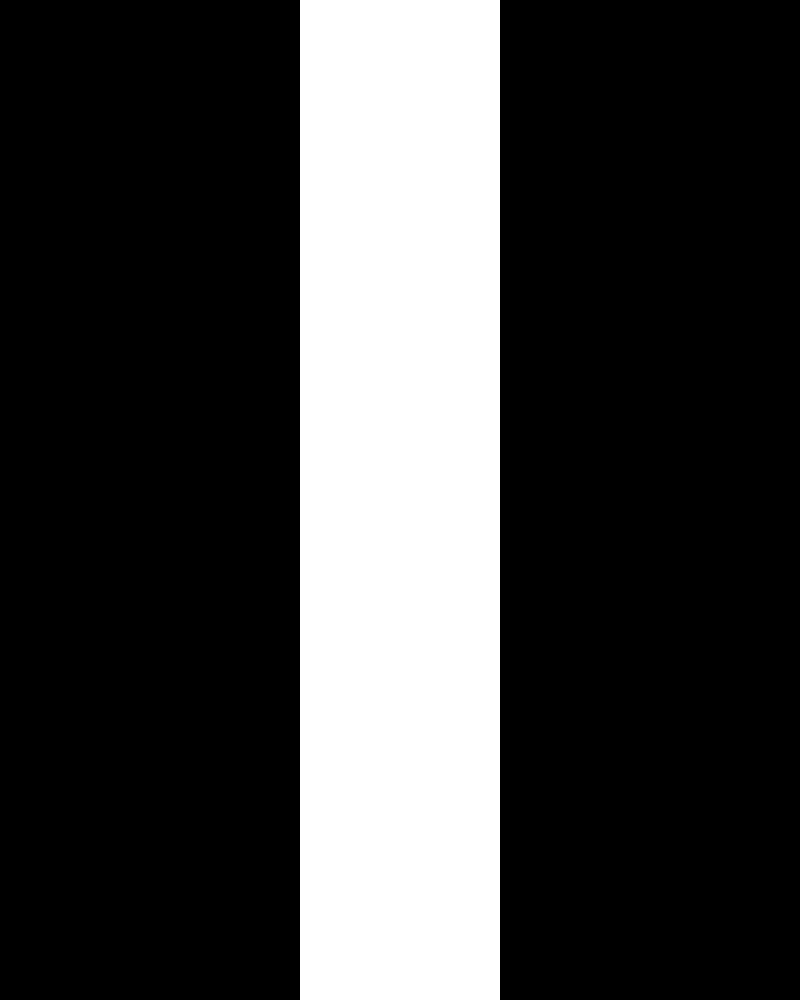
\includegraphics[width=.1\textwidth]{corogfx/icon_pause.png}};
  \end{tikzpicture}
  }
  \end{onlyenv}
  \begin{onlyenv}<5>
  \resizebox{.008\textwidth}{!}{%
  \begin{tikzpicture}[node distance = 0mm and 5mm,overlay]
    \node at([shift={(82ex,5ex)}]0,0) (main){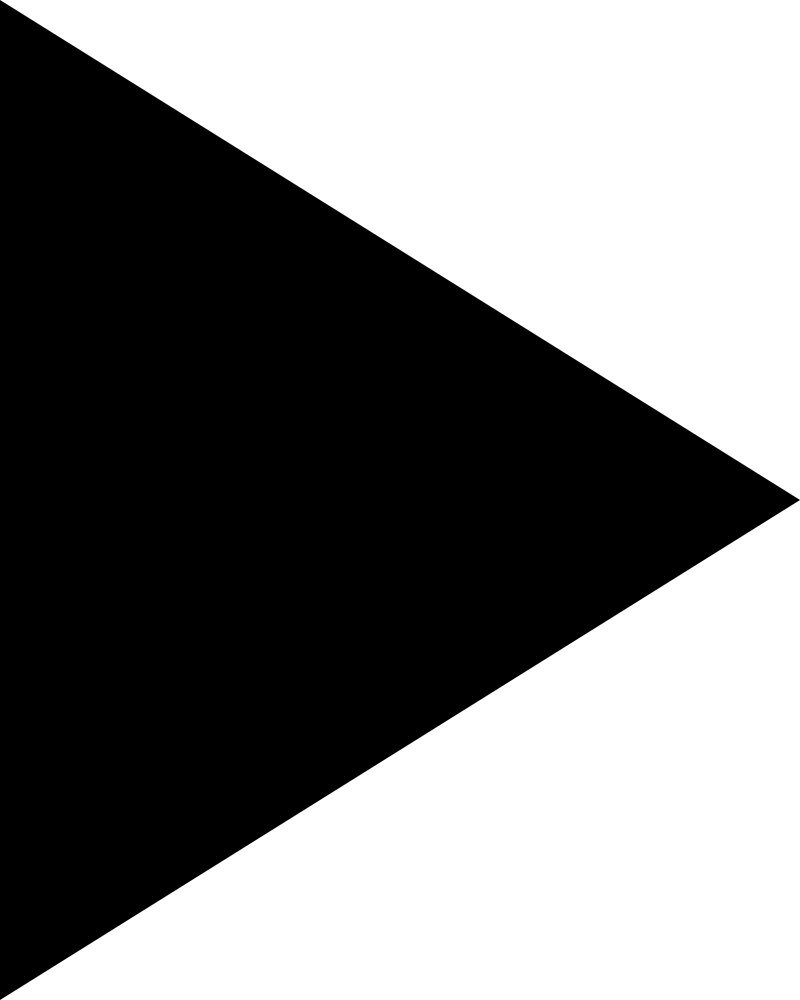
\includegraphics[width=.1\textwidth]{corogfx/icon_play.png}};
  \end{tikzpicture}
  }
  \end{onlyenv}
  \begin{onlyenv}<6>
  \resizebox{.008\textwidth}{!}{%
  \begin{tikzpicture}[node distance = 0mm and 5mm,overlay]
    \node at([shift={(82ex,5ex)}]0,0) (main) [stackframe]   {...};
    \node (outer)   [stackframe,above=of main]             {outer\_function()};
    \node (await)   [stackframe,above=of outer,style={fill=green!20}]            {Async<>::await\_resume};
  \end{tikzpicture}
  }
  \end{onlyenv}

  \begin{onlyenv}<9>
  \resizebox{.04\textwidth}{!}{%
  \begin{tikzpicture}[node distance = 0mm and 5mm,overlay]
    \node at([shift={(15ex,1.5ex)}]0,0) (main) {\Huge\Lightning};
  \end{tikzpicture}
  }
  \end{onlyenv}

  \note{
  \begin{itemize}
  \item \alert<+>{let's take a closer look; in outer func, we call middle}
  \item \alert<+>{***TRANSITION*** this returns us an awaitable}
  \item \alert<+>{***TRANSITION*** when awaiting it we call await\_suspend}
  \item \alert<+>{***TRANSITION*** and then outer is paused}
  \item \alert<+>{***TRANSITION*** when outer resumes}
  \item \alert<+>{***TRANSITION*** we end up in await\_resume}
  \item \alert<+>{***TRANSITION*** and then we step back in the function}
  \item ***TRANSITION*** BZZZZZT! We stepped too far.
  \end{itemize}
  }
\end{frame}

\begin{frame}
  Resuming nested suspended coroutines from the outside in does not work!

  \cpause
  \begin{itemize}
  \item Once a coroutine has been resumed, it cannot be suspended, unless we call \texttt{co\_await} again \cpause
  \item We do not know from the outside how often we need to resume an inner function before it succeeds \cpause
  \item We want \texttt{co\_await}ing an async function to mean: Wake me up once that function has completed and its result is available.
  \end{itemize}

\end{frame}


\begin{frame}
  \frametitle{Roadmap}
  \begin{todolist}
  \item Spawn outermost coroutine
  \only<1> {\item[\done] \textcolor{darkred}{Call nested coroutines}}
  \only<2> {\item[\wontfix] Call nested coroutines}
  \only<1> {\item[\done] \textcolor{darkred}{Suspend entire coroutine stack}}
  \only<2> {\item[\wontfix] Suspend entire coroutine stack}
  \item Resume entire coroutine stack
  \item Deliver final result
  \end{todolist}
\end{frame}


\begin{frame}
  \frametitle{What is a call stack anyway?}

  \cpause

   Anatomy of a stack frame
   \vspace{20pt}

   \begin{onlyenv}<2>
   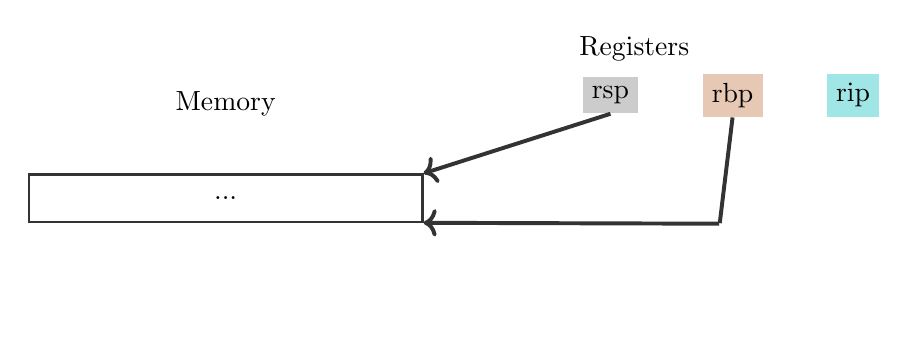
\begin{tikzpicture}[node distance = 0mm and 5mm,
    point/.style={circle,inner sep=0pt,minimum size=0pt,fill=black!100},
    memcell/.style={rectangle,minimum size=6mm,minimum width=50mm,thick,draw=black!80},
    invis/.style={rectangle,minimum size=6mm,minimum width=50mm,thick,draw=black!0},
   ]

    \node (func) [memcell]  { ... };
    \node (fp)   [invis,below=of func]  {}; \node (point_fp) [point,right=of fp,shift={(21.5ex,2ex)}]{};
    \node (ip)   [invis,below=of fp]  {};

    \node (rsp) [above right=of func,shift={(10ex,5ex)},fill=black!20] { rsp };
    \node (rbp) [right=of rsp,shift={(2ex,0ex)}, fill={rgb,255:red,230; green,200; blue,180}] { rbp };
    \node (rip) [right=of rbp,shift={(2ex,0ex)}, fill={rgb,255:red,160; green,230; blue,230}] { rip };

    \node (reg) [above=of rsp,shift={(2ex,0.5ex)}] { Registers };
    \node (mem) [above=of func,shift={(0,4ex)}] { Memory };

    \draw[line width=0.5mm, black!80] (rsp.south) edge[->] (func.north east);
    \draw[line width=0.5mm, black!80] (rbp.south) edge (point_fp)
          (point_fp) edge[->] (func.south east);
   \end{tikzpicture}
   \end{onlyenv}
   \begin{onlyenv}<3>
   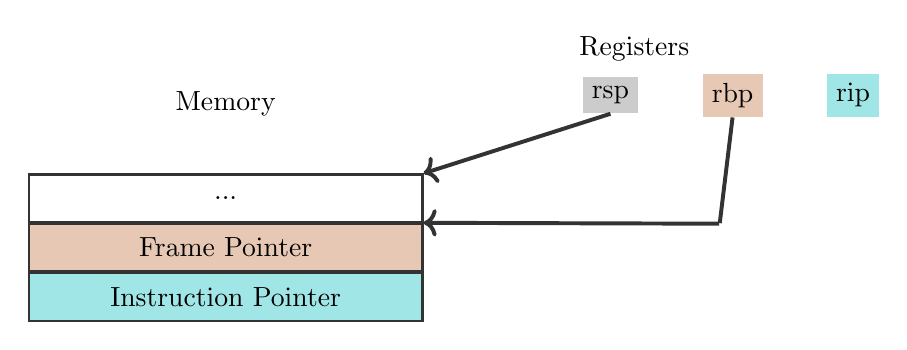
\begin{tikzpicture}[node distance = 0mm and 5mm,
    point/.style={circle,inner sep=0pt,minimum size=0pt,fill=black!100},
    memcell/.style={rectangle,minimum size=6mm,minimum width=50mm,thick,draw=black!80},
   ]

    \node (func) [memcell]  { ... };
    \node (fp)   [memcell,below=of func, fill={rgb,255:red,230; green,200; blue,180}]  { Frame Pointer }; \node (point_fp) [point,right=of fp,shift={(21.5ex,2ex)}]{};
    \node (ip)   [memcell,below=of fp, fill={rgb,255:red,160; green,230; blue,230}]  { Instruction Pointer };

    \node (rsp) [above right=of func,shift={(10ex,5ex)},fill=black!20] { rsp };
    \node (rbp) [right=of rsp,shift={(2ex,0ex)}, fill={rgb,255:red,230; green,200; blue,180}] { rbp };
    \node (rip) [right=of rbp,shift={(2ex,0ex)}, fill={rgb,255:red,160; green,230; blue,230}] { rip };

    \node (reg) [above=of rsp,shift={(2ex,0.5ex)}] { Registers };
    \node (mem) [above=of func,shift={(0,4ex)}] { Memory };

    \draw[line width=0.5mm, black!80] (rsp.south) edge[->] (func.north east);
    \draw[line width=0.5mm, black!80] (rbp.south) edge (point_fp)
          (point_fp) edge[->] (fp.north east);
   \end{tikzpicture}
   \end{onlyenv}

  \note{
    \color{green}{TIME!} \color{black}{0:20}
    \begin{itemize}
    \item what is a call stack anyway?
    \item ***TRANSITION*** function state between rsp and rbp
    \item ***TRANSITION*** below that fp and ip for our caller
    \end{itemize}
  }
\end{frame}

\begin{frame}
  \frametitle{What is a call stack anyway?}

  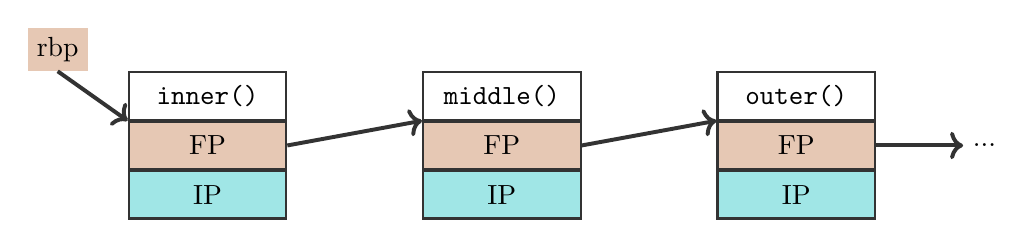
\begin{tikzpicture}[node distance = 0mm and 5mm,
    point/.style={circle,inner sep=0pt,minimum size=0pt,fill=black!100},
    memcell/.style={rectangle,minimum size=6mm,minimum width=20mm,thick,draw=black!80},
   ]

    \node (rbp) [fill={rgb,255:red,230; green,200; blue,180}] { rbp };

    \node (func1) [memcell,below right=of rbp,style={font=\ttfamily}]  { inner() };
    \node (fp1)   [memcell,below=of func1, fill={rgb,255:red,230; green,200; blue,180}]  { FP };
    \node (ip1)   [memcell,below=of fp1, fill={rgb,255:red,160; green,230; blue,230}]  { IP };

    \node (func2) [memcell,right=of func1,shift={(8ex,0)},style={font=\ttfamily}]  { middle() };
    \node (fp2)   [memcell,below=of func2, fill={rgb,255:red,230; green,200; blue,180}]  { FP };
    \node (ip2)   [memcell,below=of fp2, fill={rgb,255:red,160; green,230; blue,230}]  { IP };

    \node (func3) [memcell,right=of func2,shift={(8ex,0)},style={font=\ttfamily}]  { outer() };
    \node (fp3)   [memcell,below=of func3, fill={rgb,255:red,230; green,200; blue,180}]  { FP };
    \node (ip3)   [memcell,below=of fp3, fill={rgb,255:red,160; green,230; blue,230}]  { IP };

    \node (dotdot) [right=of fp3,shift={(4ex,0)}] {...};

    \draw[line width=0.5mm, black!80] (rbp.south) edge[->] (fp1.north west);
    \draw[line width=0.5mm, black!80] (fp1.east) edge[->] (fp2.north west);
    \draw[line width=0.5mm, black!80] (fp2.east) edge[->] (fp3.north west);
    \draw[line width=0.5mm, black!80] (fp3.east) edge[->] (dotdot.west);
  \end{tikzpicture}

  \vspace{3em}
  $\Rightarrow$ Singly-linked list of stack frames with links from callee-frame to caller-frame.

  \note{
  \begin{itemize}
  \item linked list
  \item how do we build something like this with coroutines?
  \end{itemize}
  }
\end{frame}

\begin{frame}
  \frametitle{Roadmap}
  \begin{todolist}
  \item Spawn outermost coroutine \cpause
  \only<1-8>{ \item \alert<8>{Call nested coroutines} } \cpause
  \only<9>{ \item \textcolor{darkred}{Call nested coroutines and establish links from callee to caller}}
  \item Suspend innermost coroutine \cpause
  \item Resume innermost coroutine \cpause
  \item Resume outer coroutine from inner coroutine \only<7>{\textcolor{darkred}{???}} \cpause
  \item Deliver final result
  \end{todolist}
\end{frame}

\begin{frame}[fragile]
  \frametitle{Connecting a coroutine to its caller}

  \begin{lstlisting}[style=cpp20]
(*@\danch(ar241)@*)Async<IoResult>(*@\danch(br241)@*) (*@\danch(ar245)@*)inner_function()(*@\danch(br245)@*) {
    // ...
}

Async<PartialResult> (*@\danch(ar246)@*)middle_function()(*@\danch(br246)@*) {
  (*@\danch(ar242)@*)Async<IoResult>(*@\danch(br242)@*) awaitable = inner_function();
  IoResult r = co_await awaitable();
  co_return PartialResult::from_io_result(r);
}
  \end{lstlisting}
  \monobox[indigo](ar245:br245)
  \monobox[orange](ar246:br246)
  \begin{onlyenv}<2>
  \monobox[blue](ar241:br241)
  \monobox[green](ar242:br242)
  \end{onlyenv}

  \note{
  \begin{itemize}
  \item inner=indigo, outer=orange
  \item ***TRANSITION*** same Async in two roles
  \end{itemize}
  }
\end{frame}

\iffalse
\begin{frame}[fragile]
  \frametitle{A look at the cheat sheet...}

  \begin{center}
  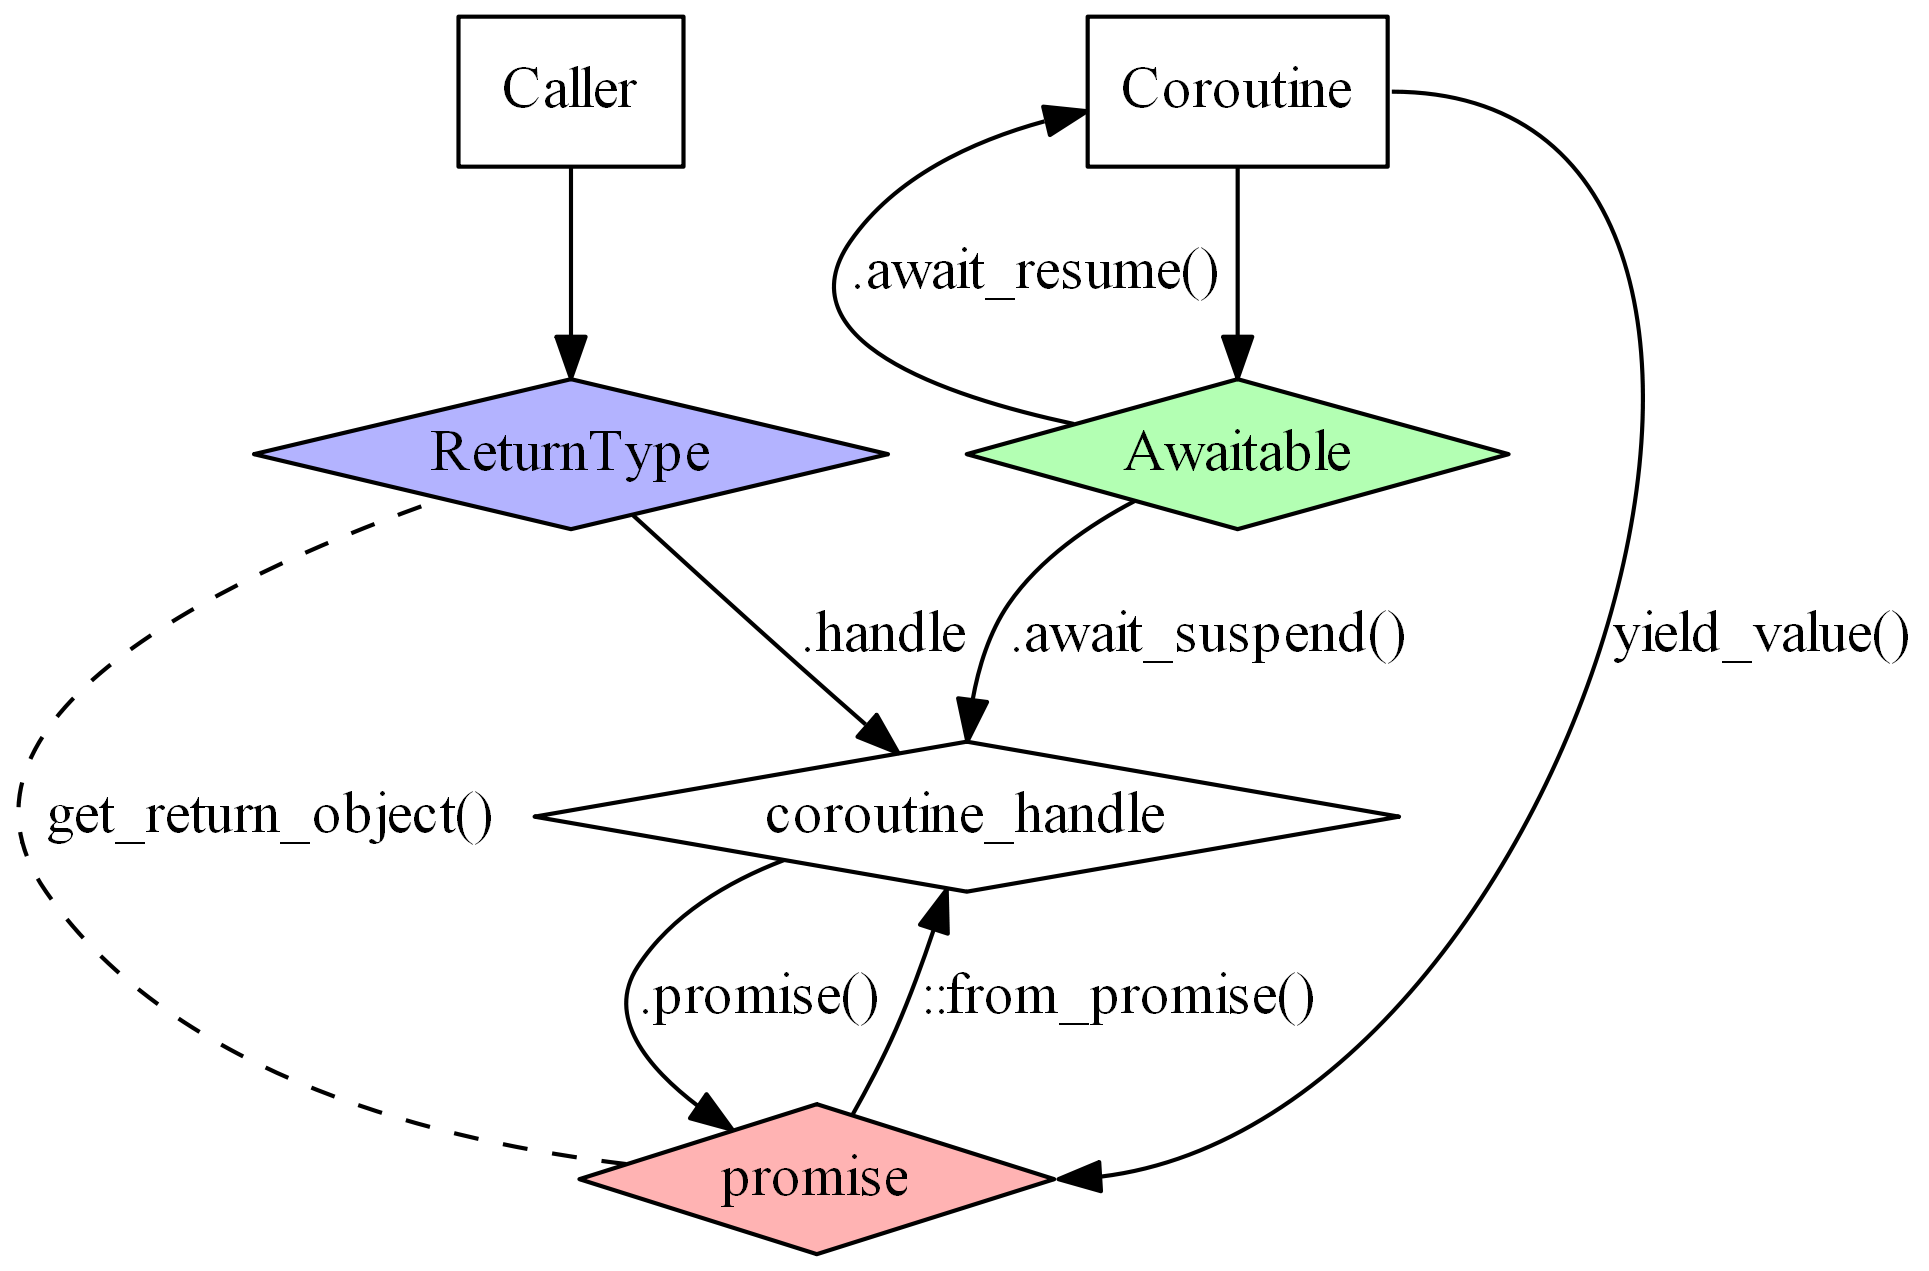
\includegraphics[height=.9\textheight]{corogfx/acquaintances05.png}
  \end{center}

  \note{
  \begin{itemize}
    \item The inner coroutine builds an Async object and hands it to the caller
    \item The caller then awaits that Async object to get notified when the inner coroutine finishes
    \item Note that in this diagram the caller and the coroutine are the same function for the same Async object!
    \item The inner coroutine does not have access to that Async object anymore! It can only reach it via the promise (by awaiting on a different awaitable than the one it returned)!
  \end{itemize}
  }
\end{frame}
\fi

\begin{frame}[fragile]
  \frametitle{Setting up the \texttt{Async} object}
  
  \iftransitions
  \begin{onlyenv}<1>
  \begin{lstlisting}[style=cpp20]
template<typename T> struct (*@\danch(ar251)@*)Async(*@\danch(br251)@*) {
  struct promise_type { /* ... */





  };




};

.
  \end{lstlisting}
  \monobox[blue](ar251:br251)
  \end{onlyenv}
  \begin{onlyenv}<2>
  \begin{lstlisting}[style=cpp20]
template<typename T> struct (*@\danch(ar251)@*)Async(*@\danch(br251)@*) {
  struct promise_type { /* ... */





  };
  (*@\danch(ar252)@*)std::coroutine_handle<promise_type> self(*@\danch(br252)@*);



};

.
  \end{lstlisting}
  \monobox[blue](ar251:br251)
  \monobox[indigo](ar252:br252)
  \end{onlyenv}
  \begin{onlyenv}<3>
    \begin{lstlisting}[style=cpp20]
template<typename T> struct (*@\danch(ar251)@*)Async(*@\danch(br251)@*) {
  struct promise_type { /* ... */
    (*@\danch(ar253)@*)Async<T>(*@\danch(br253)@*) get_return_object() {
      auto h = std::coroutine_handle<promise_type>
                ::from_promise(*this);
      return Async<T>{ h };
    }
  };
  (*@\danch(ar252)@*)std::coroutine_handle<promise_type> self(*@\danch(br252)@*);
  Async<T>((*@\danch(ar254)@*)std::coroutine_handle<promise_type> h(*@\danch(br254)@*))
    :self(h)
  {}
};

.
  \end{lstlisting}
  \monobox[blue](ar251:br251)
  \monobox[blue](ar253:br253)
  \monobox[indigo](ar252:br252)
  \monobox[indigo](ar254:br254)
  \end{onlyenv}
  \begin{onlyenv}<4>
    \begin{lstlisting}[style=cpp20]
template<typename T> struct (*@\danch(ar251)@*)Async(*@\danch(br251)@*) {
  struct promise_type { /* ... */ };


  (*@\danch(ar252)@*)std::coroutine_handle<promise_type> self(*@\danch(br252)@*);







};

.
  \end{lstlisting}
  \monobox[blue](ar251:br251)
  \monobox[indigo](ar252:br252)
  \end{onlyenv}


  \else
  \begin{lstlisting}[style=cpp20]
template<typename T> struct (*@\danch(ar251)@*)Async(*@\danch(br251)@*) {
  struct promise_type {
    /* ... */
    (*@\danch(ar253)@*)Async<T>(*@\danch(br253)@*) get_return_object() {
      auto h = std::coroutine_handle<promise_type>
                ::from_promise(*this);
      return Async<T>{ h };
    }
  };
  (*@\danch(ar252)@*)std::coroutine_handle<promise_type> self(*@\danch(br252)@*);
  Async<T>((*@\danch(ar254)@*)std::coroutine_handle<promise_type> h(*@\danch(br254)@*))
    :self(h)
  {}
};
.
  \end{lstlisting}
  \monobox[blue](ar251:br251)
  \monobox[blue](ar253:br253)
  \monobox[indigo](ar252:br252)
  \monobox[indigo](ar254:br254)
  \fi

  \note{
  \textit{Two roles separated; first return}
  \begin{itemize}
  \item \alert<+>{first the return object perspective}
  \item \alert<+>{***TRANSITION*** we add a handle to the inner coro}
  \item \alert<+>{***TRANSITION*** populating from get\_return\_object; standard stuff; handle is inner}
  \item ***TRANSITION*** that's all we can do for return obj
  \end{itemize}
  }
\end{frame}

\begin{frame}[fragile]
  \frametitle{Connecting a coroutine to its caller}

  \begin{onlyenv}<1>
   \begin{lstlisting}[style=cpp20]
template<typename T> struct (*@\danch(ar251)@*)Async(*@\danch(br251)@*) {
  struct promise_type { /* ... */ };


  (*@\danch(ar252)@*)std::coroutine_handle<promise_type> self(*@\danch(br252)@*);







};

.
  \end{lstlisting}
  \monobox[indigo](ar252:br252)
  \monobox[green](ar251:br251)
  \end{onlyenv}
  \begin{onlyenv}<2>
   \begin{lstlisting}[style=cpp20]
template<typename T> struct (*@\danch(ar251)@*)Async(*@\danch(br251)@*) {
  struct promise_type { /* ... */ };


  (*@\danch(ar252)@*)std::coroutine_handle<promise_type> self(*@\danch(br252)@*);


  bool await_ready() { return false; }
  T await_resume() { /* ... */ }
  auto await_suspend((*@\danch(ar254)@*)std::coroutine_handle<> handle(*@\danch(br254)@*)) {

  }
};

.
  \end{lstlisting}
  \monobox[indigo](ar252:br252)
  \monobox[green](ar251:br251)
  \end{onlyenv}
  \begin{onlyenv}<3>
   \begin{lstlisting}[style=cpp20]
template<typename T> struct (*@\danch(ar251)@*)Async(*@\danch(br251)@*) {
  struct promise_type { /* ... */ };


  (*@\danch(ar252)@*)std::coroutine_handle<promise_type> self(*@\danch(br252)@*);


  bool await_ready() { return false; }
  T await_resume() { /* ... */ }
  auto await_suspend((*@\danch(ar254)@*)std::coroutine_handle<> handle(*@\danch(br254)@*)) {

  }
};

.
  \end{lstlisting}
  \monobox[indigo](ar252:br252)
  \monobox[orange](ar254:br254)
  \monobox[green](ar251:br251)
  \end{onlyenv}

  \begin{onlyenv}<4>
   \begin{lstlisting}[style=cpp20]
template<typename T> struct (*@\danch(ar251)@*)Async(*@\danch(br251)@*) {
  struct promise_type { /* ... */ 
    (*@\danch(ar253)@*)std::coroutine_handle<> my_caller(*@\danch(br253)@*);
  };
  (*@\danch(ar252)@*)std::coroutine_handle<promise_type> self(*@\danch(br252)@*);


  bool await_ready() { return false; }
  T await_resume() { /* ... */ }
  auto await_suspend((*@\danch(ar254)@*)std::coroutine_handle<> handle(*@\danch(br254)@*)) {
    self.promise().my_caller = handle;
  }
};

.
  \end{lstlisting}
  \monobox[indigo](ar252:br252)
  \monobox[orange](ar253:br253)
  \monobox[orange](ar254:br254)
  \monobox[green](ar251:br251)
  \end{onlyenv}

  \note{
  \begin{itemize}
  \item \alert<+>{switch to awaitable; this is the role in the outer function}
  \item \alert<+>{***TRANSITION*** we need the three funcs; note the handle in suspend}
  \item \alert<+>{***TRANSITION*** it's handle to outer; make sure people understand why}
  \item ***TRANSITION*** save outer handle
  \end{itemize}
  }
\end{frame}


\begin{frame}
  \frametitle{We have our own call stack now}

  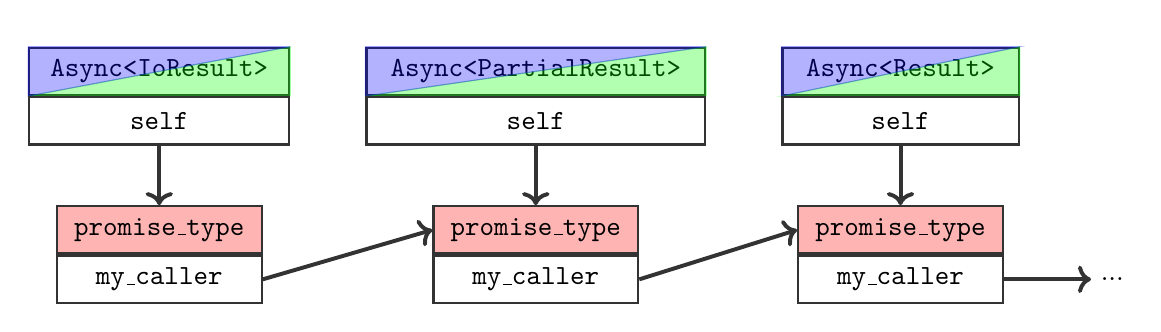
\begin{tikzpicture}[node distance = 0mm and 5mm,
    point/.style={circle,inner sep=0pt,minimum size=0pt,fill=black!100},
    memcell/.style={rectangle,minimum size=6mm,minimum width=26mm,thick,draw=black!80,font=\ttfamily},
   ]

    \node (rbp) {};

    \node (func1) [memcell,below=of rbp,style={minimum width=33mm}]  { Async<IoResult> };
    \filldraw[green, opacity=0.3][] (func1.south west)
        -- (func1.south east)
        -- (func1.north east)--cycle
        ;
    \filldraw[blue, opacity=0.3][] (func1.south west)
        -- (func1.north west)
        -- (func1.north east)--cycle
        ;
    \node (self1)   [memcell,below=of func1,style={minimum width=33mm}]  { self };
    \node (promise1)   [memcell,below=of self1,shift={(0ex,-5ex)}, fill={rgb,255:red,255; green,180; blue,180}]  { promise\_type };
    \node (caller1)   [memcell,below=of promise1]  { my\_caller };

    \node (func2) [memcell,right=of func1,shift={(3ex,0)},style={minimum width=43mm}]  { Async<PartialResult> };
    \filldraw[green, opacity=0.3][] (func2.south west)
        -- (func2.south east)
        -- (func2.north east)--cycle
        ;
    \filldraw[blue, opacity=0.3][] (func2.south west)
        -- (func2.north west)
        -- (func2.north east)--cycle
        ;
    \node (self2)   [memcell,below=of func2,,style={minimum width=43mm}]  { self };
    \node (promise2)   [memcell,below=of self2,shift={(0ex,-5ex)}, fill={rgb,255:red,255; green,180; blue,180}]  { promise\_type };
    \node (caller2)   [memcell,below=of promise2]  { my\_caller };

    \node (func3) [memcell,right=of func2,shift={(3ex,0)},style={minimum width=30mm}]  { Async<Result> };
    \filldraw[green, opacity=0.3][] (func3.south west)
        -- (func3.south east)
        -- (func3.north east)--cycle
        ;
    \filldraw[blue, opacity=0.3][] (func3.south west)
        -- (func3.north west)
        -- (func3.north east)--cycle
        ;
    \node (self3)   [memcell,below=of func3,style={minimum width=30mm}]  { self };
    \node (promise3)   [memcell,below=of self3,shift={(0ex,-5ex)}, fill={rgb,255:red,255; green,180; blue,180}]  { promise\_type };
    \node (caller3)   [memcell,below=of promise3]  { my\_caller };

    \node (dotdot) [right=of caller3,shift={(4ex,0)}] {...};

    \draw[line width=0.5mm, black!80] (self1.south) edge[->] (promise1.north);
    \draw[line width=0.5mm, black!80] (self2.south) edge[->] (promise2.north);
    \draw[line width=0.5mm, black!80] (self3.south) edge[->] (promise3.north);
    \draw[line width=0.5mm, black!80] (caller1.east) edge[->] (promise2.west);
    \draw[line width=0.5mm, black!80] (caller2.east) edge[->] (promise3.west);
    \draw[line width=0.5mm, black!80] (caller3.east) edge[->] (dotdot.west);
  \end{tikzpicture}

  \note{ \color{green}{TIME!} \color{black}{0:25} }
\end{frame}


\begin{frame}
  \frametitle{Roadmap}
  \begin{todolist}
  \item Spawn outermost coroutine
  \only<1>{ \item \textcolor{darkred}{Call nested coroutines and establish links from callee to caller}}
  \only<2->{ \item[\done] Call nested coroutines and establish links from callee to caller}
  \item Suspend innermost coroutine
  \item Resume innermost coroutine
  \item \alert<3>{Resume outer coroutine from inner coroutine}
  \item Deliver final result
  \end{todolist}
\end{frame}


\begin{frame}[fragile]
  \frametitle{Resuming the caller from a nested coroutine}

  \begin{onlyenv}<2>
  \begin{lstlisting}[style=cpp20]
template<typename T>
struct (*@\danch(ar271)@*)Async(*@\danch(br271)@*) {
  struct promise_type { /* ... */ 
    (*@\danch(ar272)@*)std::coroutine_handle<> my_caller(*@\danch(br272)@*);



  };
};





.
  \end{lstlisting}
  \monobox[blue](ar271:br271)
  \monobox[orange](ar272:br272)
  \end{onlyenv}
  \begin{onlyenv}<3>
  \begin{lstlisting}[style=cpp20]
template<typename T>
struct (*@\danch(ar271)@*)Async(*@\danch(br271)@*) {
  struct promise_type { /* ... */ 
    (*@\danch(ar272)@*)std::coroutine_handle<> my_caller(*@\danch(br272)@*);
    auto final_suspend() noexcept {
      return ResumeCaller{};
    }
  };
};

struct (*@\danch(ar274)@*)ResumeCaller(*@\danch(br274)@*);



.
  \end{lstlisting}
  \monobox[blue](ar271:br271)
  \monobox[green](ar274:br274)
  \monobox[orange](ar272:br272)
  \end{onlyenv}
  \begin{onlyenv}<4>
  \begin{lstlisting}[style=cpp20]
struct promise_type { /* ... */
  (*@\danch(ar277)@*)std::coroutine_handle<> my_caller(*@\danch(br277)@*);
};
struct (*@\danch(ar274)@*)ResumeCaller(*@\danch(br274)@*) {








};

.
  \end{lstlisting}
  \monobox[green](ar274:br274)
  \monobox[orange](ar277:br277)
  \end{onlyenv}
  \begin{onlyenv}<5>
  \begin{lstlisting}[style=cpp20]
struct promise_type { /* ... */
  (*@\danch(ar277)@*)std::coroutine_handle<> my_caller(*@\danch(br277)@*);
};
struct (*@\danch(ar274)@*)ResumeCaller(*@\danch(br274)@*) {
  bool await_ready() { return false; }
  void await_resume() { /* will never be called! */ }






};

.
  \end{lstlisting}
  \monobox[green](ar274:br274)
  \monobox[orange](ar277:br277)
  \end{onlyenv}
  \begin{onlyenv}<6>
  \begin{lstlisting}[style=cpp20]
struct promise_type { /* ... */
  (*@\danch(ar277)@*)std::coroutine_handle<> my_caller(*@\danch(br277)@*);
};
struct (*@\danch(ar274)@*)ResumeCaller(*@\danch(br274)@*) {
  bool await_ready() { return false; }
  void await_resume() { /* will never be called! */ }

  (*@\danch(ar275)@*)coroutine_handle<>(*@\danch(br275)@*) await_suspend(
      coroutine_handle<promise_type> h) {

    return h.promise().(*@\danch(ar276)@*)my_caller(*@\danch(br276)@*);
  }
};

.
  \end{lstlisting}
  \monobox[green](ar274:br274)
  \monobox[orange](ar275:br275)
  \monobox[orange](ar276:br276)
  \monobox[orange](ar277:br277)
  \end{onlyenv}
  \begin{onlyenv}<7>
  \begin{lstlisting}[style=cpp20]
struct promise_type { /* ... */
  (*@\danch(ar277)@*)std::coroutine_handle<> my_caller(*@\danch(br277)@*);
};
struct (*@\danch(ar274)@*)ResumeCaller(*@\danch(br274)@*) {
  bool await_ready() { return false; }
  void await_resume() { /* will never be called! */ }

  (*@\danch(ar275)@*)coroutine_handle<>(*@\danch(br275)@*) await_suspend(
      coroutine_handle<promise_type> h) {
    // (*@\color{red}{\textit{Symmetric Transfer!}}@*)
    return h.promise().(*@\danch(ar276)@*)my_caller(*@\danch(br276)@*);
  }
};

.
  \end{lstlisting}
  \monobox[green](ar274:br274)
  \monobox[orange](ar275:br275)
  \monobox[orange](ar276:br276)
  \monobox[orange](ar277:br277)
  \end{onlyenv}

  \note{
  \begin{itemize}
  \item \alert<+>{we have the links, now we can resume from inside out}
  \item \alert<+>{***TRANSITION*** we have handle to outer in promise; when do we want to use this?}
  \item \alert<+>{***TRANSITION*** in final\_suspend we await on outer}
  \item \alert<+>{***TRANSITION*** what does ResumeCaller look like?}
  \item \alert<+>{***TRANSITION*** await\_ready and await\_resume}
  \item \alert<+>{***TRANSITION*** await\_suspend returns handle}
  \item ***TRANSITION*** symmetric transfer!
  \end{itemize}
  }
\end{frame}

% \fi % !!!!!!!!!!!!!!

\begin{frame}[fragile]

  \frametitle{Resuming caller via symmetric transfer}
  \begin{lstlisting}[style=cpp20]
(*@\danch(ar310)@*)Async<> (*@\danch(ar311)@*)middle_function()(*@\danch(br311)@*) {
(*@\danch(ar320)@*)  auto r = co_await inner_function();
(*@\danch(ar330)@*)  co_return PartialResult::from_io_result(r);
(*@\danch(ar340)@*)}
(*@\danch(ar350)@*)Async<> (*@\danch(ar351)@*)inner_function()(*@\danch(br351)@*) { /* ... */
(*@\danch(ar360)@*)  co_return IoResult::from_io_data(data);
(*@\danch(ar370)@*)}
  \end{lstlisting}
  \begin{onlyenv}<1-2>
  \begin{lstlisting}[style=cpp20]
  
  
  
  
  
  
  
  
  
  .
  \end{lstlisting}
  \end{onlyenv}
  \begin{onlyenv}<3>
  \begin{lstlisting}[style=cpp20]
(*@\danch(ar380)@*)auto (*@\danch(ar381)@*)promise_type(*@\danch(br381)@*)::final_suspend() {
(*@\danch(ar390)@*)  return ResumeCaller{};
(*@\danch(ar400)@*)}
  \end{lstlisting}
  \end{onlyenv}
  \begin{onlyenv}<4->
  \begin{lstlisting}[style=cpp20]
(*@\danch(ar410)@*)auto (*@\danch(ar411)@*)ResumeCaller(*@\danch(br411)@*)::await_suspend(
    coroutine_handle<promise_type> h) {
(*@\danch(ar420)@*)  return h.promise().my_caller;
(*@\danch(ar430)@*)}
  \end{lstlisting}
  \end{onlyenv}

  \monobox[orange](ar311:br311)
  \monobox[indigo](ar351:br351)
  \only<3>{ \monobox[red](ar381:br381) }
  \only<4->{ \monobox[green](ar411:br411) }

  \only<1-5>{\tikz[transform shape,overlay] \draw[>=triangle 45,->,teal,very thick] ([shift={(-1em,0.25em)}]ar320.north) -- ([shift={(1em,0.25em)}]ar320.north);}
  \only<6-7>{\tikz[transform shape,overlay] \draw[>=triangle 45,->,darkred,very thick] ([shift={(-1em,0.25em)}]ar320.north) -- ([shift={(1em,0.25em)}]ar320.north);}
  \only<8>{\tikz[transform shape,overlay] \draw[>=triangle 45,->,darkred,very thick] ([shift={(-1em,0.25em)}]ar330.north) -- ([shift={(1em,0.25em)}]ar330.north);}
  \only<1-2>{\tikz[transform shape,overlay] \draw[>=triangle 45,->,darkred,very thick] ([shift={(-1em,0.25em)}]ar360.north) -- ([shift={(1em,0.25em)}]ar360.north);}
  \only<3>{\tikz[transform shape,overlay] \draw[>=triangle 45,->,darkred,very thick] ([shift={(-1em,0.25em)}]ar390.north) -- ([shift={(1em,0.25em)}]ar390.north);}
  \only<4>{\tikz[transform shape,overlay] \draw[>=triangle 45,->,darkred,very thick] ([shift={(-1em,0.25em)}]ar420.north) -- ([shift={(1em,0.25em)}]ar420.north);}
  \only<5>{\tikz[transform shape,overlay] \draw[>=triangle 45,->,darkred,very thick] ([shift={(-1em,0.25em)}]ar430.north) -- ([shift={(0.2em,0.25em)}]ar430.north);}

  \begin{onlyenv}<1>
  \scalebox{0.7}{
  \begin{tikzpicture}[node distance = 0mm and 5mm,overlay]
    \node (main) at ([shift={(17cm,-0.5cm)}]ar350.east) [stackframe,fill=lightgray,style={minimum width=80mm}] {base()};
    \node (inner)   [stackframe,fill=indigo!30,above=of main,style={minimum width=80mm}]  {inner\_function()};
    \node (await)   [above=of inner,style={minimum size=6mm,minimum width=80mm}]   {};
  \end{tikzpicture}
  }
  \end{onlyenv}
  \begin{onlyenv}<2>
  \scalebox{0.7}{
  \begin{tikzpicture}[node distance = 0mm and 5mm,overlay]
    \node (main) at ([shift={(17cm,-0.5cm)}]ar350.east) [stackframe,fill=lightgray,style={minimum width=80mm}] {base()};
    \node (inner)   [stackframe,fill=indigo!30,above=of main,style={minimum width=80mm}]  {inner\_function()};
    \node (retval)  [stackframe,fill=co_promise,above=of inner,style={minimum width=80mm}] {promise\_type::return\_value()};
  \end{tikzpicture}
  }
  \end{onlyenv}
  \begin{onlyenv}<3>
  \scalebox{0.7}{
  \begin{tikzpicture}[node distance = 0mm and 5mm,overlay]
    \node (main) at ([shift={(17cm,-1.9cm)}]ar350.east) [stackframe,fill=lightgray,style={minimum width=80mm}] {base()};
    \node (inner)   [stackframe,fill=indigo!30,above=of main,style={minimum width=80mm}]      {inner\_function()};
    \node (await)   [stackframe,above=of inner,fill=co_promise,style={minimum width=80mm}]   {Async<>::promise\_type::final\_suspend()};
  \end{tikzpicture}
  }
  \end{onlyenv}
  \begin{onlyenv}<4>
  \scalebox{0.7}{
  \begin{tikzpicture}[node distance = 0mm and 5mm,overlay]
    \node (main) at ([shift={(17cm,-1.5cm)}]ar350.east) [stackframe,fill=lightgray,style={minimum width=80mm}] {base()};
    \node (inner)   [stackframe,fill=indigo!30,above=of main,style={minimum width=80mm}]      {inner\_function()};
    \node (await)   [stackframe,above=of inner,fill=co_awaitable,style={minimum width=80mm}]   {ResumeCaller::await\_suspend()};
  \end{tikzpicture}
  }
  \end{onlyenv}
  \begin{onlyenv}<5>
  \scalebox{0.7}{
  \begin{tikzpicture}[node distance = 0mm and 5mm,overlay]
    \node (main) at ([shift={(17cm,-1.5cm)}]ar350.east) [stackframe,fill=lightgray,style={minimum width=80mm}] {base()};
    \node (inner)   [stackframe,fill=orange!30,above=of main,style={minimum width=80mm}]      {middle\_function()};
    \node (await)   [above=of inner,style={minimum size=6mm,minimum width=80mm}]   {};
  \end{tikzpicture}
  }
  \end{onlyenv}
  \begin{onlyenv}<6>
  \scalebox{0.7}{
  \begin{tikzpicture}[node distance = 0mm and 5mm,overlay]
    \node (main) at ([shift={(17cm,-1.5cm)}]ar350.east) [stackframe,fill=lightgray,style={minimum width=80mm}] {base()};
    \node (inner)   [stackframe,fill=orange!30,above=of main,style={minimum width=80mm}]      {middle\_function()};
    \node (await)   [stackframe,above=of inner,fill=co_awaitable,style={minimum width=80mm}]   {Async::await\_resume()};
  \end{tikzpicture}
  }
  \end{onlyenv}
  \begin{onlyenv}<7>
  \scalebox{0.7}{
  \begin{tikzpicture}[node distance = 0mm and 5mm,overlay]
    \node (main) at ([shift={(17cm,-1.5cm)}]ar350.east) [stackframe,fill=lightgray,style={minimum width=80mm}] {base()};
    \node (inner)   [stackframe,fill=orange!30,above=of main,style={minimum width=80mm}]      {middle\_function()};
    \node (await)   [above=of inner,style={minimum size=6mm,minimum width=80mm}]   {};
  \end{tikzpicture}
  }
  \end{onlyenv}
  \begin{onlyenv}<8>
  \scalebox{0.7}{
  \begin{tikzpicture}[node distance = 0mm and 5mm,overlay]
    \node (main) at ([shift={(17cm,-1.5cm)}]ar350.east) [stackframe,fill=lightgray,style={minimum width=80mm}] {base()};
    \node (inner)   [stackframe,fill=orange!30,above=of main,style={minimum width=80mm}]      {middle\_function()};
    \node (await)   [stackframe,fill=indigo!30,above=of inner,style={minimum width=80mm}]   {\~{}Async<IoResult>};
  \end{tikzpicture}
  }
  \end{onlyenv}
  
  \begin{onlyenv}<5-7>
  \begin{tikzpicture}[node distance = 0mm and 5mm,overlay]
    \node at([shift={(65ex,5cm)}]0,0) (main){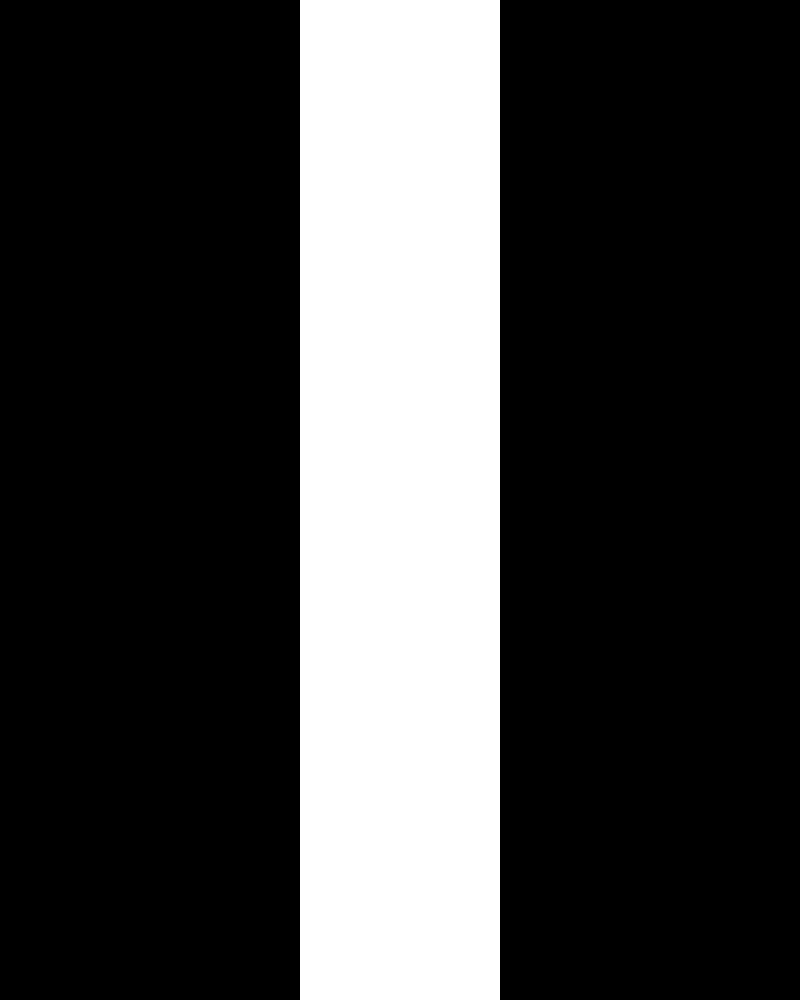
\includegraphics[width=.07\textwidth]{corogfx/icon_pause.png}};
  \end{tikzpicture}
  \end{onlyenv}

  \note{
  \begin{itemize}
  \item \alert<+>{call stack for resuming with symmetric transfer; base is frozen; inner above; goal is teal arrow}
  \item \alert<+>{***TRANSITION*** inner is done; store return\_value in promise}
  \item \alert<+>{***TRANSITION*** final suspend; triggers ResumeCaller via co\_await}
  \item \alert<+>{***TRANSITION*** ResumeCaller is awaited; returns handle to caller}
  \item \alert<+>{***TRANSITION*** symmetric transfer to middle; inner is suspended but still alive at this point}
  \item \alert<+>{***TRANSITION*** middle resumes; retrieves return value from inner promise}
  \item \alert<+>{***TRANSITION*** middle is moving on}
  \item ***TRANSITION*** inner Async goes out of scope; now inner is destroyed via Async's coroutine handle
  \end{itemize}
  }
\end{frame}

\begin{frame}[fragile]
  \frametitle{Resuming the caller from a nested coroutine}

  \begin{lstlisting}[style=cpp20]
template<typename T> struct (*@\danch(ar271)@*)Async(*@\danch(br271)@*) {
  struct promise_type { /* ... */ 
    (*@\danch(ar272)@*)coroutine_handle<> my_caller(*@\danch(br272)@*);
    auto final_suspend() noexcept {
      return ResumeCaller{};
    }
  };
};
struct (*@\danch(ar274)@*)ResumeCaller(*@\danch(br274)@*) { /* ... */
  auto await_suspend((*@\danch(ar277)@*)coroutine_handle<promise_type> h(*@\danch(br277)@*)) {
    return h.promise().(*@\danch(ar276)@*)my_caller(*@\danch(br276)@*);
  }
};
  \end{lstlisting}
  \monobox[blue](ar271:br271)
  \monobox[green](ar274:br274)
  \monobox[orange](ar272:br272)
  \monobox[orange](ar276:br276)
  \monobox[indigo](ar277:br277)
  
  \note{
  Overview slide
  }
\end{frame}


\begin{frame}
  \frametitle{Resuming caller via symmetric transfer}

  \begin{onlyenv}<1>
  \begin{center}
  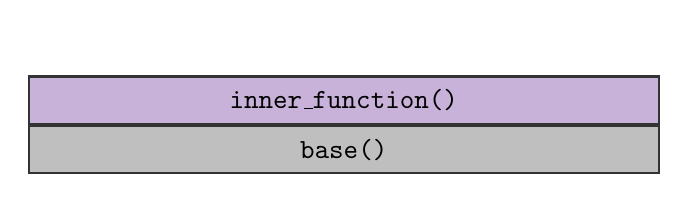
\begin{tikzpicture}[node distance = 0mm and 5mm]
    \node (main)    [stackframe,fill=lightgray,style={minimum width=80mm}] {base()};
    \node (inner)   [stackframe,fill=indigo!30,above=of main,style={minimum width=80mm}]  {inner\_function()};
    \node (await)   [above=of inner,style={minimum size=6mm,minimum width=80mm}]   {};
  \end{tikzpicture}
  \end{center}
  \end{onlyenv}
  \begin{onlyenv}<2>
  \begin{center}
  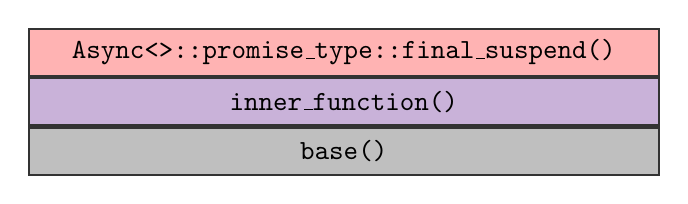
\begin{tikzpicture}[node distance = 0mm and 5mm]
    \node (main)    [stackframe,fill=lightgray,style={minimum width=80mm}]     {base()};
    \node (inner)   [stackframe,fill=indigo!30,above=of main,style={minimum width=80mm}]      {inner\_function()};
    \node (await)   [stackframe,above=of inner,fill=co_promise,style={minimum width=80mm}]   {Async<>::promise\_type::final\_suspend()};
  \end{tikzpicture}
  \end{center}
  \end{onlyenv}
  \begin{onlyenv}<3>
  \begin{center}
  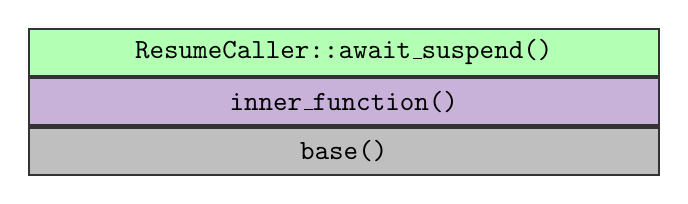
\begin{tikzpicture}[node distance = 0mm and 5mm]
    \node (main)    [stackframe,fill=lightgray,style={minimum width=80mm}]     {base()};
    \node (inner)   [stackframe,fill=indigo!30,above=of main,style={minimum width=80mm}]      {inner\_function()};
    \node (await)   [stackframe,above=of inner,fill=co_awaitable,style={minimum width=80mm}]   {ResumeCaller::await\_suspend()};
  \end{tikzpicture}
  \end{center}
  \end{onlyenv}
  \begin{onlyenv}<4>
  \begin{center}
  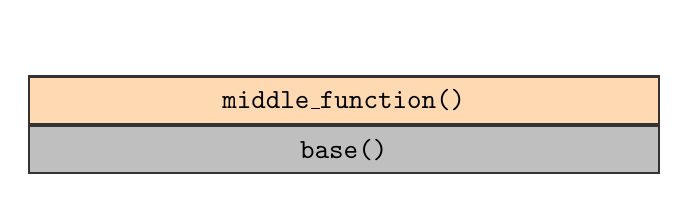
\begin{tikzpicture}[node distance = 0mm and 5mm]
    \node (main)    [stackframe,fill=lightgray,style={minimum width=80mm}]     {base()};
    \node (inner)   [stackframe,fill=orange!30,above=of main,style={minimum width=80mm}]      {middle\_function()};
    \node (await)   [above=of inner,style={minimum size=6mm,minimum width=80mm}]   {};
  \end{tikzpicture}
  \end{center}
  \end{onlyenv}
  \begin{onlyenv}<5->
  \begin{center}
  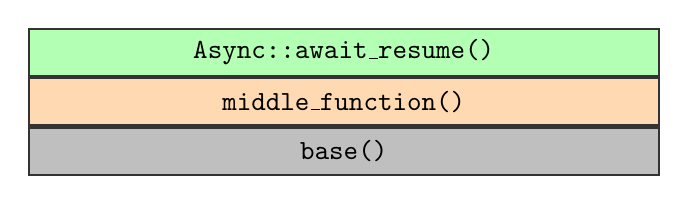
\begin{tikzpicture}[node distance = 0mm and 5mm]
    \node (main)    [stackframe,fill=lightgray,style={minimum width=80mm}]     {base()};
    \node (inner)   [stackframe,fill=orange!30,above=of main,style={minimum width=80mm}]      {middle\_function()};
    \node (await)   [stackframe,above=of inner,fill=co_awaitable,style={minimum width=80mm}]   {Async::await\_resume()};
  \end{tikzpicture}
  \end{center}
  \end{onlyenv}

  \note{
  \begin{itemize}
  \item \alert<+>{call stack for resuming with symmetric transfer; base is frozen; inner above;}
  \item \alert<+>{***TRANSITION*** inner is done; final suspend; triggers ResumeCaller}
  \item \alert<+>{***TRANSITION*** ResumeCaller is awaited}
  \item \alert<+>{***TRANSITION*** symmetric transfer to middle}
  \item ***TRANSITION*** middle resumes
  \end{itemize}
  }
\end{frame}

\begin{frame}
  \frametitle{Roadmap}
  \begin{todolist}
  \item Spawn outermost coroutine
  \item[\done] Call nested coroutines and establish links from callee to caller
  \item Suspend innermost coroutine
  \item \alert<3>{Resume innermost coroutine}
  \only<1>{ \item \textcolor{darkred}{Resume outer coroutine from inner coroutine}}
  \only<2->{ \item[\done] Resume outer coroutine from inner coroutine}
  \item Deliver final result
  \end{todolist}
\end{frame}


\begin{frame}[fragile]
  \frametitle{Resuming the innermost coroutine}

  \begin{tikzpicture}[node distance = 0mm and 5mm,
    point/.style={circle,inner sep=0pt,minimum size=0pt,fill=black!100},
    memcell/.style={rectangle,minimum size=6mm,minimum width=26mm,thick,draw=black!80,font=\ttfamily},
   ]

    \node (rbp) {};

    \node (func1) [memcell,below=of rbp,style={minimum width=33mm}]  { Async<IoResult> };
    \filldraw[green, opacity=0.3][] (func1.south west)
        -- (func1.south east)
        -- (func1.north east)--cycle
        ;
    \filldraw[blue, opacity=0.3][] (func1.south west)
        -- (func1.north west)
        -- (func1.north east)--cycle
        ;
    \node (self1)   [memcell,below=of func1,style={minimum width=33mm}]  { self };
    \node (promise1)   [memcell,below=of self1,shift={(0ex,-5ex)}, fill={rgb,255:red,255; green,180; blue,180}]  { promise\_type };
    \node (caller1)   [memcell,below=of promise1]  { my\_caller };

    \node (func2) [memcell,right=of func1,shift={(1ex,0)},style={minimum width=43mm}]  { Async<PartialResult> };
    \filldraw[green, opacity=0.3][] (func2.south west)
        -- (func2.south east)
        -- (func2.north east)--cycle
        ;
    \filldraw[blue, opacity=0.3][] (func2.south west)
        -- (func2.north west)
        -- (func2.north east)--cycle
        ;
    \node (self2)   [memcell,below=of func2,,style={minimum width=43mm}]  { self };
    \node (promise2)   [memcell,below=of self2,shift={(0ex,-5ex)}, fill={rgb,255:red,255; green,180; blue,180}]  { promise\_type };
    \node (caller2)   [memcell,below=of promise2]  { my\_caller };

    \node (func3) [memcell,right=of func2,shift={(1ex,0)},style={minimum width=30mm}]  { Async<Result> };
    \filldraw[green, opacity=0.3][] (func3.south west)
        -- (func3.south east)
        -- (func3.north east)--cycle
        ;
    \filldraw[blue, opacity=0.3][] (func3.south west)
        -- (func3.north west)
        -- (func3.north east)--cycle
        ;
    \node (self3)   [memcell,below=of func3,style={minimum width=30mm}]  { self };
    \node (promise3)   [memcell,below=of self3,shift={(0ex,-5ex)}, fill={rgb,255:red,255; green,180; blue,180}]  { promise\_type };
    \node (caller3)   [memcell,below=of promise3]  { my\_caller };

    \node (dotdot) [right=of caller3,shift={(2ex,0)}] {...};

    \draw[line width=0.5mm, black!80] (self1.south) edge[->] (promise1.north);
    \draw[line width=0.5mm, black!80] (self2.south) edge[->] (promise2.north);
    \draw[line width=0.5mm, black!80] (self3.south) edge[->] (promise3.north);
    \draw[line width=0.5mm, black!80] (caller1.east) edge[->] (promise2.west);
    \draw[line width=0.5mm, black!80] (caller2.east) edge[->] (promise3.west);
    \draw[line width=0.5mm, black!80] (caller3.east) edge[->] (dotdot.west);
    \only<1>{\node (quest)  [left=of self1,shift={(0ex,4.5ex)},text=white] {???};}
    \only<2>{\node (quest)  [left=of self1,shift={(0ex,4.5ex)}] {???};}
    \only<2>{\draw[line width=0.5mm, black!80] (quest.south) edge[->] (self1.west);}
  \end{tikzpicture}

  \note{
  \color{green}{TIME!} \color{black}{0:30}
  \begin{itemize}
  \item \alert<+>{we have the chain}
  \item ***TRANSITION*** but who resumes the innermost?
  \end{itemize}
  }
\end{frame}

\begin{frame}[fragile]

  \begin{onlyenv}<1>
  \begin{lstlisting}[style=cpp20]
(*@\danch(ar280)@*)Async<IoResult>(*@\danch(br280)@*) inner_function() {
  auto data = co_await async_io(...);

  co_return IoResult::from_io_data(data);
}
  \end{lstlisting}
  \monobox[blue](ar280:br280)
  \end{onlyenv}
  \begin{onlyenv}<2>
  \begin{lstlisting}[style=cpp20]
(*@\danch(ar280)@*)Async<IoResult>(*@\danch(br280)@*) inner_function() {
  (*@\danch(ar281)@*)IOAwaitable(*@\danch(br281)@*) awaitable = async_io(...); 
  auto data = co_await awaitable;
  co_return IoResult::from_io_data(data);
}
  \end{lstlisting}
  \monobox[blue](ar280:br280)
  \monobox[green](ar281:br281)
  \end{onlyenv}
  \begin{onlyenv}<3>
  \begin{lstlisting}[style=cpp20]
(*@\danch(ar280)@*)Async<IoResult>(*@\danch(br280)@*) inner_function() {
  (*@\danch(ar281)@*)IOAwaitable(*@\danch(br281)@*) awaitable = async_io((*@\color{red}{scheduler}@*), ...); 
  auto data = co_await awaitable;
  co_return IoResult::from_io_data(data);
}
  \end{lstlisting}
  \monobox[blue](ar280:br280)
  \monobox[green](ar281:br281)
  \end{onlyenv}

  \note{
  \textit{Motivate scheduler}
  \begin{itemize}
  \item \alert<+>{inner awaits on async\_io}
  \item \alert<+>{***TRANSITION*** but that function does not return Async!}
  \item  we need scheduler; where does it come from?
  \end{itemize}
  }
\end{frame}

\begin{frame}[fragile]

  \frametitle{Inner Workings of a Scheduler}

  \begin{onlyenv}<1>
  \begin{lstlisting}[style=cpp20]
struct Scheduler {
  
  
  
  std::optional<IoHandle> get_ready();
  
  
  
  
  
  
  
};
  \end{lstlisting}
  \end{onlyenv}

  \begin{onlyenv}<2>
  \begin{lstlisting}[style=cpp20]
struct Scheduler {
  
  
  
  std::optional<IoHandle> get_ready();
  
  void run()
  
  
  
  
  
};
  \end{lstlisting}
  \end{onlyenv}

  \begin{onlyenv}<3>
  \begin{lstlisting}[style=cpp20]
struct Scheduler {
  std::unordered_map< IoHandle, std::coroutine_handle<> >
    waiting_tasks;
  
  std::optional<IoHandle> get_ready();
  
  void run()
  
  
  
  
  
};
  \end{lstlisting}
  \end{onlyenv}
  
  \begin{onlyenv}<4>
  \begin{lstlisting}[style=cpp20]
struct Scheduler {
  std::unordered_map< IoHandle, std::coroutine_handle<> >
    waiting_tasks;
  void register_task(IoHandle, std::coroutine_handle<>);
  std::optional<IoHandle> get_ready();
  
  void run()
  
  
  
  
  
};
  \end{lstlisting}
  \end{onlyenv}

  \begin{onlyenv}<5>
  \begin{lstlisting}[style=cpp20]
struct Scheduler {
  std::unordered_map< IoHandle, std::coroutine_handle<> >
    waiting_tasks;
  void register_task(IoHandle, std::coroutine_handle<>);
  std::optional<IoHandle> get_ready();

  void run() {
    while (auto opt_ready = get_ready()) {
      auto t = waiting_tasks[*opt_ready];
      t.resume();
    }
  }
};
  \end{lstlisting}
  \end{onlyenv}

\end{frame}

\begin{frame}
  \frametitle{Roadmap}
  \begin{todolist}
  \item Spawn outermost coroutine
  \item[\done] Call nested coroutines and establish links from callee to caller
  \only<1>{ \item \textcolor{darkred}{Suspend innermost coroutine}}
  \only<2->{ \item[\done] Suspend innermost coroutine}
  \only<1>{ \item \textcolor{darkred}{Resume innermost coroutine}}
  \only<2->{ \item[\done] Resume innermost coroutine}
  \item[\done] Resume outer coroutine from inner coroutine
  \item Deliver final result
  \end{todolist}
\end{frame}


\begin{frame}[fragile]
  \frametitle{Where does the scheduler come from?}

  \begin{onlyenv}<1>
  \begin{lstlisting}[style=cpp20]
Async<IoResult> inner_function() {
  auto data = co_await async_io(scheduler, ...);
  /* ... */
}

int main() {
  (*@\color{red}{Scheduler scheduler@*);
  spawn_task((*@\color{red}{scheduler@*));
  
  // ...
  scheduler.run();
}
  \end{lstlisting}
  \end{onlyenv}
  \begin{onlyenv}<2>
  \begin{lstlisting}[style=cpp20]
Async<IoResult> inner_function((*@\color{red}{Scheduler\& scheduler}@*)) {
  auto data = co_await async_io(scheduler, ...);
  /* ... */
}

int main() {
  Scheduler scheduler;
  spawn_task(scheduler);

  // ...
  scheduler.run();
}
  \end{lstlisting}
  \end{onlyenv}
  
  \note{
  \begin{itemize}
  \item \alert<+>{main wants to determine scheduler}
  \item ***TRANSITION*** we can pass it along as a function argument;
  \item not nice: explicit argument, cannot be changed later
  \end{itemize}
  }
  
\end{frame}

\begin{frame}[fragile]
  \frametitle{Wouldn't it be nice...}
  
  \begin{lstlisting}[style=cpp20]
Async<IoResult> inner_function() {
  auto data = co_await async_io(...);
  /* ... */
}

int main() {
  Scheduler scheduler;
  spawn_task(scheduler);

  // ...
  scheduler.run();
}
  \end{lstlisting}
\end{frame}

\begin{frame}
  \frametitle{Roadmap}
  \begin{todolist}
  \only<1>{ \item Spawn outermost coroutine }
  \only<2>{ \item \textcolor{darkred}{Spawn outermost coroutine and register scheduler} }
  \only<3>{ \item Spawn outermost coroutine and register scheduler }
  \only<1-2>{ \item[\done] Call nested coroutines and establish links from callee to caller }
  \only<3>{ \item \textcolor{darkred}{Call nested coroutines and propagate execution context} }
  \item[\done] Suspend innermost coroutine
  \item[\done] Resume innermost coroutine
  \item[\done] Resume outer coroutine from inner coroutine
  \item Deliver final result
  \end{todolist}
\end{frame}

\begin{frame}[fragile]
  \frametitle{Propagating data from the outside in}

  \begin{onlyenv}<1>
  \begin{lstlisting}[style=cpp20]
template<typename T>
struct (*@\danch(ar290)@*)Async(*@\danch(br290)@*) { /* ... */
  struct promise_type { /* ... */
    std::coroutine_handle<> my_caller;
    
  };

  void await_suspend(std::coroutine_handle<promise_type> h) {
    self.promise().my_caller = h;

  }
}
  \end{lstlisting}
  \monobox[green](ar290:br290)
  \end{onlyenv}
  \begin{onlyenv}<2>
  \begin{lstlisting}[style=cpp20]
template<typename T>
struct (*@\danch(ar290)@*)Async(*@\danch(br290)@*) { /* ... */
  struct promise_type { /* ... */
    std::coroutine_handle<> my_caller;
    Scheduler* my_scheduler;
  };

  void await_suspend(std::coroutine_handle<promise_type> h) {
    self.promise().my_caller = h;
    self.promise().my_scheduler = h.promise().my_scheduler;
  }
}
  \end{lstlisting}
  \monobox[green](ar290:br290)
  \end{onlyenv}
  \begin{onlyenv}<3>
  \begin{lstlisting}[style=cpp20]
template<typename T>
struct (*@\danch(ar290)@*)Async(*@\danch(br290)@*) { /* ... */
  struct promise_type { /* ... */
    std::coroutine_handle<> my_caller;
    Scheduler* my_scheduler;
  };

  void await_suspend(std::coroutine_handle<(*@\color{red}{promise\_type}@*)> h) {
    self.promise().my_caller = h;
    (*@\danch(ar291)@*)self.promise()(*@\danch(br291)@*).my_scheduler = (*@\danch(ar292)@*)h.promise()(*@\danch(br292)@*).my_scheduler;
  }
}
  \end{lstlisting}
  \monobox[green](ar290:br290)
  \monobox[indigo](ar291:br291)
  \monobox[orange](ar292:br292)
  \end{onlyenv}

  \note{
  \begin{itemize}
  \item \alert<+>{our Async awaitable; we have the link to caller}
  \item \alert<+>{***TRANSITION*** we pass scheduler along the same chain}
  \item ***TRANSITION*** this promise is problematic; explain why
  \end{itemize}
  }
\end{frame}


\begin{frame}[fragile]
  \frametitle{Handling different promise types}

  \begin{onlyenv}<1>
  \begin{lstlisting}[style=cpp20]
template<typename OtherPromise_T>
void await_suspend(std::coroutine_handle<OtherPromise_T> h) {
  self.promise().my_caller = h;
  self.promise().my_scheduler = h.promise().my_scheduler;
}
  \end{lstlisting}
  \end{onlyenv}
  \begin{onlyenv}<2>
  \begin{lstlisting}[style=cpp20]
template<(*@\color{red}{MyPromiseConcept}@*) OtherPromise_T>
void await_suspend(std::coroutine_handle<OtherPromise_T> h) {
  self.promise().my_caller = h;
  self.promise().my_scheduler = h.promise().my_scheduler;
}
  \end{lstlisting}
  \end{onlyenv}
  \note{
  \begin{itemize}
  \item template
  \item ***TRANSITION*** this is a concept; all promises need to be alike
  \end{itemize}
  }
\end{frame}

\begin{frame}
  \frametitle{Roadmap}
  \begin{todolist}
  \item Spawn outermost coroutine and register scheduler
  \only<1>{ \item \textcolor{darkred}{Call nested coroutines and propagate execution context} }
  \only<2>{ \item[\done] Call nested coroutines and propagate execution context}
  \only<3>{ \item[\done] Call nested coroutines and propagate execution context \textcolor{darkred}{???} }
  \item[\done] Suspend innermost coroutine
  \item[\done] Resume innermost coroutine
  \item[\done] Resume outer coroutine from inner coroutine
  \item Deliver final result
  \end{todolist}
\end{frame}

% @todo this needs more details

\begin{frame}[fragile]
  \frametitle{When do we need the scheduler?}
  
  \begin{lstlisting}[style=cpp20]
Async<IoResult> inner_function() {
  auto data = co_await async_io(/* scheduler */);
  // ...
}
  \end{lstlisting}
  
  \note{Scheduler is not available because we did not \texttt{co\_await} yet.}
\end{frame}

\begin{frame}[fragile]
  \frametitle{Spawning up a stack of nested lazy tasks}

  \begin{onlyenv}<1>
  \begin{lstlisting}[style=cpp20]
template<typename T> struct (*@\danch(ar280)@*)Async(*@\danch(br280)@*) { /* ... */
  struct promise_type { /* ... */
    (*@\color{red}{std::suspend\_always}@*) initial_suspend() { return {}; }
  };
(*@\danch(ar281)@*)};
Async<PartialResult> middle_function();



Async<Result> outer_function();



.
  \end{lstlisting}
  %\mixedbox(ar280:br280)
  \end{onlyenv}
  \begin{onlyenv}<2->
  \begin{lstlisting}[style=cpp20]
template<typename T> struct (*@\danch(ar280)@*)Async(*@\danch(br280)@*) { /* ... */
  struct promise_type { /* ... */
    std::suspend_always initial_suspend() { return {}; }
  };
(*@\danch(ar281)@*)};
Async<PartialResult> middle_function() {
  IoResult r = co_await inner_function();
  co_return PartialResult::from_io_result(r);
}
Async<Result> outer_function() {
(*@\danch(ar282)@*)  PartialResult r = co_await middle_function();
(*@\danch(ar283)@*)  co_return Result::from_partial_result(r);
}
.
  \end{lstlisting}
  %\mixedbox(ar280:br280)
  \only<3>{\tikz[transform shape,overlay] \draw[>=triangle 45,->, darkred] ([shift={(-1em,0.25em)}]ar282.north) -- ([shift={(1em,0.25em)}]ar282.north);}
  \only<4>{\tikz[transform shape,overlay] \node (pause) [darkred,above right=of ar283,shift={(65ex,-5ex)}] { 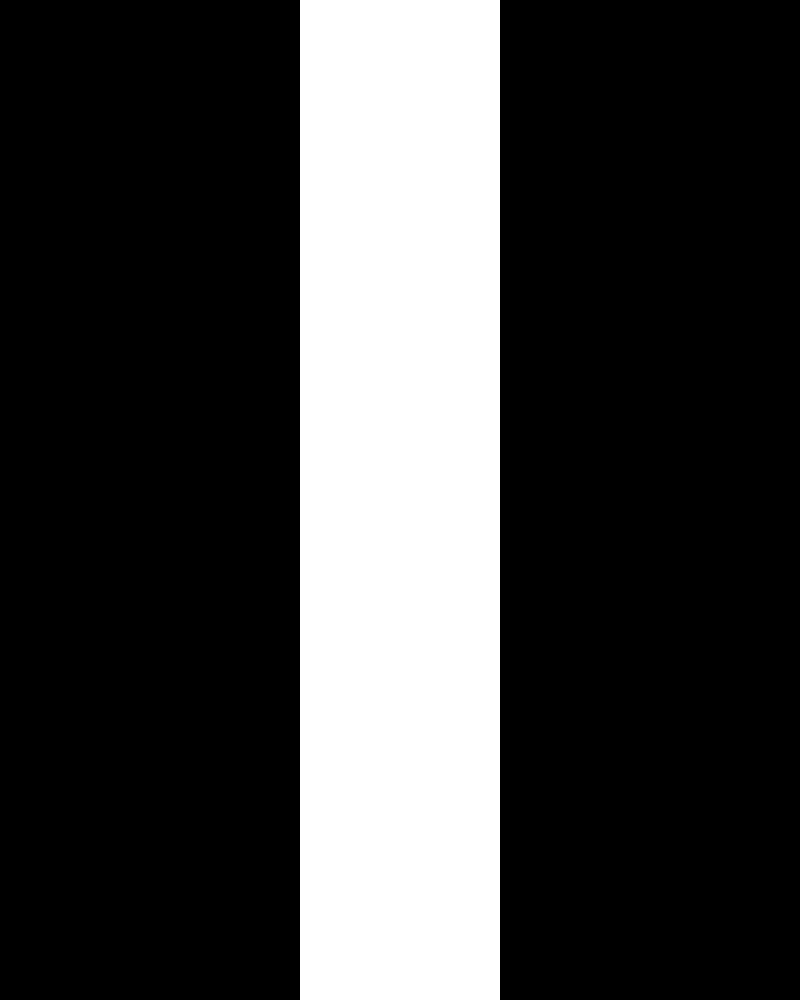
\includegraphics[height=.15\textheight]{corogfx/icon_pause.png} };}
  \only<5>{\tikz[transform shape,overlay] \node (quest) [darkred,below=of ar281,shift={(0ex,2.5ex)}] {???};}
  \end{onlyenv}

  \note{
  \begin{itemize}
  \item \alert<+>{how do we ensure the scheduler is there when we reach the first async io call? spawning lazy tasks; we initial suspend always; this ensures that when the body starts executing we already have the caller handle}
  \item \alert<+>{***TRANSITION*** now let's look at the functions}
  \item \alert<+>{***TRANSITION*** we start in outer}
  \item \alert<+>{***TRANSITION*** we suspend right away}
  \item ***TRANSITION*** we never reach body of middle, even though there is no reason to stop
  \end{itemize}
  }
\end{frame}

\begin{frame}[fragile]
  \frametitle{Symmetric transfer to the rescue}

  \begin{onlyenv}<1>
  \begin{lstlisting}[style=cpp20]
template<MyPromiseConcept OtherPromise_T>
void await_suspend((*@\danch(ar285)@*)std::coroutine_handle<OtherPromise_T> h(*@\danch(br285)@*)) {
  self.promise().my_caller = h;
  self.promise().my_scheduler = h.promise().my_scheduler;

}
  \end{lstlisting}
  \end{onlyenv}
  \begin{onlyenv}<2>
  \begin{lstlisting}[style=cpp20]
template<MyPromiseConcept OtherPromise_T>
(*@\danch(ar288)@*)auto(*@\danch(br288)@*) await_suspend((*@\danch(ar285)@*)std::coroutine_handle<OtherPromise_T> h(*@\danch(br285)@*)) {
  self.promise().my_caller = h;
  self.promise().my_scheduler = h.promise().my_scheduler;
  return (*@\danch(ar287)@*)self(*@\danch(br287)@*);
}
  \end{lstlisting}
  \monobox[orange](ar285:br285)
  \monobox[indigo](ar287:br287)
  \monobox[indigo](ar288:br288)
  \end{onlyenv}

  \note{
  This is co await in the caller.
  \begin{itemize}
  \item \alert<+>{closer look at suspend; what are the handles again?}
  \item ***TRANSITION*** self is handle to inner; we symmetric transfer to caller
  \end{itemize}
  }
\end{frame}

\begin{frame}[fragile]
  \frametitle{Symmetric transfer to the rescue}

  \begin{lstlisting}[style=cpp20]
Async<PartialResult> middle_function() {
(*@\danch(ar281)@*)  IoResult r = co_await inner_function();
  co_return PartialResult::from_io_result(r);
}
Async<Result> outer_function() {
(*@\danch(ar282)@*)  PartialResult r = co_await middle_function();
(*@\danch(ar283)@*)  co_return Result::from_partial_result(r);
}
  \end{lstlisting}

  \only<1-3>{\tikz[transform shape,overlay] \draw[>=triangle 45,->, darkred] ([shift={(-1em,0.25em)}]ar282.north) -- ([shift={(1em,0.25em)}]ar282.north);}
  \only<4>{\tikz[transform shape,overlay] \draw[>=triangle 45,->, darkred] ([shift={(-1em,0.25em)}]ar281.north) -- ([shift={(1em,0.25em)}]ar281.north);}
  %\only<3>{\tikz[transform shape,overlay] \node (pause) [darkred,above right=of ar283,shift={(65ex,6ex)}] { 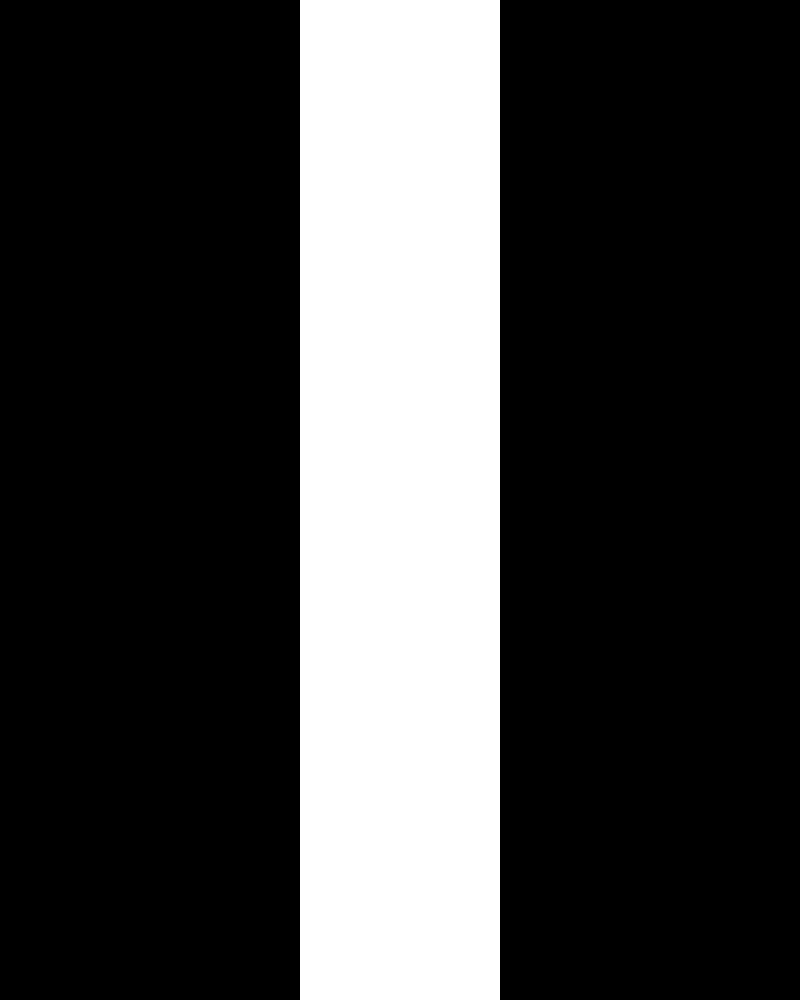
\includegraphics[height=.15\textheight]{corogfx/icon_pause.png} };}
  \only<4>{\tikz[transform shape,overlay] \node (pause) [darkred,above right=of ar283,shift={(65ex,-5ex)}] { 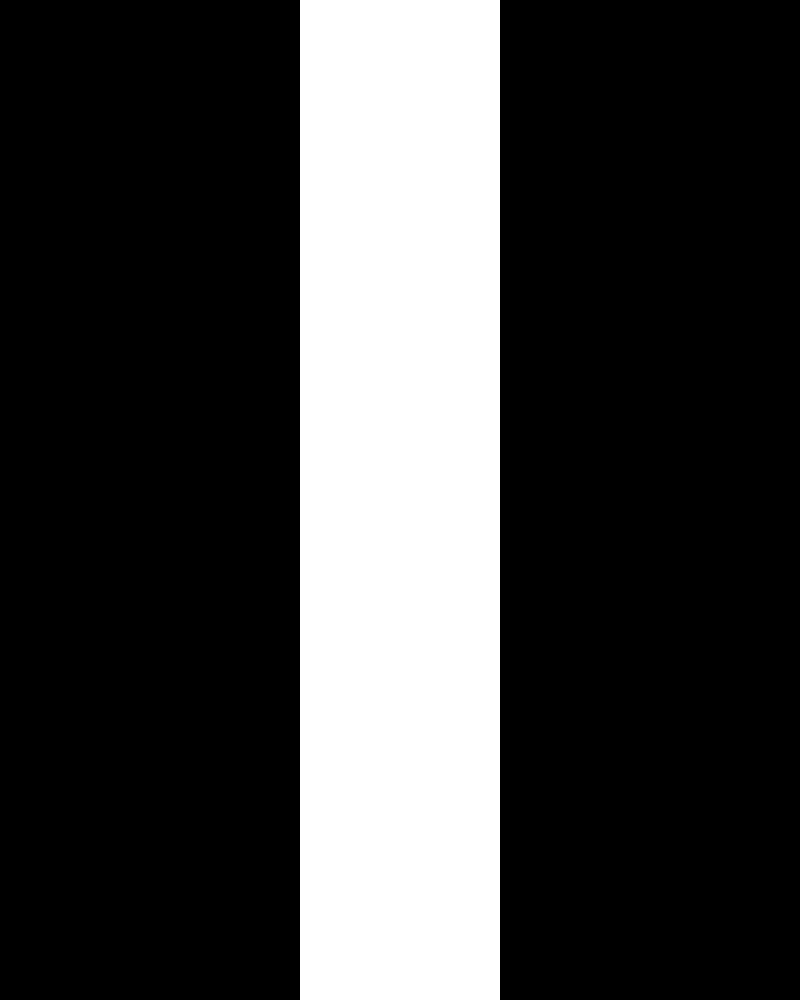
\includegraphics[height=.15\textheight]{corogfx/icon_pause.png} };}

  \begin{onlyenv}<1>
  \scalebox{0.75}{
  \begin{tikzpicture}[node distance=0mm and 5mm,overlay]
    \node (base) at ([shift={(17cm,6cm)}]0,0) [stackframe,fill=lightgray] {base()};
    \node (outer) [stackframe,above=of base,fill=orange!30]  {outer\_function()};
    \node (middle)   [stackframe,above=of outer,fill=indigo!30]              {middle\_function()};
    \node (getret)   [stackframe,above=of middle,fill=co_promise]            {initial\_suspend()};
  \end{tikzpicture}
  }
  \end{onlyenv}
  \begin{onlyenv}<2>
  \scalebox{0.75}{
  \begin{tikzpicture}[node distance=0mm and 5mm,overlay]
    \node (base) at ([shift={(17cm,6cm)}]0,0) [stackframe,fill=lightgray] {base()};
    \node (outer) [stackframe,above=of base,fill=orange!30]  {outer\_function()};
  \end{tikzpicture}
  }
  \end{onlyenv}
  \begin{onlyenv}<3>
  \scalebox{0.75}{
  \begin{tikzpicture}[node distance=0mm and 5mm,overlay]
    \node (base) at ([shift={(17cm,6cm)}]0,0) [stackframe,fill=lightgray] {base()};
    \node (outer) [stackframe,above=of base,fill=orange!30]  {outer\_function()};
    \node (middle)   [stackframe,above=of outer,fill=co_awaitable]              {await\_suspend};
  \end{tikzpicture}
  }
  \end{onlyenv}
  \begin{onlyenv}<4>
  \scalebox{0.75}{
  \begin{tikzpicture}[node distance=0mm and 5mm,overlay]
    \node (base) at ([shift={(17cm,6cm)}]0,0) [stackframe,fill=lightgray] {base()};
    \node (outer) [stackframe,above=of base,fill=indigo!30]  {middle\_function()};
  \end{tikzpicture}
  }
  \end{onlyenv}

  \note{
  \begin{itemize}
  \item \alert<+>{execute again, middle is on the stack, but we don't enter body because of initial\_suspend}
  \item \alert<+>{***TRANSITION*** back in outer we co\_await on the async returned by middle}
  \item \alert<+>{***TRANSITION*** await\_suspend initiates the symmetric transfer}
  \item ***TRANSITION*** now we enter body of middle; outer is suspended and no longer on stack!
  \end{itemize}
  }
\end{frame}

\begin{frame}
  \frametitle{Roadmap}
  \begin{todolist}
  \item \alert<3>{Spawn outermost coroutine and register scheduler}
  \only<1>{ \item \textcolor{darkred}{Call nested coroutines and propagate execution context} }
  \only<2>{ \item[\done] Call nested coroutines and propagate execution context}
  \item[\done] Suspend innermost coroutine
  \item[\done] Resume innermost coroutine
  \item[\done] Resume outer coroutine from inner coroutine
  \item Deliver final result
  \end{todolist}
\end{frame}

\begin{frame}
  \frametitle{Spawning a coroutine}
  % @todo
\end{frame}

\begin{frame}
  \frametitle{Roadmap}
  \begin{todolist}
  \only<1>{ \item \textcolor{darkred}{Spawn outermost coroutine and register scheduler} }
  \only<2>{ \item[\done] Spawn outermost coroutine and register scheduler}
  \item[\done] Call nested coroutines and propagate execution context
  \item[\done] Suspend innermost coroutine
  \item[\done] Resume innermost coroutine
  \item[\done] Resume outer coroutine from inner coroutine
  \item \alert<3>{Deliver final result}
  \end{todolist}
\end{frame}

\begin{frame}
  \frametitle{Joining a coroutine}
  % @todo
\end{frame}

\begin{frame}
  \frametitle{Roadmap}
  \begin{todolist}
  \item[\done] Spawn outermost coroutine and register scheduler
  \item[\done] Call nested coroutines and propagate execution context
  \item[\done] Suspend innermost coroutine
  \item[\done] Resume innermost coroutine
  \item[\done] Resume outer coroutine from inner coroutine
  \only<1>{ \item \textcolor{darkred}{Deliver final result}}
  \only<2>{ \item[\done] Deliver final result}
  \end{todolist}
\end{frame}


\begin{frame}[fragile]
  \frametitle{Taking it one step further...}
  
  \begin{onlyenv}<2>
  \begin{lstlisting}[style=cpp20]
struct (*@\danch(ar353)@*)promise_base(*@\danch(br353)@*) {
  promise_base* my_caller;
  promise_base* my_child;
};

template<typename T> struct Async { /* ... */
  struct promise_type : promise_base { /* ... */ };
};
  \end{lstlisting}
  \monobox[red](ar353:br353)
  \end{onlyenv}
  
  \begin{onlyenv}<3>
  \begin{lstlisting}[style=cpp20]
template<typename T>
concept MyPromise = std::derived_from<T, promise_base>;

template<typename T> struct (*@\danch(ar355)@*)Async(*@\danch(br355)@*) { /* ... */
  template<MyPromise (*@\danch(ar354)@*)OtherPromise_T(*@\danch(br354)@*)>
  auto await_suspend(std::coroutine_handle<OtherPromise_T> h) {
    // (*@\color{red}{\textit{establish a doubly-linked list}}@*)
    self.promise().my_caller = &(h.promise());
    h.promise().my_child = &(self.promise());
    return self;
  }
};
  \end{lstlisting}
  \monobox[red](ar354:br354)
  \monobox[green](ar355:br355)
  \end{onlyenv}
  
  \begin{onlyenv}<4>
  \begin{lstlisting}[style=cpp20]
struct (*@\danch(ar352)@*)promise_base(*@\danch(br352)@*) {
  promise_base* my_caller;
  promise_base* my_child;
  
  AnythingYouWant data;
};
  \end{lstlisting}
  \monobox[red](ar352:br352)
  \end{onlyenv}
  
  \note { \color{green}{TIME!} \color{black}{0:40} }
\end{frame}

\begin{frame}[fragile]
  \frametitle{Arbitrarily propagating data in the async call stack}
  
  \begin{lstlisting}[style=cpp20]
template<typename T>
struct (*@\danch(ar390)@*)Async(*@\danch(br390)@*) {
  void propagate(AnythingYouWant data);
};
  \end{lstlisting}
  \monobox[blue](ar390:br390)  \cpause
  
  \begin{lstlisting}[style=cpp20]
struct (*@\danch(ar391)@*)Propagate(*@\danch(br391)@*) {
  Propagate(AnythingYouWant data);
  // ...
};

Async<void> func() {
  // ...
  co_await Propagate(AnythingYouWant{ /* ... */ });
}
  \end{lstlisting}
  \monobox[green](ar391:br391)
  
\end{frame}


\begin{frame}[fragile]
  \frametitle{The call stack is now just another data structure}

  \begin{tikzpicture}[node distance = 0mm and 5mm,
    point/.style={circle,inner sep=0pt,minimum size=0pt,fill=black!100},
    memcell/.style={rectangle,minimum size=6mm,minimum width=26mm,thick,draw=black!80,font=\ttfamily},
   ]

    \node (rbp) {};

    \node (func1) [memcell,below=of rbp,style={minimum width=33mm}]  { Async<IoResult> };
    \filldraw[green, opacity=0.3][] (func1.south west)
        -- (func1.south east)
        -- (func1.north east)--cycle
        ;
    \filldraw[blue, opacity=0.3][] (func1.south west)
        -- (func1.north west)
        -- (func1.north east)--cycle
        ;
    \node (self1)   [memcell,below=of func1,style={minimum width=33mm}]  { self };
    \node (promise1)   [memcell,below=of self1,shift={(0ex,-5ex)}, fill={rgb,255:red,255; green,180; blue,180}]  { promise\_type };
    \node (caller1)   [memcell,below=of promise1]  { my\_caller };
    \node (callee1)   [memcell,below=of caller1,text=black!40]  { my\_child };

    \node (func2) [memcell,right=of func1,shift={(3ex,0)},style={minimum width=43mm}]  { Async<PartialResult> };
    \filldraw[green, opacity=0.3][] (func2.south west)
        -- (func2.south east)
        -- (func2.north east)--cycle
        ;
    \filldraw[blue, opacity=0.3][] (func2.south west)
        -- (func2.north west)
        -- (func2.north east)--cycle
        ;
    \node (self2)   [memcell,below=of func2,,style={minimum width=43mm}]  { self };
    \node (promise2)   [memcell,below=of self2,shift={(0ex,-5ex)}, fill={rgb,255:red,255; green,180; blue,180}]  { promise\_type };
    \node (caller2)   [memcell,below=of promise2]  { my\_caller };
    \node (callee2)   [memcell,below=of caller2]  { my\_child };

    \node (func3) [memcell,right=of func2,shift={(3ex,0)},style={minimum width=30mm}]  { Async<Result> };
    \filldraw[green, opacity=0.3][] (func3.south west)
        -- (func3.south east)
        -- (func3.north east)--cycle
        ;
    \filldraw[blue, opacity=0.3][] (func3.south west)
        -- (func3.north west)
        -- (func3.north east)--cycle
        ;
    \node (self3)   [memcell,below=of func3,style={minimum width=30mm}]  { self };
    \node (promise3)   [memcell,below=of self3,shift={(0ex,-5ex)}, fill={rgb,255:red,255; green,180; blue,180}]  { promise\_type };
    \node (caller3)   [memcell,below=of promise3]  { my\_caller };
    \node (callee3)   [memcell,below=of caller3]  { my\_child };

    \node (dotdot) [right=of caller3,shift={(4ex,0)}] {...};

    \draw[line width=0.5mm, black!80] (self1.south) edge[->] (promise1.north);
    \draw[line width=0.5mm, black!80] (self2.south) edge[->] (promise2.north);
    \draw[line width=0.5mm, black!80] (self3.south) edge[->] (promise3.north);
    \draw[line width=0.5mm, black!80] (caller1.east) edge[->] (promise2.west);
    \draw[line width=0.5mm, black!80] (caller2.east) edge[->] (promise3.west);
    \draw[line width=0.5mm, black!80] (caller3.east) edge[->] (dotdot.west);

    \draw[line width=0.5mm, black!80] (callee3.west) edge[->] (promise2.east);
    \draw[line width=0.5mm, black!80] (callee2.west) edge[->] (promise1.east);
  \end{tikzpicture}
\end{frame}

\iffalse % @todo
\begin{frame}[fragile]
  \frametitle{Terminating the \texttt{Async<>} chain}

  \begin{lstlisting}[style=cpp20]
(*@\danch(ar290)@*)Async<Result>(*@\danch(br290)@*) outer_function();

int main() {
  Async<Result> a = outer_function();
  invoke_async_function(a);
  Result r = a.get_result();
}
  \end{lstlisting}
  \mixedbox(ar290:br290)
\end{frame}

\begin{frame}[fragile]
  \frametitle{Terminating the \texttt{Async<>} chain}

  \begin{lstlisting}[style=cpp20]
template<typename T>
void invoke_async_function(Async<T>& f) {
  co_await f;
}

int main() {
  Async<Result> a = outer_function();
  invoke_async_function(a);
  Result r = a.get_result();
}
  \end{lstlisting}
\end{frame}
\fi

\begin{frame}
  \frametitle{Demo: Injecting scheduler and debugger inspection}
  
  \href{https://godbolt.org/z/d7EPTGTdd}{https://godbolt.org/z/d7EPTGTdd}
  
  \vspace{5pt}
  
  \only<1>{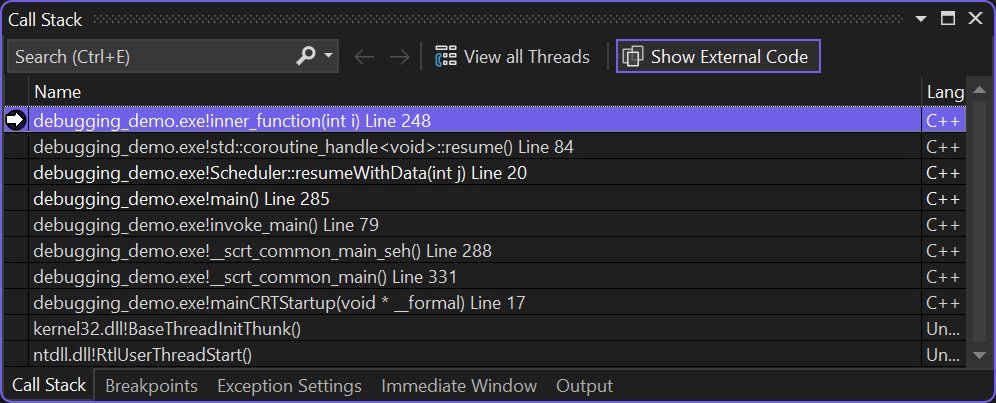
\includegraphics[width=\textwidth]{corogfx2/async_call_stack_0.png}}
  \only<2>{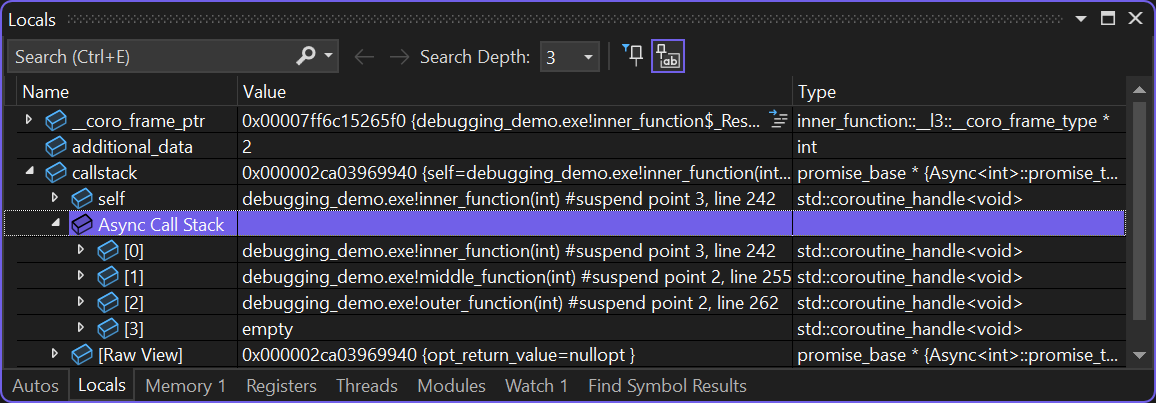
\includegraphics[width=\textwidth]{corogfx2/async_call_stack.png}}
  
\end{frame}


\begin{frame}
  \frametitle{The call stack is now just another data structure}
%  @todo more diagrams

  \begin{onlyenv}<1>
  \begin{center}
  \begin{tikzpicture}[node distance = 0mm and 5mm,
    memcell/.style={rectangle,minimum size=6mm,minimum width=60mm,thick,draw=black!80,font=\ttfamily},
   ]
    \node (promise2)   [memcell,shift={(0ex,-5ex)}, fill={rgb,255:red,255; green,180; blue,180}]  { promise\_type };
    \node (caller2)   [memcell,below=of promise2]  { my\_caller };
    \node (callee2)   [memcell,below=of caller2]  { my\_child };
  \end{tikzpicture}
  \end{center}
  \end{onlyenv}
  \begin{onlyenv}<2>
  \begin{center}
  \begin{tikzpicture}[node distance = 0mm and 5mm,
    memcell/.style={rectangle,minimum size=6mm,minimum width=60mm,thick,draw=black!80,font=\ttfamily},
   ]
    \node (promise2)   [memcell,shift={(0ex,-5ex)}, fill={rgb,255:red,255; green,180; blue,180}]  { promise\_type };
    \node (caller2)   [memcell,below=of promise2]  { my\_caller };
    \node (callee2)   [memcell,below=of caller2]  { std::vector<> my\_children };
  \end{tikzpicture}
  \end{center}
  \end{onlyenv}
  \begin{onlyenv}<3>
  \begin{center}
  \begin{tikzpicture}[node distance = 0mm and 5mm,
    memcell/.style={rectangle,minimum size=6mm,minimum width=60mm,thick,draw=black!80,font=\ttfamily},
   ]
    \node (promise2)   [memcell,shift={(0ex,-5ex)}, fill={rgb,255:red,255; green,180; blue,180}]  { promise\_type };
    \node (caller2)   [memcell,below=of promise2]  { std::vector<> my\_parents };
    \node (callee2)   [memcell,below=of caller2]  { std::vector<> my\_children };
  \end{tikzpicture}
  \end{center}
  \end{onlyenv}
  
  \note{
  \begin{itemize}
  \item Resume a function higher up the stack
  \item Splice two call stacks together
  \item Expose a range interface to use range algos over stack frames
  \item Still a structure of linearly nested tasks
  \item ***TRANSITION*** now it's a tree
  \item ***TRANSITION*** now it's a directed graph
  \end{itemize}
  }
\end{frame}

\iffalse
\begin{frame}
  \frametitle{C++ Coroutines - Evaluation}

  \begin{itemize}
  \item More efficient than threads
  \item Extremely flexible
  \item Introduces issues of function coloring\footnote{\href{https://journal.stuffwithstuff.com/2015/02/01/what-color-is-your-function/}{Bob Nystrom - What Color is Your Function? (2015)}}
  \item Building intuition is harder than with green threads, but maybe easier than callback-based async APIs
  \item Debugging experience benefits greatly from special tool support
  \end{itemize}

  \note{ \color{green}{TIME!} \color{black}{0:55} }
\end{frame}
\fi

\iffalse
\begin{frame}
  \frametitle{Conclusion}

  \begin{itemize}
  \item Coroutines allow for extremely powerful manipulation of control flow between functions
  \item To achieve best results, there should be some amount of uniformity between coroutine types
  \item C++26 senders/receivers are a first step in this direction, but a lot is still in development there
  \item C++ Coroutines are much more flexible than async/await in other languages. It is not yet clear what the best practices are for working with such a flexible feature.
  \item The community needs more people looking at this, trying interesting things, and joining the conversation
  \end{itemize}
\end{frame}
\fi

\iffalse

% Box drawing prototype code

\begin{frame}[fragile]
  \frametitle{Awaitable}

  \begin{lstlisting}[style=cpp20,numbers=left]
struct (*@\tikz[baseline,inner sep=0]\node[anchor=base](ar1001){};@*)Awaitable(*@\tikz[baseline,inner sep=0]\node[anchor=base](br1001){};@*) {
  bool await_ready();
  void await_suspend(std::coroutine_handle<(*@\tikz[baseline,inner sep=0]\node[anchor=base](cr1001){};@*)promise_type(*@\tikz[baseline,inner sep=0]\node[anchor=base](dr1001){};@*)>);
  void await_resume(); 
};
\end{lstlisting}

  \monobox[green](ar1001:br1001)
  \mixedbox(cr1001:dr1001)
\end{frame}


\begin{frame}[fragile]
  \frametitle{Awaitable}

  \begin{lstlisting}[style=cpp20,numbers=left]
struct (*@\danch(ar101)@*)Awaitable(*@\danch(br101)@*) {
  bool await_ready();
  void await_suspend(std::coroutine_handle<(*@\danch(cr101)@*)promise_type(*@\danch(dr101)@*)>);
  void await_resume(); 
};
\end{lstlisting}

  %\tikz[overlay]\filldraw[green, opacity=0.3] ([shift={(0,-0.5ex)}]ar101) rectangle ([shift={(0,2ex)}]br101);
  \tikz[overlay]\filldraw[green, opacity=0.3]
  ([shift={(0,2ex)}]br101.center)
    -- ([shift={(0,-0.5ex)}]ar101.center)
    -- ([shift={(0,-0.5ex)}]br101.center)
    -- cycle
    ;
  \tikz[overlay]\filldraw[blue, opacity=0.3]
  ([shift={(0,2ex)}]ar101.center)
    -- ([shift={(0,-0.5ex)}]ar101.center)
    -- ([shift={(0,2ex)}]br101.center)
    -- cycle
    ;

  %\tikz[overlay]\filldraw[red, opacity=0.3] ([shift={(0,-0.5ex)}]cr101) rectangle ([shift={(0,2ex)}]dr101);
  \mixedbox(cr101:dr101)
\end{frame}

\begin{frame}
  \frametitle{Awaitable}

  \begin{center}
    \tikz[baseline,inner sep=0]\node[anchor=base](ar2010){}; \tikz \draw node[pos=.5,scale=4,anchor=base]{Task}; \tikz[baseline,inner sep=0]\node[anchor=base](br2010){};
  \end{center}

  \tikz[overlay]\filldraw[green, opacity=0.3]
  ([shift={(0,12ex)}]br2010.center)
    -- ([shift={(0,0)}]ar2010.center)
    -- ([shift={(0,0)}]br2010.center)
    -- cycle
    ;
  \tikz[overlay]\filldraw[blue, opacity=0.3]
  ([shift={(0,12ex)}]ar2010.center)
    -- ([shift={(0,0)}]ar2010.center)
    -- ([shift={(0,12ex)}]br2010.center)
    -- cycle
    ;
\end{frame}
\fi

\begin{frame}
  \frametitle{Acknowledgements}
  Thanks to Lewis Baker and Mateusz Pusz for valuable feedback and discussions on this talk. Any remaining mistakes are my own.
  
  \note{ \color{green}{TIME!} \color{black}{0:45} }
\end{frame}


\begin{frame}
  \frametitle{Thanks for your attention.}

  \href{https://stackoverflow.com/users/577603/comicsansms}{
\includegraphics[height=.05\textheight]{resources/so-icon.png}}
  \href{https://github.com/ComicSansMS}{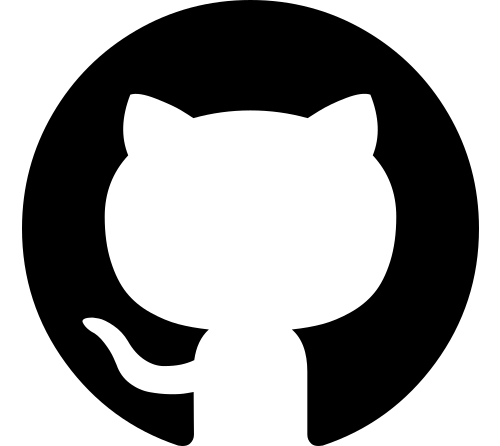
\includegraphics[height=.05\textheight]{resources/github-icon.png}}
  \includegraphics[height=.05\textheight]{resources/discord-icon.png} ComicSansMS /
  \href{mailto:cpp@andreas-weis.net}{
\includegraphics[height=.06\textheight]{resources/email-icon.png} cpp@andreas-weis.net}

\vspace{20pt}

\begin{center}
  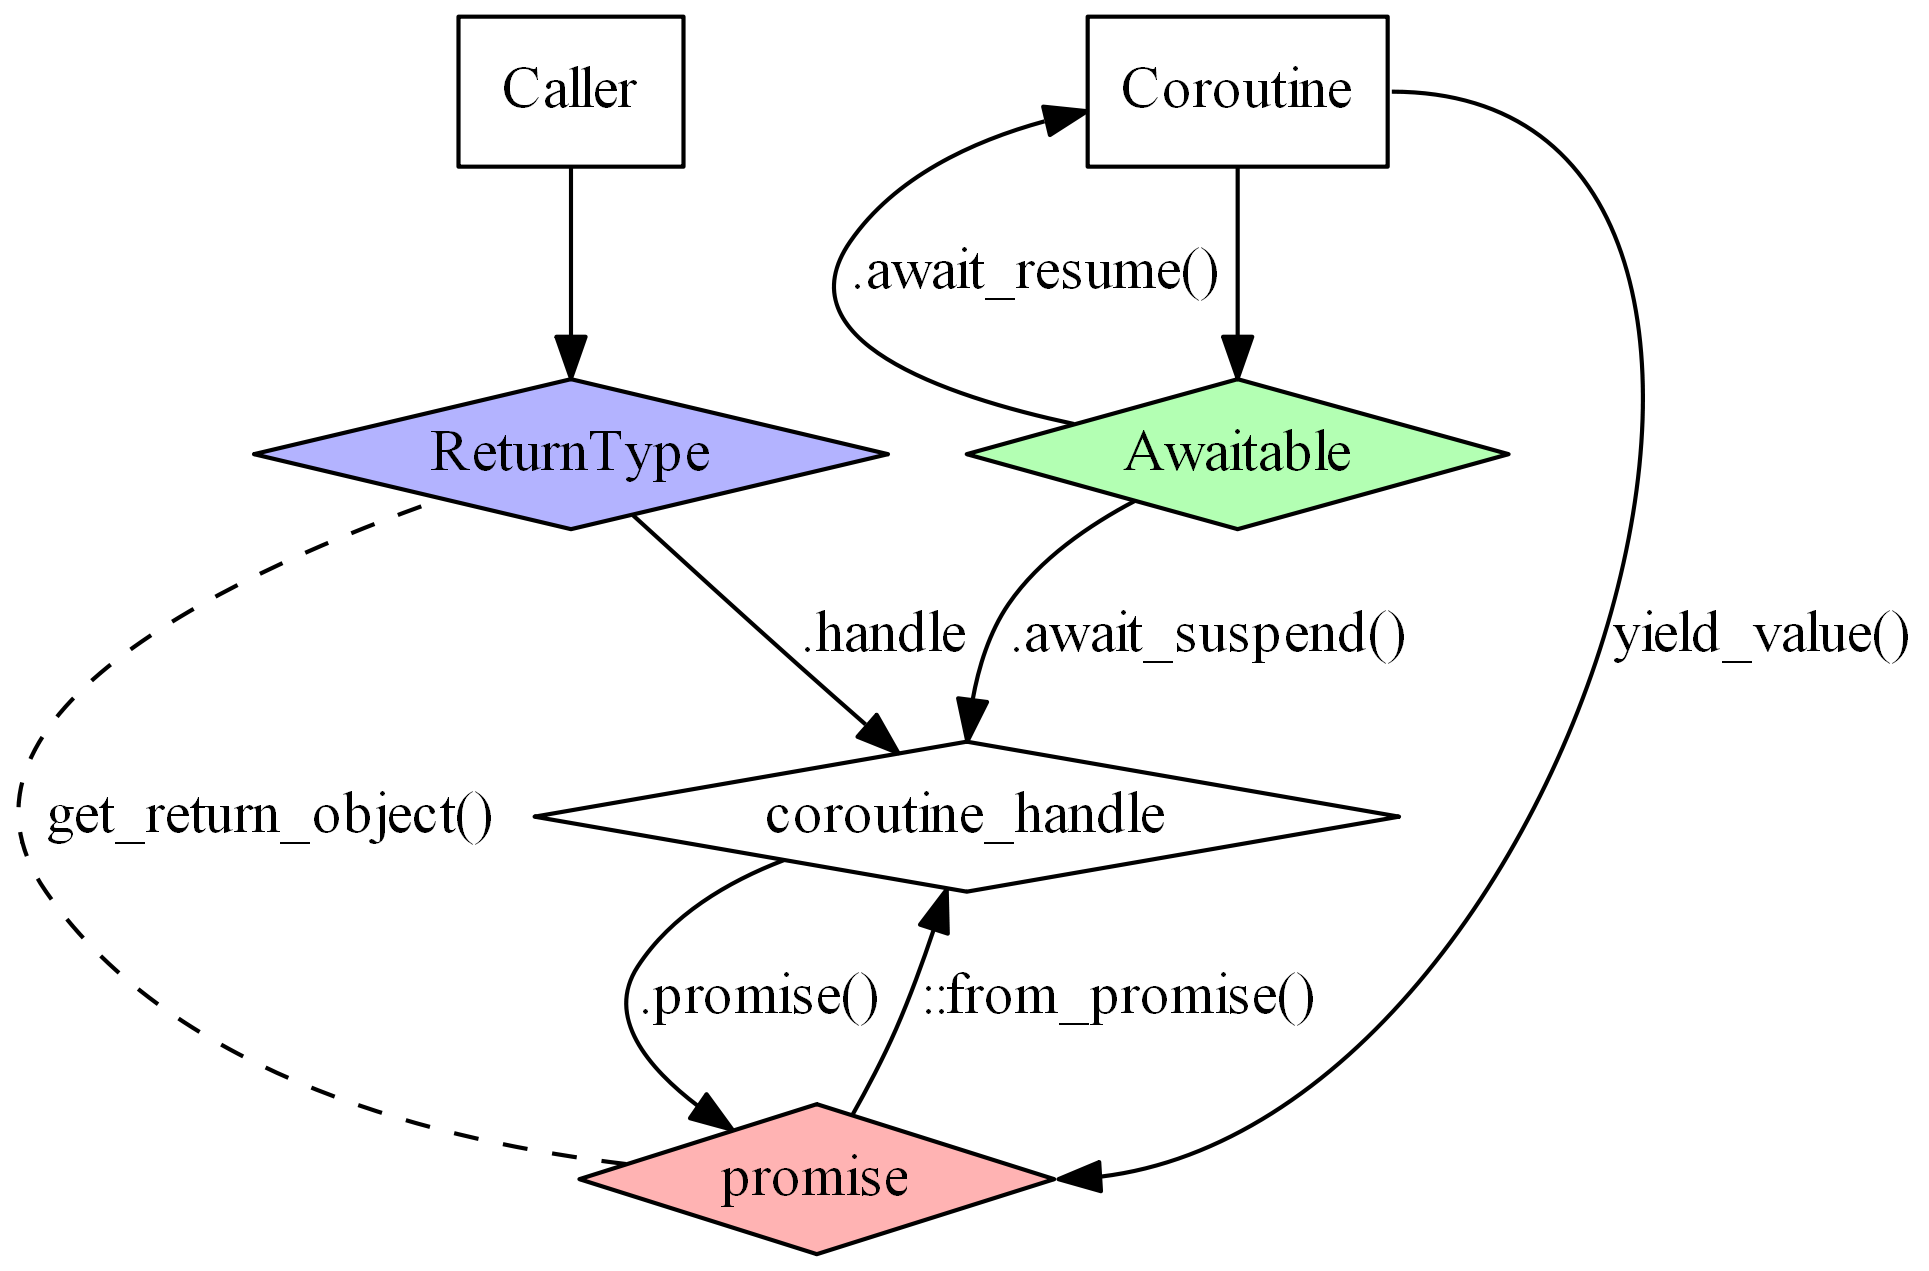
\includegraphics[height=.6\textheight]{corogfx/acquaintances05.png}
  \hspace{12ex}
  \href{https://github.com/ComicSansMS/cpp20_coroutine_cheat_sheet}{\includegraphics[height=.4\textheight]{corogfx/qrcode}}
\end{center}

\end{frame}


\end{document}
